\documentclass{article}
\usepackage{geometry}
\usepackage{amssymb}
\usepackage{amsthm}

\usepackage{ifdraft}
\usepackage{asymptote}
\usepackage{nccmath}
\usepackage{mathtools}

\allowdisplaybreaks

\usepackage{listings}

\lstset{
  basicstyle=\ttfamily,
  columns=fullflexible
}

\newcommand{\code}[1]{\lstinline!#1!}
\newcommand{\codebg}[2]{\setlength{\fboxsep}{0pt}\colorbox{#1}{\lstinline!#2!}}
\newcommand{\subno}[1]{\par\noindent\textbf{#1}}
\newcommand{\sT}{{\sf T}}

\ifoptiondraft
{
    \usepackage{showkeys}
    \geometry{paperheight=25cm,paperwidth=29cm,top=1.5cm,bottom=1.cm,left=7cm,right=7cm}
}
{
    \geometry{paperheight=25cm,paperwidth=17cm,top=1.5cm,bottom=1.cm,left=1cm,right=1cm}
}

\usepackage{algorithm}
\usepackage{algpseudocode}
\usepackage{float}

\usepackage{mlmodern}
\usepackage[T1]{fontenc}

\usepackage{dsfont}
\usepackage{bbm}

\usepackage{tikz}
\usetikzlibrary{matrix,fit,decorations.text,positioning,arrows.meta,patterns,shapes,math,calc}

\tikzset{mystyle/.style={draw,circle,label={[fill=yellow]0:#1}}}

\usepackage{fancyvrb}

\usepackage{physics}
\usepackage{tensor}
\usepackage{accents}

\usepackage[shortlabels]{enumitem}

\usepackage{titlesec}

\titleformat{\section}{\sffamily\Large\bfseries}{\thesection}{0.5em}{}
\titlespacing*{\section}
  {0pt}   % left indent
  {0.5ex} % space before title
  {0.5ex} % space after title  <-- reduce this
\titleformat{\subsection}[runin]
  {\sffamily\bfseries}   % bold+sans serif title
  {}                     % no number
  {0em}                  % space between number and title
  {}                     % code before title
  [.]                    % code after title
\titlespacing*{\subsection}
  {0pt}    % left
  {1.5ex}  % vertical space before heading
  {0.3em}  % horizontal space after heading  <-- reduce this

\usepackage{fancyhdr}
\fancypagestyle{main}{
    \fancyhf{}
    \addtolength{\topmargin}{-3.18243pt}
    \setlength{\headsep}{3pt}
    \fancyhead[R]{  
    \bfseries\footnotesize\thepage
    }  
}

\renewcommand{\footrulewidth}{0pt}% default is 0pt
\renewcommand{\headrulewidth}{0pt}% default is 0pt

\renewcommand{\headrulewidth}{0pt}
\setlength{\headheight}{23.5pt}

%This is for hypertext references
\usepackage{url}%this line and the next are related to hyperlinks
\usepackage[colorlinks=true, pdfstartview=FitV, linkcolor=blue, citecolor=blue, urlcolor=blue]{hyperref}

\usepackage{cleveref}
\usepackage{natbib}

\newcommand{\vd}{%
  \mathrel{%
    \tikz[baseline=(current bounding box.center)]{
    \fill[black] (0,0) circle [radius=.8pt];
    \fill[black] (0,.2) circle [radius=.8pt];
    \fill[black] (0,-.2) circle [radius=.8pt];
    }
  }%
}%

\newcommand{\rdd}{%
  \mathrel{%
    \tikz[baseline=(current bounding box.center)]{
    \fill[black] (0,0) circle [radius=.8pt];
    \fill[black] (-.2,.2) circle [radius=.8pt];
    \fill[black] (.2,-.2) circle [radius=.8pt];
    }
  }%
}%

\newcommand{\hd}{%
  \mathrel{%
    \tikz[baseline=(current bounding box.center)]{
    \fill[black] (0,0) circle [radius=.8pt];
    \fill[black] (-.2,0) circle [radius=.8pt];
    \fill[black] (.2,0) circle [radius=.8pt];
    }
  }%
}%

\newcommand{\hhd}{%
  \mathrel{%
    \tikz[baseline={([yshift=-.55ex]current bounding box.center)}]{
      \fill[black] (0,0) circle [radius=.8pt];
      \foreach \i in {1,2,...,5}{
      \fill[black] ({-.2*\i},0) circle [radius=.8pt];
      \fill[black] ({.2*\i},0) circle [radius=.8pt];
      }
    }
  }%
}%
\NewDocumentCommand{\drawhnodes}{ m m }   
{
    \tikzmath{
        coordinate \a, \b;
        int \i;
        \a = (#1.west);
        \b = (#1.east);
        \l = \bx - \ax;
        \dx = 5.0;
        \n = int(\l/\dx);
        \g = (\l - \n * \dx)/2.0 ;
        coordinate \c;
        for \i in {1,...,\n+1}{
            \c = ({\ax+\g+(\i-1)*\dx},\ay);
            {\filldraw[fill=#2,line width=0.1mm] (\c) circle (.2mm) ;};
        };
    }    
}

\NewDocumentCommand{\drawvnodes}{ m m }   
{
    \tikzmath{
        coordinate \a, \b;
        int \i;
        \a = (#1.north);
        \b = (#1.south);
        \l = \ay - \by;
        \dy = 5.0;
        \n = int(\l/\dy);
        \g = (\l - \n * \dy)/2.0 ;
        coordinate \c;
        for \i in {1,...,\n+1}{
            \c = (\ax,{\by+\g+(\i-1)*\dy});
            {\filldraw[fill=#2,line width=0.1mm] (\c) circle (.2mm) ;};
        };
    }
}

\newcommand{\Out}{\mathsf{O}}
\newcommand{\T}{\mathsf{T}}
\newcommand{\Q}{\mathsf{Q}}
\newcommand{\K}{\mathsf{K}}
\newcommand{\V}{\mathsf{V}}

\newcommand{\Z}{\mathbb{Z}}
\newcommand{\R}{\mathbb{R}}
\newcommand{\cR}{\mathcal{R}}

\newcommand{\vc}{\symbf{c}}
\newcommand{\vw}{\symbf{w}}

\NewDocumentCommand{\ubar}{m}{%
  \underaccent{\bar}{#1}%
}

\DeclareMathOperator{\softmax}{softmax}
\DeclareMathOperator{\g}{g}
\DeclareMathOperator*{\argmin}{argmin}
\DeclareMathOperator{\diag}{diag}
\DeclareMathOperator{\im}{im}
\DeclareMathOperator{\id}{id}
\DeclareMathOperator{\sspan}{span}

\newtheoremstyle{pprop}
                {\topsep} % space above
                {\topsep} % space below
                {\normalshape} % body font
                {0pt} % indent amount
                {\bfseries} % head font
                {} % punctuation after head
                {0pt} % space after theorem head
                {\thmname{#1}\thmnumber{ #2}\thmnote{ (#3)}\\[6pt]} % theorem head spec
                
\theoremstyle{pprop}
\newtheorem{problem}{Problem}[section]
\setcounter{section}{2}
\begin{document}
\pagestyle{main}
\begin{center}
    \sffamily\LARGE\bfseries Linear Algebra and Optimization 
\end{center}
The answers here are for the problems in \citep{gallier2020linear}. 
They reflect my effort to answer them and in no way should be 
construed as the approved solutions for this book. 
\section*{Chapter 2}
\begin{problem}
\noindent\textbf{1.} To prove that $(H,\cdot)$ is a group we must show that the following properties hold:
\begin{enumerate}[(1)]
  \item \textbf{Closure}:  if $A,B \in {H}$ then $A \cdot B \in {H}$. To show this note that any upper triangular 
  matrix $A$ has the property
  \[
  \begin{bmatrix}
1 & a & b \\
0 & 1 & c \\
0 & 0 & 1
\end{bmatrix}
=
\begin{bmatrix}
1 & a & b \\
d & 1 & c \\
e & f & 1
\end{bmatrix}
\odot
\begin{bmatrix}
1 & 1 & 1 \\
0 & 1 & 1 \\
0 & 0 & 1
\end{bmatrix}
  \]
  where $\odot$ denotes the \textbf{Hadamard} product of two matrices and the first matrix is non-singular. In index notation we write this as 
  \[
  A_{ij} = a_{ij} \mathbbm{1}_{j \geq i}
  \]
  where $\mathbbm{1}_{\text{statement}}=1$ if the statement is true and zero otherwise. Then
\begin{align*}
(A \cdot B)_{ij}&=\sum_{k=1}^n A_{ik}B_{kj}=\sum_{k=1}^n a_{ik}b_{kj}
\mathbbm{1}_{k \geq i}\mathbbm{1}_{j \geq k} \\
& =\sum_{k=1}^n a_{ik}b_{kj}\mathbbm{1}_{j \geq i}
=(a \cdot b)_{ij}\mathbbm{1}_{j \geq i}
\end{align*}
and so, $A \cdot B \in {H}$.
\item Since $H$ is a subspace of the vector space of $3 \times 3$ matrices it inherits associativity and the identity element.
\item The inverse $A^{-1}$ of $A \in  H$ must have the property 
\[
A \cdot A^{-1} = A^{-1} \cdot A = I, \quad A^{-1} \in  H.
\]
We note that, since we can write any uppper-triangular matrix as the Hadamard product of a standard matrix and an upper-triangular 
matrix of ones, then 
\[
(A \cdot A^{-1})_{ij}=\sum_{k=1}^n a_{ik}a^{-1}_{kj}
\mathbbm{1}_{k \geq i} \mathbbm{1}_{j \geq k} = 
\sum_{k=1}^n \delta_{ij}\mathbbm{1}_{k \geq i} \mathbbm{1}_{j \geq k}
=\delta_{ij}
\]
where $\delta_{ij}=1$ if $i=j$ and zero otherwise. Therefore the inverse exists and is an element of $H$. The following explicit form 
of the inverse
\[
\begin{bmatrix}
1 & a' & b' \\
0 & 1 & c' \\
0 & 0 & 1
\end{bmatrix}
\] 
satisfies the diagonal and lower triangular conditions. For the upper triangular elements we must have  
\begin{align*}
a'+a & = 0 \\
b'+ac'+b & = 0 \\
c'+c & = 0
\end{align*}
and so 
\[
A^{-1}=\left[\begin{matrix}1 & - a & a c - b\\0 & 1 & - c\\0 & 0 & 1\end{matrix}\right].
\]
If $({ H},\cdot)$ is abelian then $A \cdot B = B \cdot A$ or 
\begin{align*}
(A\cdot B)_{ij} & =
\sum_{k=1}^n a_{ik} b_{kj} \mathbbm{1}_{k \geq i} \mathbbm{1}_{j \geq k} =
\mathbbm{1}_{j \geq i}\sum_{k=1}^n a_{ik} b_{kj} = \mathbbm{1}_{j \geq i}
(a \cdot b)_{ij},\\
(B \cdot A)_{ij} & = \sum_{k=1}^n b_{ik} a_{kj}  \mathbbm{1}_{k \geq i} \mathbbm{1}_{j \geq k} = 
\mathbbm{1}_{j \geq i}\sum_{k=1}^n b_{ik} a_{kj} 
=\mathbbm{1}_{j \geq i} (b \cdot a).
\end{align*}
Since $a \cdot b \neq b \cdot a$ we conclude that $H$ is not abelian.
\end{enumerate}
\noindent\textbf{2.} If $a \in G_1$ then from the definition of $e_1$
\[
\phi(a e_1 )=\phi(a) \in G_2
\]
and since $\phi$ is a homomorphism 
\[
\phi(a e_1)=\phi(a) \phi(e_1).
\]
Hence
\[
\phi(a) \phi(e_1)=\phi(a)
\]
and we conclude that $\phi(e_1)=e_2$.

Since $a a^{-1} = e_1$
$$
\phi(a a^{-1})=\phi(a) \phi(a^{-1})=\phi(e_1).
$$
We have already shown that $\phi(e_1)=e_2$. Therefore  $\phi(a^{-1})=\phi(a)^{-1}$.
\par\noindent\textbf{3.} For any $A \in H$, elements $a, b , c \in \mathbb{R}$. Since if $b \in \mathbb{R}$, $e^{ib}$ 
generates all elements of $S^1$ we conclude that $\phi$ is surjective.

To prove that $(G,\cdot)$ first note that closure is a consequence of the closure of $\mathbb{R}$ w.r.t. addition and multiplication 
and the fact that if $u_1,u_2 \in S^1$ then, since $e^{ix_1y_2} \in S_1$, $e^{ix_1y_2}u_1 u_2 \in S_1$ (closure of $S^1$ under 
multiplication). To prove associativity write
\begin{align*}
& ((x_1,y_1,u_1)\cdot(x_2,y_2,u_2))\cdot(x_3,y_3,u_3)=\\
& \kern3ex=   (x_1+x_2,y_1+y_2,e^{ix_1y_2}u_1u_2)\cdot(x_3,y_3,u_3)=\\
& \kern3ex= (x_1+x_2+x_3,y_1+y_2+y_3,e^{i(x_1+x_2)y_3}e^{ix_1y_2}u_1u_2u_3)=\\
& \kern3ex=
(x_1+(x_2+x_3),y_1+(y_2+y_3),e^{ix_1(y_2+y_3)}u_1(e^{ix_2y_3}u_2u_3))=\\
& \kern3ex=
(x_1,y_1,u_1)\cdot(x_2+x_3,y_2+y_3,e^{ix_2y_3}u_2u_3)=\\
& \kern3ex=
(x_1,y_1,u_1)\cdot((x_2,y_2,u_2)\cdot(x_3,y_3,u_3)).
\end{align*}
The identity element of $G$, $(0,0,1)$ borrows the identity elements of$(\mathbb{R},+)$ and $(S^1,\cdot)$. 
The inverse of $(x,y,u)$ must have the property 
$$
(x,y,u)\cdot(x',y',u')=(x+x',y+y',e^{ixy'}uu')=(0,0,1)
$$
and so $x'=-x,\ y'=-y, \ u'=e^{ixy}u^{-1}$. $\phi$ is a homomorphism if for $A,B \in H$
$$
\phi(A \cdot B) = \phi(A) \cdot \phi(B).
$$
Since
$$
\begin{bmatrix}
1 & a & b \\
0 & 1 & c \\
0 & 0 & 1
\end{bmatrix}
\begin{bmatrix}
1 & d & e \\
0 & 1 & f \\
0 & 0 & 1
\end{bmatrix}=
\begin{bmatrix}
1& a+ d & af +b + e \\
0 & 1 & c+ f \\
0 & 0 & 1
\end{bmatrix},
$$
we have
\begin{align*}
\phi(A \cdot B) & =(a+d, c+f,e^{i(af+b+e)}) \\
& =(a,c,e^{ib}) \cdot (d,f,e^{ie}) \\
& = \phi(A) \cdot \phi(B).
\end{align*}
\par\noindent\textbf{4.} We are looking for a set of matrices $A \in  H$ such that 
$$
\phi(A)=(0,0,1)
$$
the identity element in $G$. From the definition of $\phi$ we must have
$$
a=0, c=0, b =2\pi n
$$
where $n \in \mathbb{Z}$. For any $A \in \ker\phi$ we can write $A=I + 2\pi n E_{13}$. Closure follows since if $A,B\in\ker\phi$ 
\begin{align*}
A \cdot B & = (I + 2 \pi E_{13})\cdot(I + 2\pi m E_{13})\\
& = I +2 \pi (n+m) E_{13} + (2\pi)^2nm E_{13}^2\\  
& =I +2 \pi (n+m) E_{13}  \in \ker\phi.
\end{align*}
Associativity is inherited; the identity element is $I$ ($n=0$) while the inverse of $A=I + 2\pi n E_{13}$ is 
$A^{-1}=I - 2\pi n E_{13}$. Hence $\ker\phi$ is a subgroup of $ H$.
\end{problem}
\begin{problem}
  To check that $m\mathbb{Z}=\{mk \vert k\in \mathbb{Z}\}$ is an abelian subgroup of $\mathbb{Z}$ first note that 
  $mk_1+mk_2=m(k_1+k_2)$ (closure). Addition is commutative/associative in $\mathbb{Z}$ and $m\mathbb{Z}$ inherits these 
  properties. It also inherits the identity element ($k=0$) and the inverse ($k^{-1}=-k$).
  \par\noindent\textbf{1.} $\phi(mk):=k$; this is an homomorphism since 
$$
\phi(mk_1+mk_2)=\phi(m(k_1+k_2))=k_1+k_2=\phi(mk_1)+\phi(mk_2).
$$
Since $\ker\phi=\{0\}$ it is also an isomorphism.
\par\noindent\textbf{2.} If $i(mk):=mk$ then
$$
i(mk_1+mk_2)=i(m(k_1+k_2))=m(k_1+k_2)=\\mk_1+mk_2=
i(mk_1)+i(mk_2)
$$
hence the inclusion map is a group homomorphism. If $p:\mathbb{Z} \to m\mathbb{Z}$ is a homomorphism then
$$
p (l_1+l_2)=p(l_1)+p(l_2)=mk_1+m k_2
$$
where $l_1,l_2,k_1,k_2 \in \mathbb{Z}$ (for example $k=\lfloor l/m  \rfloor$). If $p \circ i={\rm id}$ then $p$ is the 
left inverse of $i$. By Proposition 2.16, $i$ must be an isomorphism. However, unless $m=1$, $i$ is not an isomorphism since 
it is not surjective.
\end{problem}
\begin{problem}
  As defined $E$ is an abelian group w.r.t. $+$.
From the definition of $\cdot$ we have 
\begin{align*}
\lambda\cdot((x_1,y_1)+(x_2,y_2)) & =\lambda\cdot(x_1+x_2,y_1+y_2) 
=(\lambda(x_1+x_2),y_1+y_2)=(\lambda x_1+\lambda x_2,y_1+y_2)\\
& =(\lambda x_1,y_1)+(\lambda x_2,y_2)=\lambda\cdot(x_1,y_1)+\lambda\cdot(x_2,y_2)
\end{align*}
so axiom $\text{(V1)}$ holds. 
\begin{align*}
(\lambda + \mu) \cdot (x,y) & =((\lambda+\mu)x,y)=(\lambda x + \mu x,y) =(\lambda x,y)+(\mu x,0) \\
& =\lambda\cdot(x,y)+\mu\cdot(x,0)\neq\lambda\cdot(x,y)+\mu\cdot(x,y)
\end{align*}
so axiom $\text{(V2)}$ fails.
$$
(\lambda \mu)\cdot(x,y)=((\lambda\mu)x,y)=(\lambda(\mu x),y)\\=\lambda\cdot(\mu x,y)=\lambda\cdot(\mu\cdot(x,y))
$$
so axiom $\text{(V3)}$ holds.
$$
1\cdot(x,y)=(1*x,y)=(x,y)
$$
so axiom $\text{(V4)}$ holds.
\end{problem}
\begin{problem}
\noindent\textbf{1.} Below we (mostly) omit steps that use the properties of a field. 
\begin{align*}
\alpha\cdot 0&=\alpha\cdot(u-u), & \text{\footnotesize any vector $u$ has an additive inverse} \\
&=\alpha \cdot u - \alpha \cdot u, & \text{\footnotesize (V1)} \\
& =0, & \text{\footnotesize the additive inverse of $\alpha \cdot u$ is $-\alpha \cdot u$}
\end{align*}   
\begin{align*}
0 \cdot v &= (\alpha - \alpha) \cdot v, & \text{\footnotesize$K$ is a field} \\
& = \alpha \cdot v - \alpha \cdot v, & \text{\footnotesize (V2)} \\
& =0, & \text{\footnotesize the additive inverse of $\alpha \cdot v$ is $-\alpha \cdot v$}
\end{align*}
\begin{align*}
\alpha \cdot (-v) & = \alpha \cdot (-1 \cdot v) & \\
& = (\alpha * -1) \cdot v, & \text{\footnotesize (V3)} \\
& = - (\alpha \cdot v)  & 
\end{align*}
\begin{align*}
(-\alpha) \cdot v & = (-1 *\alpha) \cdot v & \\
& = -1\cdot (\alpha\cdot v), & \text{\footnotesize (V3)} \\
& = - (\alpha \cdot v), & \text{\footnotesize the additive inverse of $\alpha \cdot v$ is $-1\cdot(\alpha \cdot v)$} 
\end{align*}
\par\noindent\textbf{2.} Axiom $\text{(V2)}$ states that 
$$
\alpha\cdot(u+v)=\alpha\cdot u + \alpha \cdot v
$$
where $u,v$ are vectors and $\alpha$ is a scalar. Then 
\begin{align*}
\alpha \cdot x &= \alpha \cdot (x_1 e_1 + x_2 e_2 + \cdots + x_n e_n) \\
& = \alpha \cdot (x_1 e_1 + ( x_2 e_2 + \cdots + x_n e_n)) \\
& = \alpha \cdot (x_1 e_1)+ \alpha \cdot (x_2 e_2 + \cdots + x_n e_n) \\
& \kern15ex \vdots \\
& = \alpha \cdot (x_1 e_1)+\cdots + \alpha \cdot (x_{n-2} e_{n-2})+
\alpha \cdot(x_{n-1}e_{n-1}+ x_n e_n) \\
& = \alpha\cdot (x_1 e_1)+ \cdots + \alpha\cdot(x_n e_n).
\end{align*}
Since for any $i=1,2,\ldots,n$, 
$$
\alpha\cdot(x_i e_i)=\alpha\cdot(x_i\cdot e_i)=(\alpha * x_i) \cdot e_i \\
=(x_i * \alpha) \cdot e_i=x_i\cdot(\alpha\cdot e_i)
$$
given $\{\alpha \cdot e_i\}_{i=1}^n$ we can determine the result of scalar multiplication on any vector by its 
action on the basis vectors.
\par\noindent\textbf{3.} Lets work backwards. We want to define scalar multiplication so that 
$$1 \cdot u \neq u;$$
if we denote $1\cdot u=\nu(u)$ then if axiom $\text{(V3)}$ holds 
$$
(1*1)\cdot u=1\cdot(1 \cdot u)=1\cdot \nu(u)=\nu^2(u).
$$
Since $1*1=1$ we conclude that $\nu(u)=\nu^2(u)$ and so, in this setting, scalar multiplication must be a projection. One example is 
$$
\alpha \cdot x=(\alpha x_1,\ldots,\alpha x_{n-1},0)
$$
which for $\alpha=1$ gives the desired result. All other axioms follow; for example
\begin{align*}
\alpha\cdot(x+y)&=(\alpha(x_1+y_1),\ldots,\alpha(x_{n-1}+y_{n-1}),0) \\
& =(\alpha x_1 ,\alpha x_{n-1},0)+(\alpha y_1,\ldots,\alpha y_{n-1},0) \\
& = \alpha \cdot x + \alpha \cdot y.
\end{align*}
\par\noindent\textbf{4.} If $n \in \mathbb{N}$ then according to $\text{(V2)}$
\begin{align*}
n\cdot x & = (1+ \cdots + 1) \cdot x \\
& = 1 \cdot x + \cdots + 1 \cdot x \\ 
& = (y_1,\ldots,y_n)+ \cdots+(y_1,\ldots,y_n)\\
& = (n y_1,\ldots, n y_n)=n(y_1,\ldots,y_n)\\
&= n(1 \cdot x).
\end{align*}
Next use $\text{(V3)}$:
$$
1\cdot x =\left( \frac{1}{n}* n\right)\cdot x=n\cdot\left(\frac{1}{n} \cdot x\right)=(1+\cdots+1)\cdot \left(\frac{1}{n}\cdot x\right). 
$$
If $\frac{1}{n}\cdot x=(y_1',\ldots,y_n')$ then since $1\cdot x=(y_1,\ldots,y_n)$ we must have
$$
(y_1,\ldots,y_n)=(ny_1',\ldots,n y_n').
$$
This is possible only if $y_i'=y_i/n$ for $i=1,\ldots,n$ and so we find that
$$
\frac{1}{n}\cdot x=\frac{1}{n}(1 \cdot x).
$$

A rational number $r=m/n$ where $m,n \in \mathbb{N}$; then
\begin{align*}
\frac{m}{n}\cdot x & = \left( m * \frac{1}{n} \right) \cdot x =m \cdot \left(  \frac{1}{n} \cdot x\right)=m \cdot \left(\frac{1}{n} (1\cdot x)  \right) \\
& =\frac{1}{n}\left(m \cdot (1 \cdot x)\right)=\frac{1}{n}\left(1 \cdot (m \cdot x)\right)=\frac{1}{n}\left( 1 \cdot m (1\cdot x) \right)\\
& =\frac{m}{n}(1\cdot(1\cdot x))=r((1*1)\cdot x)=r(1 \cdot x).
\end{align*}
Any vector $x$ has the following expansion given a basis $\{e_1,\ldots,e_n\}$:
$$
x= x_1 e_1 + \cdots + x_n e_n.
$$
Given $1\cdot x =y$ and 
$$
y=y_1 e_1 + \cdots + y_n e_n
$$
we have 
$$
1\cdot x = x_1 (1\cdot e_1)+\cdots+x_n (1\cdot e_n).
$$
Define $1 \cdot e_i = \sum_{j=1}^n \nu_{ji} e_j$ where $\nu_{ji}$ are scalars. Then 
$$
y_i = \sum_{j=1}^n \nu_{ji}x_i.
$$
So, given any vector $x$, and the coefficients $\nu$ that determine the action of 1 on a basis of $\mathbb{R}^n$ we 
can determine $1 \cdot x$.  Then since $r \cdot x=r y$ we can determine the action of any scalar multiplication.
\end{problem}
\begin{problem}
Linear independence requires that 
$$
a\begin{pmatrix}2\\1\\-3 \end{pmatrix}
+
b\begin{pmatrix}3\\2\\-5 \end{pmatrix}
+
c\begin{pmatrix}1\\-1\\1 \end{pmatrix}=0
\Rightarrow a=b=c=0.
$$
Starting from 
\begin{align*}
2a+3b+c & = 0 \\
-3a-5b+c &=0
\end{align*}
we obtain
$$
5a-8b=0.
$$
Then from
\begin{align*}
2a+3b+c & = 0 \\
a+2b-c &=0
\end{align*}
we have
$$
3a+5b=0.
$$
The only solution to this system of equations is $a=b=0$ since
$$
3(5a-8b)-5(3a+5b)=-b=0
$$
and then $5a=0$. Substitute $a=b=0$ in any of the three equations to obtain $c=0$.
The basis expansion of $x=(6,2,-7)$ in terms of these three independent vectors requires that
$$
a\begin{pmatrix}2\\1\\-3 \end{pmatrix}
+
b\begin{pmatrix}3\\2\\-5 \end{pmatrix}
+
c\begin{pmatrix}1\\-1\\1 \end{pmatrix}=
\begin{pmatrix}6\\2\\-7 \end{pmatrix}.
$$
It is easy to show that $a=b=c=1$.
\end{problem}
\begin{problem}
We want to show that
$$
\begin{pmatrix}
1 \\ 3 \\ -1 \\ 0
\end{pmatrix}=
a
\begin{pmatrix}
1 \\ 2 \\ -1 \\ -2
\end{pmatrix}
+b
\begin{pmatrix}
2 \\ 3 \\ 0 \\ -1
\end{pmatrix}
+c
\begin{pmatrix}
1 \\ 2 \\ 1 \\ 3
\end{pmatrix}
$$ 
for at least one of $a,b,c$ different from zero. Since we must have   
$$
-a+c=-1, \quad -2a-b+3c=0
$$
we can write $a=1+c$,  $b=c-2$. We are now left with 
\begin{align*}
a+2b+c&=1, \quad c+1+2(c-2)+c=1, \quad 4c=4 \\
2a+3b+2c&=3, \quad 2(c+1)+3(c-2)+2c=3, \quad 7c=7
\end{align*}
both of which have solution $c=1$. Then $a=2,\ b=-1$.

It is easy to show that the first three columns are independent. Hence the columns of $A$ span a subspace of $\mathbb{R}^4$. 
Therefore it is possible that the vector given cannot be expressed as a linear combination of the columns of $A$. 
After some rather tedious calculations that's what we find.
\end{problem}
\begin{problem}
Linear independence requires that 
$$
a\begin{pmatrix} 1 \\ 1 \\ 1\end{pmatrix}
+
b\begin{pmatrix} 1 \\ 1 \\ 2\end{pmatrix}
+
c\begin{pmatrix} 1 \\ 2 \\ 3\end{pmatrix}=0 \Rightarrow a=b=c=0.
$$  
From the first equation we have $c=-(a+b)$; then, for the other two equations,
\begin{align*}
a&=2b ,\qquad a=3b
\end{align*}
which only has a solution if $a=b=0$. It follows that $c=0$. Next 
$$
x_1\begin{pmatrix} 1 \\ 1 \\ 1\end{pmatrix}
+x_2\begin{pmatrix} 1 \\ 1 \\ 2\end{pmatrix}
+x_3\begin{pmatrix} 1 \\ 2 \\ 3\end{pmatrix}=\begin{pmatrix} 6 \\ 9 \\ 14\end{pmatrix}
$$
is solved for $x_1=1,x_2=2,x_3=3$.
\end{problem}
\begin{problem}
Linear independence requires  
$$
a\begin{pmatrix}1 \\ 2 \\-1\\-2\end{pmatrix}
+
b\begin{pmatrix}2 \\ 3 \\0\\-1\end{pmatrix}
+
c\begin{pmatrix}1 \\ 2 \\1\\4\end{pmatrix}
+d\begin{pmatrix}1 \\ 3 \\-1\\0\end{pmatrix}=0
\Rightarrow a=b=c=d=0.
$$  
Use
\begin{align*}
2(a+2b+c+d)-(2a+3b+2c+3d)=0\Rightarrow b=d
\end{align*}
to rewrite the condition as
$$
a\begin{pmatrix}1 \\ 2 \\-1\\-2\end{pmatrix}
+
b\begin{pmatrix}3 \\ 6 \\-1\\-1\end{pmatrix}
+
c\begin{pmatrix}1 \\ 2 \\1\\4\end{pmatrix}
=0
$$
Next
$$
(a+3b+c)+(-a-b+c)=0\Rightarrow b=-c
$$
and 
$$
a\begin{pmatrix}1 \\ 2 \\-1\\-2\end{pmatrix}
+
b\begin{pmatrix}2 \\ 4 \\-2\\-5\end{pmatrix}
=0
$$
It is clear that $(1,2,-1,-2)$ and $(2,4,-2,-5)$ are independent.
Hence $a=b=0$ and, from the last two equations $c=d=0$.

The coordinates of $x$ are $(0,2,1,2)$
\end{problem}
\begin{problem}
The hint given uses the fact that if two vectors are orthogonal then they are independent. Since the rows of $H^{\sf T}$ contain the 
columns of $H$, independence requires that $H^{\sf T}H$ is a diagonal matrix:  
$$
\begin{bmatrix}
1 & 1 & 1 & 1 \\
1 & 1 & -1 & -1 \\
1 & -1 & 0 & 0 \\
0 & 0 & 1 & -1
\end{bmatrix}
\begin{bmatrix}
1 & 1 & 1 & 0 \\
1 & 1 & -1 & 0 \\
1 & -1 & 0 & 1 \\
1 & -1 & 0 & -1
\end{bmatrix}=
\begin{bmatrix}
4 & 0 & 0 & 0 \\
0 & 4 & 0 & 0 \\
0 & 0 & 2 & 0 \\
0 & 0 & 0 & 2
\end{bmatrix}
$$ 
\end{problem}
\begin{problem}
As with Problem 2.9.
$$
\begin{bmatrix}
1 & 1 & 1 & 1 \\
1 & -1 & 1 & -1 \\
1 & 1 & -1 & -1 \\
1 & -1 & -1 & 1
\end{bmatrix}
\begin{bmatrix}
1 & 1 & 1 & 1 \\
1 & -1 & 1 & -1 \\
1 & 1 & -1 & -1 \\
1 & -1 & -1 & 1
\end{bmatrix}=
\begin{bmatrix}
4 & 0 & 0 & 0 \\
0 & 4 & 0 & 0 \\
0 & 0 & 4 & 0 \\
0 & 0 & 0 & 4
\end{bmatrix}
$$  
\end{problem}
\begin{problem}
\noindent\textbf{1.} The condition for linear independence is
$$
b_1v_1+\cdots+b_mv_m=0\Rightarrow b_1=\cdots=b_n=0.
$$
Rewrite the linear combination as
$$
\sum_{i=1}^m b_i v_i =\sum_{i=1}^m b_i \sum_{j=1}^m a_{ij} u_j=0
$$   
Next, interchange the order of summation, and use the linear independence of $u$ vectors to produce the following set of conditions:
\begin{equation}
 \sum_{i=1}^m b_i a_{ij}=0, \quad j=1,\ldots,m. \tag{$\ast$}
\end{equation}
Each column of $A$ is a vector $a_{j}$; then given $j$ the above sum is the inner product of a vector $b$ with $a_j$. 
Since the inner product of vector $b$ with all columns of $A$ is zero, $b \notin \operatorname*{span}(a_1,\ldots,a_m)$.
If vectors $a_1,\ldots,a_m$ are independent then 
$$
c_1 a_1 + \cdots + c_m a_m =0 \Rightarrow c_1=\cdots=c_m=0.
$$ 
Note that since $A$ is upper triangular we can write this as 
$$
\begin{bmatrix}
	a_{11} & a_{12} & \cdots & a_{1m} \\
	0 & a_{22} & \cdots & a_{2m} \\
	\vdots & \vdots & \ddots & \vdots \\
	0 & 0 & \cdots & a_{mm} 
\end{bmatrix}
\begin{pmatrix}
c_1 \\ c_2 \\ \vdots \\ c_m
\end{pmatrix}=
\begin{pmatrix}
0 \\ 0 \\ \vdots \\ 0
\end{pmatrix}.
$$
It is clear that $c_m=0$; then we have 
$$
c_{m-1}a_{m-1,m-1}+c_m a_{m-1,m}=0, \Rightarrow c_{m-1}=0.
$$
Continuing in this fashion we find that $c_1 =\cdots=c_m=0$ and so the columns of $A$ are independent vectors. 
There are $m$ of them so they span the whole vector space. So it is not possible for vector $b$ to be orthogonal to 
all $a$ vectors. Hence we conclude that $(\ast)$ only holds if $b=0$ and vectors $v_1,\cdots,v_m$ are independent.
\par\noindent\textbf{2.} We have already shown that, if the diagonal entries of $A$ are nonzero, the columns of $A$ are 
independent vectors. Therefore with the exception of the zero vector there is no vector $x$ such that $Ax=0$. 
For any vector $y$ there is a unique vector $x$ such that $y=Ax$. Otherwise, if $y=Ax'$ we must have $A(x'-x)=0$ 
which leads to a contradiction. Therefore the inverse of $A$ exists.
Given $Ax=y$ then there is a simple recursive formula for the solutions of this system of equations:
\begin{align*}
x_m &= \frac{1}{a_{m,m}}y_m \\
x_{m-1} & =\frac{1}{a_{m-1,m-1}} \left( y_{m-1}-a_{m-1,m} x_m \right) \\
& \kern10ex\vdots   \\
x_{i} &= \frac{1}{a_{i,i}} \left( y_i -  \sum_{k=i+1}^m a_{ik} x_k\right) \tag{$\ast$}
\end{align*}
We also have $x=A^{-1}y$ and so
$$
x_i = \sum_{k=1}^m a'_{ik} y_k.
$$
In $(\ast)$ every $x_k$ is only a function of $y_l$ with $l \geq k$. Therefore $x_i$ is only a function of 
$y_i, y_{i+1}, \ldots, y_m$ and $a'_{ik}=0$ if $k<i$. Hence the inverse is also upper-triangular. From this we also 
conclude that if the diagonal elements of $A$ are equal to zero then $A^{-1}$ does not have an inverse.
\par\noindent\textbf{3.} We have already shown that if $(u_1,\ldots,u_m)$ are linearly independent then $(v_1,\ldots,v_m)$ are 
linearly independent. Now assume that $(v_1,\ldots,v_m)$ are linearly independent. If 
$$
v_i = \sum_{j=1}^m a_{ij} u_j
$$
then in matrix form we have 
$$
\left[
\begin{array}{c|c|c|c} 
v_1 & v_2 & \cdots & v_m
\end{array}
\right]=
\left[
\begin{array}{c|c|c|c} 
u_1 & u_2 & \cdots & u_m
\end{array}
\right]
\begin{bmatrix}
a_{11} & a_{21} & \cdots & a_{m1} \\
a_{12} & a_{22} & \cdots & a_{m2}\\
\vdots & \vdots & \ddots & \vdots\\
a_{1m} & a_{2m} & \cdots & a_{mm}
\end{bmatrix}
$$
or, in shorthand,
$$
V = U A^{\sf T}.
$$
Since $A$ has an inverse 
$$
U = V (A^{-1})^{\sf T}.
$$
Therefore we can write 
$$
u_i = a'_{i1} v_1 + \cdots + a'_{im} v_m
$$
where $a'_{ij}$ are the elements of $A^{-1}$. From this point follow the steps in (1) to show that the $u$ vectors are 
linearly independent given that the $v$ vectors are independent.
\end{problem}
\begin{problem}
\noindent\textbf{1.} We have a simple system of recursive equations with the following solution:
 \begin{align*}
 x_n &= b_n \\
 x_{n-1} & = b_{n-1}-2x_n=b_{n-1}-2b_n \\
 \vdots & \kern15ex \vdots \\
 x_i & = b_{i}-2x_{i+1}=b_{i}-2b_{i+1}+4b_{i+2}+\cdots+(-2)^{n-i}b_n
 \end{align*}   
\par\noindent\textbf{2.} From the solution above it is clear that if $b=0$ then $x=0$ and so since $\ker A=\{0\}$ it has an inverse. The inverse is an upper-triangular matrix:
$$
A^{-1}=\begin{bmatrix}
1 & -2 & \cdots & (-2)^{n-2} & (-2)^{n-1} \\
0 & 1 & \cdots & (-2)^{n-3} & (-2)^{n-2} \\
\vdots & \vdots & \ddots & \vdots & \vdots \\
0 & 0 & \cdots & 1 & -2 \\
0 & 0 & \cdots & 0 & 1 \\
\end{bmatrix}.
$$
If $n \geq 300$ then the largest coefficient is greater or equal to $2^{300}$. As a comparison with the number of atoms in the universe, 
$10 \approx 2^3$ so $2^{300}\approx 10^{100}$.
\subno{3.} Starting with 
$$
A(x+\Delta x)=b+\Delta b
$$
since $Ax=b$
we have 
$$
\Delta x =A^{-1} \Delta b.
$$
If $b=(0,0,\ldots,0,\epsilon)$ then, using the recursive formula, 
$$
(\Delta x)_1=(-2)^{n-1} \epsilon
$$
and
$$
\vert(\Delta x)_1\vert=(2)^{n-1} \vert\epsilon\vert.
$$
\subno{4.}
\subno{shorthand:} if $e_i$ is a basis vector in $\mathbb{R}^n$ with all zero elements except from 1 at the $i$th element then 
the basis vectors of $M_{n,n}$ can be written as the outer product of two basis vectors (e.g. $E_{13}=e_1 e_3^{\sf T}$). From this 
we obtain the simple rule 
$$
E_{ij}E_{jk}=e_i e_j^{\sf T} e_j e_k^{\sf T}=e_i e_k^{\sf T}=E_{ik}
$$
and $E_{ij}E_{kl}=O$ when $j \neq k$. 
\begin{align*}
A-I & = 2E_{12}+2E_{23}+ \cdots + 2 E_{n-2,n-1}+ 2 E_{n-1,n} \\
(A-I)^2 &=4 E_{13}+4E_{24}+ \cdots + 4E_{n-3,n-1}+ 4 E_{n-2,n} \\
\vdots \\
(A-I)^{n-1} & =2^{n-1} E_{1,n} \\
(A-I)^n & =(2E_{12}+2E_{23}+ \cdots + 2 E_{n-2,n-1}+ 2 E_{n-1,n})E_{1,n}=O
\end{align*}
\subno{longhand:}
\begin{align*}
A-I &=
\begin{bmatrix}
0 & 2 & 0 & 0 & \cdots &0 & 0 & 0 \\
0 & 0 & 2 & 0 & \cdots & 0& 0 & 0 \\
0 & 0 & 0 & 2 & \cdots & 0& 0 & 0 \\
\vdots & \vdots & \vdots & \vdots & \ddots &\vdots & \vdots & \vdots \\
0 & 0 & 0 & 0 & \cdots & 0 & 2 & 0 \\
0 & 0 & 0 & 0 & \cdots & 0 & 0 & 2 \\
0 & 0 & 0 & 0 & \cdots & 0 & 0 & 0 \\
\end{bmatrix} \\ 
(A-I)^2&=
\begin{bmatrix}
0 & 0 & 2^2 & 0 & \cdots &0 & 0 & 0 \\
0 & 0 & 0 & 2^2 & \cdots & 0& 0 & 0 \\
0 & 0 & 0 & 0 & \cdots & 0& 0 & 0 \\
\vdots & \vdots & \vdots & \vdots & \ddots &\vdots & \vdots & \vdots \\
0 & 0 & 0 & 0 & \cdots & 0 & 0 & 2^2 \\
0 & 0 & 0 & 0 & \cdots & 0 & 0 & 0 \\
0 & 0 & 0 & 0 & \cdots & 0 & 0 & 0 \\
\end{bmatrix} \\ 
&\kern20ex\vdots \\
(A-I)^{n-1}&=
\begin{bmatrix}
0 & 0 & 0 & 0 & \cdots &0 & 0 & 2^{n-1} \\
0 & 0 & 0 & 0 & \cdots & 0& 0 & 0 \\
0 & 0 & 0 & 0 & \cdots & 0& 0 & 0 \\
\vdots & \vdots & \vdots & \vdots & \ddots &\vdots & \vdots & \vdots \\
0 & 0 & 0 & 0 & \cdots & 0 & 0 & 0 \\
0 & 0 & 0 & 0 & \cdots & 0 & 0 & 0 \\
0 & 0 & 0 & 0 & \cdots & 0 & 0 & 0 \\
\end{bmatrix}\\
(A-I)^n & = O  
\end{align*}
\end{problem}
\begin{problem}
\subno{1.} First note that in the same way that
$$
a^r - b^r =(a-b)(a^{r-1}+ a^{r-2} b + \cdots + a b^{r-2}+ b^{r-1})
$$
where $a,b \in K$, it is also the case that 
$$
I^r - N^r = (I-N)(I^{r-1}+I^{r-1} N  + \cdots + I N^{r-2} + N^{r-1} ).
$$
Since $N^r=O$ and all powers of $I$ are equal to $I$ we have 
$$
I = (I-N)(I+ N +  \cdots +  N^{r-2} + N^{r-1} )
$$
Since
$$
(I-N)(I-N)^{-1}=I
$$
we conclude that
$$
(I-N)^{-1}=I+ N +  \cdots +  N^{r-2} + N^{r-1} .
$$  
\subno{2.}
$$
\begin{bmatrix}
1 & 2 & 3 & 4 & 5 \\
0 & 1 & 2 & 3 & 4 \\
0 & 0 & 1 & 2 & 3 \\
0 & 0 & 0 & 1 & 2 \\
0 & 0 & 0 & 0 & 1 \\
\end{bmatrix}=
\begin{bmatrix}
1 & 0 & 0 & 0 & 0 \\
0 & 1 & 0 & 0 & 0 \\
0 & 0 & 1 & 0 & 0 \\
0 & 0 & 0 & 1 & 0 \\
0 & 0 & 0 & 0 & 1 \\
\end{bmatrix}
+
\begin{bmatrix}
0 & 2 & 3 & 4 & 5 \\
0 & 0 & 2 & 3 & 4 \\
0 & 0 & 0 & 2 & 3 \\
0 & 0 & 0 & 0 & 2 \\
0 & 0 & 0 & 0 & 0 \\
\end{bmatrix}
$$
or $A=I+N$.
\begin{align*}
N^2&=
\begin{bmatrix}
0 & 0 & 4 & 12 & 25 \\
0 & 0 & 0 & 4 & 12 \\
0 & 0 & 0 & 0 & 4 \\
0 & 0 & 0 & 0 & 0 \\
0 & 0 & 0 & 0 & 0 \\
\end{bmatrix} \\
N^3&=
\begin{bmatrix}
0 & 0 & 0 & 8 & 36 \\
0 & 0 & 0 & 0 & 8 \\
0 & 0 & 0 & 0 & 0 \\
0 & 0 & 0 & 0 & 0 \\
0 & 0 & 0 & 0 & 0 \\
\end{bmatrix} \\
N^4&=
\begin{bmatrix}
0 & 0 & 0 & 0 & 16 \\
0 & 0 & 0 & 0 & 0 \\
0 & 0 & 0 & 0 & 0 \\
0 & 0 & 0 & 0 & 0 \\
0 & 0 & 0 & 0 & 0 \\
\end{bmatrix} \\
N^5&=O \Rightarrow r=5
\end{align*}
Therefore
\begin{align*}
A^{-1}=(I+N)^{-1}&=I-N+N^2-N^3+N^4\\
&=
\begin{bmatrix}
1 & -2 & 1 & 0 & 0 \\
0 & 1 & -2 & 1 & 0 \\
0 & 0 & 1 & -2 & 1 \\
0 & 0 & 0 & 1 & -2\\
0 & 0 & 0 & 0 & 1 \\
\end{bmatrix} \\
\end{align*}
\end{problem}
\begin{problem}
\subno{1.} If a matrix $A$ is invertible then for every $y$ there is a unique $x$ such that $y=Ax$. Now assume that for a vector 
$x' \neq 0$, we have $Ax'=0$. Then $y=Ax+0=Ax+Ax'=A(x+x')$. Since there is no unique $x$ such that $y=Ax$ this matrix is not 
invertible. Only if $Ax=0 \Rightarrow x=0$ the matrix is invertible.  
\subno{2.} $I_m-AB$ is invertible if 
$$
(I_m - AB)y=0 \Rightarrow y=0.
$$ 
We are given that 
$$
(I_n-BA)x=0 \Rightarrow x=0.
$$
Multiply both sides with $A$ (this is allowed since $A \in M_{m,n}$):
$$
A(I_n-BA)x=0, Ax-(AB)(Ax)=0, (I_m-AB)(Ax)=0.
$$  
Since $x=0$, $Ax=0$ and so $I_m-AB$ is invertible.
\end{problem}
\begin{problem}
\subno{1.} For 
$$
(n-3)b_1 - (b_2 + \cdots+b_n)
$$
the first element of the resulting vector is
$$
(n-3)\cdot1-(n-1)\cdot(-1)=2n-4=2(n-2).
$$
For all other elements we have 
$$
(n-3)\cdot1-(n-2)\cdot 1 -(-1)=(n-3)-(n-3)=0.
$$
For $b_1-b_i$ we always have the first element equal to
$$
1-(-1)-2
$$
while for all elements, except from the $i$th element,
$$
1-(1)=0.
$$
For the $i$the element we have
$$
1-(-1)=2
$$
and so $b_1-b_i=2(e_1+e_i)$.   
\subno{2.} The equations in (1) can be written in matrix form:
$$
B 
\begin{bmatrix}
n-3 & 1 & 1 & \cdots & 1 & 1 & 1 \\
-1 & -1 & 0 & \cdots & 0 & 0 & 0 \\
-1 & 0 & -1 & \cdots & 0 & 0 & 0 \\
\vdots & \vdots & \vdots & \ddots & \vdots & \vdots & \vdots \\
-1 & 0 & 0 & \cdots & -1 & 0 & 0 \\
-1 & 0 & 0 & \cdots & 0 & -1 & 0 \\
-1 & 0 & 0 & \cdots & 0 & 0 & -1 \\
\end{bmatrix}=\\
\begin{bmatrix}
2(n-2) & 2 & 2 & \cdots & 2 & 2 & 2 \\
0 & 2 & 0 & \cdots & 0 & 0 & 0 \\
0 & 0 & 2 & \cdots & 0 & 0 & 0 \\
\vdots & \vdots & \vdots & \ddots & \vdots & \vdots & \vdots \\
0 & 0 & 0 & \cdots & 2 & 0 & 0 \\
0 & 0 & 0 & \cdots & 0 & 2 & 0 \\
0 & 0 & 0 & \cdots & 0 & 0 & 2 \\
\end{bmatrix}
$$
Remove the factor of $2$ from the r.h.s.:
\begin{align*}
B & \frac12
\begin{bmatrix}
n-3 & 1 & 1 & \cdots & 1 & 1 & 1 \\
-1 & -1 & 0 & \cdots & 0 & 0 & 0 \\
-1 & 0 & -1 & \cdots & 0 & 0 & 0 \\
\vdots & \vdots & \vdots & \ddots & \vdots & \vdots & \vdots \\
-1 & 0 & 0 & \cdots & -1 & 0 & 0 \\
-1 & 0 & 0 & \cdots & 0 & -1 & 0 \\
-1 & 0 & 0 & \cdots & 0 & 0 & -1 \\
\end{bmatrix}\\
& = \begin{bmatrix}
(n-2) & 1 & 1 & \cdots & 1 & 1 & 1 \\
0 & 1 & 0 & \cdots & 0 & 0 & 0 \\
0 & 0 & 1 & \cdots & 0 & 0 & 0 \\
\vdots & \vdots & \vdots & \ddots & \vdots & \vdots & \vdots \\
0 & 0 & 0 & \cdots & 1 & 0 & 0 \\
0 & 0 & 0 & \cdots & 0 & 1 & 0 \\
0 & 0 & 0 & \cdots & 0 & 0 & 1 \\
\end{bmatrix}
\end{align*}
The matrix in the r.h.s. can be written in block form as 
$$
\left[
\begin{array}{cc}
(n-2) & e^{\sf T} \\
0 & I_{n-1}
\end{array}
\right]
$$
where $e^{\sf T}=(1,1,\ldots,1)$ ($0$ is a vector of $n-1$ zeros). It is easy to check that 
$$
\left[
\begin{array}{cc}
(n-2) & e^{\sf T} \\
0 & I_{n-1}
\end{array}
\right]
\left[
\begin{array}{cc}
\frac{1}{(n-2)} & -\frac{1}{n-2}e^{\sf T} \\
0 & I_{n-1}
\end{array}
\right]=
\left[
\begin{array}{cc}
1 & 0^{\sf T} \\
0 & I_{n-1}
\end{array}
\right].
$$
Therefore 
$$
\begin{bmatrix}
\frac{1}{(n-2)} & -\frac{1}{(n-2)} & -\frac{1}{(n-2)} & \cdots & -\frac{1}{(n-2)} & -\frac{1}{(n-2)} & -\frac{1}{(n-2)} \\
0 & 1 & 0 & \cdots & 0 & 0 & 0 \\
0 & 0 & 1 & \cdots & 0 & 0 & 0 \\
\vdots & \vdots & \vdots & \ddots & \vdots & \vdots & \vdots \\
0 & 0 & 0 & \cdots & 1 & 0 & 0 \\
0 & 0 & 0 & \cdots & 0 & 1 & 0 \\
0 & 0 & 0 & \cdots & 0 & 0 & 1 \\
\end{bmatrix}
$$
is the inverse of the matrix in the r.h.s. The inverse of $B$ is equal to the following product:
$$
\frac12
\begin{bmatrix}
n-3 & 1 & 1 & \cdots & 1 & 1 & 1 \\
-1 & -1 & 0 & \cdots & 0 & 0 & 0 \\
-1 & 0 & -1 & \cdots & 0 & 0 & 0 \\
\vdots & \vdots & \vdots & \ddots & \vdots & \vdots & \vdots \\
-1 & 0 & 0 & \cdots & -1 & 0 & 0 \\
-1 & 0 & 0 & \cdots & 0 & -1 & 0 \\
-1 & 0 & 0 & \cdots & 0 & 0 & -1 \\
\end{bmatrix} \\
\begin{bmatrix}
\frac{1}{(n-2)} & -\frac{1}{(n-2)} & -\frac{1}{(n-2)} & \cdots & -\frac{1}{(n-2)} & -\frac{1}{(n-2)} & -\frac{1}{(n-2)} \\
0 & 1 & 0 & \cdots & 0 & 0 & 0 \\
0 & 0 & 1 & \cdots & 0 & 0 & 0 \\
\vdots & \vdots & \vdots & \ddots & \vdots & \vdots & \vdots \\
0 & 0 & 0 & \cdots & 1 & 0 & 0 \\
0 & 0 & 0 & \cdots & 0 & 1 & 0 \\
0 & 0 & 0 & \cdots & 0 & 0 & 1 \\
\end{bmatrix}
$$
Simplify by writing both matrices in block form
$$
\begin{bmatrix}
\frac{n-3}{2} & \frac12 e^{\sf T} \\
-\frac12 e & - \frac12 I_{n-1}
\end{bmatrix}
\begin{bmatrix}
\frac{1}{n-2} & -\frac{1}{n-2} e^{\sf T} \\
0  &  I_{n-1}
\end{bmatrix}=
\begin{bmatrix}
\frac{n-3}{2(n-2)} & -\frac{n-3}{2(n-2)}e^{\sf T}+\frac12 e^{\sf T} \\
-\frac{1}{2(n-2)}e & \frac{1}{2(n-2)}ee^{\sf T}-\frac12 I_{n-1 }
\end{bmatrix}
$$
Since
$$
-\frac{n-3}{2(n-2)}+\frac12=\frac{-(n-3)+(n-2)}{2(n-2)}=\frac{1}{2(n-2)}
$$
the off-diagonal elements in the first row are equal to this value. Next, since $ee^{\sf T}$ is a matrix of ones,
$$
\frac{1}{2(n-2)}ee^{\sf T}-\frac12 I_{n-1 }
$$
is a matrix with off-diagonal elements equal to $1/2(n-2)$ and diagonal elements equal to 
$$
\frac{1}{2(n-2)}-\frac12 = \frac{1-(n-2)}{2(n-2)}=-\frac{n-3}{2(n-2)}.
$$
\subno{3.} Define $D_i=\operatorname*{diag}(b_i)$ where $\operatorname*{diag}$ converts a vector into a diagonal matrix. 
First, assume that the columns of $B$ are independent. Then since any $n \times n$ diagonal matrix is $\operatorname*{diag}(x)$ 
where $x \in \mathbb{R}^n$ we can write 
$$
\operatorname*{diag}(x)=
\operatorname*{diag}(x_1b_1 + \cdots x_n b_n).
$$
Since $x_1,\ldots,x_n$ are scalars and diagonal matrices form a vector space we have
$$
\operatorname*{diag}(x)=
x_1\operatorname*{diag}(b_1)
\cdots +  x_n \operatorname*{diag}(b_n).
$$
Hence the diagonal matrices generated using the columns of $B$ can be used as a basis for the vector space of diagonal matrices. 
Independence of the columns of $B$ follows from the fact that $B$ has an inverse.
\end{problem}
\begin{problem}
$$
(A^kB_k)_{ij}= a_{ik} b_{kj} 
$$
where $a_{ik}$ (resp. $b_{kj}$) are the elements of of $A$ (resp. $B$). Hence
$$
\sum_{k=1}^n (A^kB_k)_{ij} = \sum_{k=1}^n a_{ik} b_{kj} .
$$ 
From the definition of the matrix product
$$
(AB)_{ij}= \sum_{k=1}^n a_{ik} b_{kj} 
$$
and so
$$
\sum_{k=1}^n (A^kB_k)_{ij} = (AB)_{ij}.
$$  
\end{problem}
\begin{problem}
From the definition of the inverse
$$
f^{-1}f (ax+by)=ax+by
$$
where $a,b$ are scalars and $x,y$ are vectors. Since $f$ is a linear map
$$
f^{-1}(af(x)+bf(y))=ax+by.
$$
If $f^{-1}$ is not linear then 
$$
f^{-1}(af(x)+bf(y)) \neq a f^{-1}f(x)+ b f^{-1}f(y)=ax+by.
$$
We have arrived at a contradiction and this completes the proof.  
\end{problem}
\begin{problem}
For any $x \in E$,
$$
x = x_1 u_1 + \cdots + x_n u_n
$$
where $n$ is the dimension of $E$. From the definition of the linear map
$$
f(x)=x_1 f(u_1) + \cdots + x_n f(u_n).
$$
If $(f(u_i))_{i \in I}$ spans $F$ then if we vary the coordinates $x_1,\ldots,x_n$ we can generate any vector in $F$. 
Hence $f$ is surjective.  
\end{problem}
\begin{problem}
We can generate an orthonormal basis of $E$ using vectors $v/\lVert v\rVert,e_1,\ldots,e_{n-1}$ ($\lVert v\rVert$ is the norm of vector $v$; vectors $e_1,\ldots,e_{n-1}$ are not the canonical basis vectors). Hence $\dim\ker f=n-1$ since
$$
A e_j = u v^{\sf T} e_j=0, \quad \text{for $j=1,\ldots,n$}
$$
and
$$
A v = u v^{\sf T} \frac{v}{\lVert v \rVert}=\lVert v \rVert u \neq 0.
$$
So $f$ has rank 1.  
\end{problem}
\begin{problem}
$$
\phi_1 -10\phi_2+7\phi_3=0, \quad \text{for all $x,y,z$}
.$$
since 
$$
\begin{bmatrix}
2 & 3 & 4 \\ -1 & -5 &-7 \\ 3 & 1 & 1
\end{bmatrix}
\begin{pmatrix}
a \\ b \\ c
\end{pmatrix}=
\begin{pmatrix}
0 \\ 0 \\ 0
\end{pmatrix}
$$
if
$$
\begin{pmatrix}
a \\ b \\ c
\end{pmatrix}=a
\begin{pmatrix}
1 \\ -10 \\ 7
\end{pmatrix}.
$$  
\end{problem}
\begin{problem}
$\phi_1,\phi_2,\phi_3$ are linearly independent if 
$$
a\phi_1 + b \phi_2 + c \phi_3 = 0 \Rightarrow a=b=c=0.
$$
To show this write the following system of equations:
\begin{align*}
a+2b+3c &=0 \\
2a + 3b+7c &=0 \\
a+3b+c &=0
\end{align*}
With $c=-a-3b$ the first two equations are
\begin{align*}
-2a-7b &=0 \\
-5a -18b &=0 \\
\end{align*}
The only solution is $a=b=0$; then $c=0$ and the three linear forms are independent.
It is easy to show that 
$$
\phi=-6 \phi_1 +2 \phi_2+\phi_3.
$$  
\end{problem}
\section*{Chapter 3}
\setcounter{section}{3}
\begin{problem}
\begin{align*}
& \left[\begin{matrix}1 & 2 & 3\\2 & 3 & 7\\1 & 3 & 1\end{matrix}\right] \xrightarrow{-2R1+R2}
\left[\begin{matrix}1 & 2 & 3\\0 & -1 & 1\\1 & 3 & 1\end{matrix}\right] \xrightarrow{-R1+R3}
\left[\begin{matrix}1 & 2 & 3\\0 & -1 & 1\\0 & 1 & -2\end{matrix}\right] \\
& \xrightarrow{-R2}
\left[\begin{matrix}1 & 2 & 3\\0 & 1 & -1\\0 & 1 & -2\end{matrix}\right]
\xrightarrow{-R2+R3}
\left[\begin{matrix}1 & 2 & 3\\0 & 1 & -1\\0 & 0 & -1\end{matrix}\right]
\xrightarrow{-R3}
\left[\begin{matrix}1 & 2 & 3\\0 & 1 & -1\\0 & 0 & 1\end{matrix}\right].  
\end{align*}  
Some high school math:
\begin{align*}
-27 \begin{bmatrix} 1 \\ 2 \\ 1 \end{bmatrix}
+
9 \begin{bmatrix} 2 \\ 3 \\ 3 \end{bmatrix}
+
4 \begin{bmatrix} 3 \\ 7 \\ 1 \end{bmatrix}&=
\begin{bmatrix} 3 \\ 1 \\ 4 \end{bmatrix}\\
-61 \begin{bmatrix} 1 \\ 2 \\ 1 \end{bmatrix}
+
18 \begin{bmatrix} 2 \\ 3 \\ 3 \end{bmatrix}
+
10 \begin{bmatrix} 3 \\ 7 \\ 1 \end{bmatrix}&=
\begin{bmatrix} 5 \\ 2 \\ 3 \end{bmatrix}\\
-41 \begin{bmatrix} 1 \\ 2 \\ 1 \end{bmatrix}
+
9 \begin{bmatrix} 2 \\ 3 \\ 3 \end{bmatrix}
+
8 \begin{bmatrix} 3 \\ 7 \\ 1 \end{bmatrix}&=
\begin{bmatrix} 1 \\ 1 \\ -6 \end{bmatrix}
\end{align*}

Apply the following operation on $P_1$:
$$
\left[\begin{matrix}-27 & -61 & -41\\9 & 18 & 9\\4 & 10 & 8\end{matrix}\right]
\xrightarrow{-2C1+C2 \to C3}
\left[\begin{matrix}-27 & -61 & -7\\9 & 18 & 0\\4 & 10 & 2\end{matrix}\right]
$$
Now 
$$
A_1P_1=
\left[\begin{matrix}3 & 5 & -1\\1 & 2 & 0\\4 & 3 & -5\end{matrix}\right]
\neq B_1.
$$
It is easy to check that $B_1$ is not invertible since $C3=C2-2C1$.
\end{problem}
\begin{problem}
Proof that $A_2$ is invertible:
\begin{align*}
& \begin{bmatrix}
1 & 1 & 1 & 1 \\
1 & 2 & 1 & 3 \\
1 & 1 & 2 & 2 \\
1 & 1 & 1 & 3
\end{bmatrix}
\xrightarrow{-R1+R2}
\begin{bmatrix}
1 & 1 & 1 & 1 \\
0 & 1 & 0 & 2 \\
1 & 1 & 2 & 2 \\
1 & 1 & 1 & 3
\end{bmatrix} 
\xrightarrow{-R1+R3}
\begin{bmatrix}
1 & 1 & 1 & 1 \\
0 & 1 & 0 & 2 \\
0 & 0 & 1 & 1 \\
1 & 1 & 1 & 3
\end{bmatrix} \\
&\xrightarrow{-R1+R4}
\begin{bmatrix}
1 & 1 & 1 & 1 \\
0 & 1 & 0 & 2 \\
0 & 0 & 1 & 1 \\
0 & 0 & 0 & 2
\end{bmatrix} 
\xrightarrow{\frac12R4}
\begin{bmatrix}
1 & 1 & 1 & 1 \\
0 & 1 & 0 & 2 \\
0 & 0 & 1 & 1 \\
0 & 0 & 0 & 1
\end{bmatrix}.
\end{align*}  
Proof that $B_2$ is invertible:
\begin{align*}
  &
\begin{bmatrix}
1 & -2 & 2 & -2 \\
0 & -3 & 2 & -3 \\
3 & -5 & 5 & -4 \\
3 & -4 & 4 & -4
\end{bmatrix}
\xrightarrow{-3R1+R3}
\begin{bmatrix}
1 & -2 & 2 & -2 \\
0 & -3 & 2 & -3 \\
0 & 1 & -1 & 2 \\
3 & -4 & 4 & -4
\end{bmatrix}
\xrightarrow{-3R1+R4}
\begin{bmatrix}
1 & -2 & 2 & -2 \\
0 & -3 & 2 & -3 \\
0 & 1 & -1 & 2 \\
0 & 2 & -2 & 2
\end{bmatrix} \\
&\xrightarrow{-\frac13R2}
\begin{bmatrix}
1 & -2 & 2 & -2 \\
0 & 1 & -\frac23 & 1 \\
0 & 1 & -1 & 2 \\
0 & 2 & -2 & 2
\end{bmatrix} 
\xrightarrow{-R2+R3}
\begin{bmatrix}
1 & -2 & 2 & -2 \\
0 & 1 & -\frac23 & 1 \\
0 & 0 & -\frac13 & 1 \\
0 & 2 & -2 & 2
\end{bmatrix} 
\xrightarrow{-2R2+R4}
\begin{bmatrix}
1 & -2 & 2 & -2 \\
0 & 1 & -\frac23 & 1 \\
0 & 0 & -\frac13 & 1 \\
0 & 0 & -\frac23 & 0
\end{bmatrix}\\
& \xrightarrow{-3R3}
\begin{bmatrix}
1 & -2 & 2 & -2 \\
0 & 1 & -\frac23 & 1 \\
0 & 0 & 1 & -4 \\
0 & 0 & -\frac23 & 0
\end{bmatrix}
\xrightarrow{\frac23R3+R4}
\begin{bmatrix}
1 & -2 & 2 & -2 \\
0 & 1 & -\frac23 & 1 \\
0 & 0 & 1 & -4 \\
0 & 0 & 0 & 1
\end{bmatrix}.
\end{align*}

To prove that the coordinates of the column vectors of matrix $B_2$ over the basis consisting of the column vectors of $A_2$ are the columns of $P_2$ do a check like
$$
2
\begin{pmatrix}
1 \\ 1 \\ 1 \\ 1
\end{pmatrix}
-3
\begin{pmatrix}
1 \\ 2 \\ 1 \\ 1
\end{pmatrix}
+
\begin{pmatrix}
1 \\ 1 \\ 2 \\ 1
\end{pmatrix}
+\begin{pmatrix}
1 \\ 3 \\ 2 \\ 3
\end{pmatrix}=
\begin{pmatrix}
1 \\ 0 \\ 3 \\ 3
\end{pmatrix}
$$
Repeat the same calculations for all other columns of $B_2$. One takeaway from this calculations is that the individual operations 
using a column of $P_2$ as the coordinates of a vector over the basis defined by the columns of $A_2$ is equivalent to the matrix 
multiplication $A_2P_2$. We have already shown that this is equal to $B_2$.

To prove that the value given for $P_2^{-1}$ is correct check that
$$
B_2P_2^{-1}=
\begin{bmatrix}
1 & -2 & 2 & -2 \\
0 & -3 & 2 & -3 \\
3 & -5 & 5 & -4 \\
3 & -4 & 4 & -4
\end{bmatrix}
\begin{bmatrix}
-1 & -1 & -1 & 1 \\
2 & 1 & 1 & -2 \\
2 & 1 & 2 & -3 \\
-1 & -1 & 0 & -1
\end{bmatrix}=\\
\begin{bmatrix}
1 & 1 & 1 & 1 \\
1 & 2 & 1 & 3 \\
1 & 1 & 2 & 2 \\
1 & 1 & 1 & 3
\end{bmatrix}.
$$ 

The mouthfull 
\begin{quote}
  the coordinates over the basis consisting of the column vectors of $B_2$ of the vector whose coordinates over the basis 
  consisting of the column vectors of $A_2$ are $(2,-3, 0, 0)$
\end{quote}
can be summarized as 
$$
B_2 x =A_2 y 
$$
where 
$$
y^{\sf T}=\begin{pmatrix} 2 & -3 & 0 &0 \end{pmatrix}.
$$
Since $B_2=A_2P_2$ write this as
$$
P_2 x = y, \quad x = P_1^{-1} y.
$$
We have 
$$
x=\begin{bmatrix}
-1 & -1 & -1 & 1 \\
2 & 1 & 1 & -2 \\
2 & 1 & 2 & -3 \\
-1 & -1 & 0 & -1
\end{bmatrix}
\begin{pmatrix}
2 \\ -3 \\ 0 \\0 
\end{pmatrix}=
\begin{pmatrix}
1 \\ 1 \\1 \\1 
\end{pmatrix}.
$$
\end{problem}
\begin{problem}
\subno{1.} To show that
$$
\begin{pmatrix}
B_0^2(t) \\ B_1^2(t) \\ B_2^2(t)
\end{pmatrix}=
\begin{bmatrix}
1 & -2 & 1 \\ 0 & 2 & -2 \\ 0 & 0 & 1
\end{bmatrix}
\begin{pmatrix}
1 \\ t \\ t^2
\end{pmatrix}
$$
is trivial as it only requires polynomial expansion which any high school student should be able to do.
Since
$$
B_0^2(t)+B_1^2(t)+B_2^2(t)=
\begin{pmatrix} 1 & 1 & 1 \end{pmatrix}
\begin{pmatrix}
B_0^2(t) \\ B_1^2(t) \\ B_2^2(t)
\end{pmatrix}
$$
it suffices to show that
$$
\begin{pmatrix} 1 & 1 & 1 \end{pmatrix}
\begin{bmatrix}
1 & -2 & 1 \\ 0 & 2 & -2 \\ 0 & 0 & 1
\end{bmatrix}=
\begin{pmatrix} 1 & 0 & 0 \end{pmatrix}.
$$   
\subno{2.}  For the first row of the matrix use the formula for the binomial expansion:
$$
(1-t)^3=1-3t+3t^2 -t^3.
$$
More high school algebra produces the other rows.

Following the same procedure as in (1) we can show that 
$$
\begin{pmatrix} 1 & 1 & 1 & 1 \end{pmatrix}
\begin{bmatrix}
1 & -3 & 3 & -1 \\ 0 & 3 & -6 & 3 \\ 0 & 0 & 3 & -3
\\ 0 & 0 & 0 & 1
\end{bmatrix}=
\begin{pmatrix} 1 & 0 & 0 & 0 \end{pmatrix}.
$$
\subno{3.} For this proof start with the assertion that $1,t,t^2$ are linearly independent. This means that
$$
a_0 + a_1 t + a_2 t^2=0 \quad \text{for all $t$} \quad\Rightarrow a_0=a_1=a_2=0.
$$ 
Since $a_0 + a_1 t + a_2 t^2$ is a quadratic equation it can have only two solutions (ignore whether $K=\mathbb{C}$ or $\mathbb{R}$). 
The condition for linear independence requires that the quadratic must have an infinite number of solutions. 
This is only possible if $a_0=a_1=a_2=0$ completing the proof.

Since the Bernstein polynomials are linear combinations of the basis, linear independence requires that 
$$
\begin{bmatrix}
1 & -2 & 1 \\ 0 & 2 & -2 \\ 0 & 0 & 1
\end{bmatrix}
$$ 
has an inverse. This is clear since the matrix is upper-triangular with non-zero diagonal elements. The same procedure provides 
proof for Bernstein polynomials of degree 3.
\end{problem}
\begin{problem}
\subno{1.} Use
$$
(1-t)^{m-k}=\sum_{r=0}^{m-k}\binom{m-k}{r} (-t)^{m-k-r}
$$
and 
$$
\binom{m-k}{r}\binom{m}{k}=
\binom{m}{k+r}\binom{k+r}{k}
$$
together with the change of variable $j=k+r$ to produce $\text{(3.5)}$.    

Following the same procedure as above it is easy to show that $1,t,t^2,\ldots,t^m$ are linearly independent. From $\text{(3.5)}$
$$
\begin{pmatrix}
B_0^m(t) \\ B_1^m(t) \\ \vdots \\ B_{m-1}^m(t) \\ B_{m}^m(t)
\end{pmatrix}=
\begin{bmatrix}
1 & -m & \cdots & (-1)^{m-1}m & (-1)^{m}m\\ 
0 & m & \cdots &   (-1)^{m-2}m(m-1)&   (-1)^{m-1}m\\
\vdots & \vdots & \ddots & \vdots & \vdots\\ 
0  & 0 & \cdots &m &-m\\
0 & 0 & \cdots & 0 & 1
\end{bmatrix}
\begin{pmatrix}
1 \\ t \\ \vdots \\ t^{m-1}  \\ t^m
\end{pmatrix}
$$
The matrix in the r.h.s. is upper-triangular with non-zero diagonal elements. Hence it is invertible and so the elements of the 
vector in the l.h.s. also constitute a basis for the vector space of polynomials with degree up to $m$. 
Therefore $B_0^m(t) , B_1^m(t) , \ldots , B_{m-1}^m(t) , B_{m}^m(t)$ are linearly independent.
\subno{2.} $$
B_0^m(t) + B_1^m(t) + \cdots + B_{m-1}^m(t) + B_{m}^m(t)=\\
\begin{pmatrix} 1 & 1 & \cdots & 1 & 1 \end{pmatrix}
\begin{pmatrix}
B_0^m(t) \\ B_1^m(t) \\ \vdots \\ B_{m-1}^m(t) \\ B_{m}^m(t)
\end{pmatrix}
$$
Next note that to resolve
$$
\begin{pmatrix} 1 & 1 & \cdots & 1 & 1 \end{pmatrix}
\begin{bmatrix}
1 & -m & \cdots & (-1)^{m-1}m & (-1)^{m}m\\ 
0 & m & \cdots &   (-1)^{m-2}m(m-1)&   (-1)^{m-1}m\\
\vdots & \vdots & \ddots & \vdots & \vdots\\ 
0  & 0 & \cdots &m &-m\\
0 & 0 & \cdots & 0 & 1
\end{bmatrix}
$$
we must evaluate sums like
$$
S_j=\sum_{k=0}^m (-1)^{j-k} \binom{m}{j} \binom{j}{k}
$$
each keeping $j$ fixed. For $j=0$ it is easy to show that $S_0=1$;
for all other values of $j$
$$
\sum_{k=0}^j (-1)^{j-k} \binom{m}{j} \binom{j}{k}=
\binom{m}{j}\sum_{k=0}^j (-1)^{j-k}  \binom{j}{k}=\\
\binom{m}{j}\sum_{k=0}^j (-1)^{j-k} 1^k  \binom{j}{k}=
\binom{m}{j}(1-1)^j=0.
$$
Hence
$$
\begin{pmatrix} 1 & 1 & \cdots & 1 & 1 \end{pmatrix}
\begin{bmatrix}
1 & -m & \cdots & (-1)^{m-1}m & (-1)^{m}m\\ 
0 & m & \cdots &   (-1)^{m-2}m(m-1)&   (-1)^{m-1}m\\
\vdots & \vdots & \ddots & \vdots & \vdots\\ 
0  & 0 & \cdots &m &-m\\
0 & 0 & \cdots & 0 & 1
\end{bmatrix}  \\ 
=\begin{pmatrix} 1 & 0 & \cdots & 0 & 0 \end{pmatrix}
$$
and the proof is complete.
\subno{3.} We have already shown that this matrix is upper-triangular. The diagonal elements are equal to $\binom{m}{k}$.  
This matrix is symmetric w.r.t. the anti-diagonal. This is easy to see for the diagonal elements; for all other elements note 
that element $(k,j)$ is reflected across the anti-diagonal to element $(m-j,m-k)$. Then the value of the reflected element is 
\begin{align*}
(-1)^{m-k-(m-j)} \binom{m}{m-k}\binom{m-k}{m-j}& =
(-1)^{j-k}\frac{m!}{(m-k)!k!}\frac{(m-k)!}{(m-j)!(j-k)!}\\
&=(-1)^{j-k}\frac{m!}{j!k!}\frac{j!}{(m-j)!(j-k)!}=
(-1)^{j-k}\frac{m!}{j!(m-j)!}\frac{j!}{k!(j-k)!}\\
&=(-1)^{j-k}\binom{m}{j}\binom{j}{k}
\end{align*}
which is equal to the value of the original element.

We have already shown that, with the exception of column 1, the sum of the elements for all other columns is equal to zero. 
For the sum of the elements along each row note that for $t=1$ all elements of the basis are equal to 1. Therefore the sum of 
the elements for row $k$ is equal to $B_k^m(1)=0$; the exception to this rule is row $m$ (using zero indexing) for which the sum equals 1.
\subno{4.} Using the definition of a Bernstein polynomial
$$
\sum_{j=0}^{m-i} t^i B_j^{m-i}(t)=\sum_{j=0}^{m-i} t^i \binom{m-i}{j}
(1-t)^{m-i-j} t^j=\\ t^i\sum_{j=0}^{m-i}  \binom{m-i}{j}
(1-t)^{m-i-j} t^j=t^i (1-t+t)^{m-i}=t^i.
$$ 
Next
\begin{align*}
\binom{m}{i}\binom{m-i}{j} & =\frac{m!}{i!(m-i)!}\frac{(m-i)!}{j!(m-i-j)!}  =
\frac{m!}{i!(i+j)!}\frac{(i+j)!}{j!(m-i-j)!} \\
&=\frac{m!}{(m-i-j)!(i+j)!}\frac{(i+j)!}{i!j!}=
\binom{m}{i+j}\binom{i+j}{i}.
\end{align*}
Using these facts
\begin{align*}
\sum_{j=0}^{m-i} \frac{\binom{i+j}{i}}{\binom{m}{i}} B_{i+j}^m (t) & =
\sum_{j=0}^{m-i} \frac{\binom{i+j}{i}}{\binom{m}{i}} \binom{m}{i+j}
(1-t)^{m-i-j} t^{i+j} \\
 & =
\sum_{j=0}^{m-i}  \binom{m-i}{j}
(1-t)^{m-i-j} t^{i+j} \\
& =
\sum_{j=0}^{m-i} t^i \binom{m-i}{j}
(1-t)^{m-i-j} t^{j} \\
& =
\sum_{j=0}^{m-i} t^i B_j^{m-i}(t)=t^i.
\end{align*}
We can write
$$
\begin{pmatrix}
1 \\ t \\ \vdots \\ t^{m-1}  \\ t^m
\end{pmatrix}=
\begin{bmatrix}
1 & 1 & \cdots & 1 & 1 \\
0 & \frac{1}{m} & \cdots & \frac{m-1}{m} & 1 \\
\vdots & \vdots & \ddots & \vdots & \vdots \\
0 & 0 & \cdots & \frac{1}{m} & 1\\
0 & 0 & \cdots & 0 & 1\\
\end{bmatrix}
\begin{pmatrix}
B_0^m(t) \\ B_1^m(t) \\ \vdots \\ B_{m-1}^m(t) \\ B_{m}^m(t)
\end{pmatrix}
$$
The matrix is upper-triangular with non-zero diagonal elements and so it is invertible. Hence the Bernstein polynomials form a 
basis of the vector space of polynomials of degree $\leq m$.

From the explicit formulas given in the matrix above it easy to derive its elements for $m=2,3$. 
\subno{5.} The easiest way to write this is to use the shorthand 
$$
x = \alpha^{\sf T} p_{1}, y = \beta^{\sf T} p_{2}
$$
where
$$
\alpha^{\sf T}=(\alpha_{m_1},\ldots,\alpha_1,\alpha_0), \\
p_1^{\sf T}=(1,t,\ldots,t^{m_1-1},t^{m_1}),\\
\beta^{\sf T}=(\beta_{m_2},\ldots,\beta_1,\beta_0), \\
p_2^{\sf T}=(1,t,\ldots,t^{m_2-1},t^{m_2}).
$$
We know that 
$$
p_1 = B_1 b
$$
where 
$$
b^{\sf T}=(B_0^{m},\ldots,B_{m-1}^{m},B_{m}^{m})
$$
and $B_1$ is the matrix whose explicit form we derived in (4) (since $m_1\leq m$ it would be a $(m_1+1) \times (m+1)$ submatrix of $B$). In the same way
$$
p_2 = B_2 b.
$$
where $B_2$ is an $(m_2+1) \times (m+1)$ submatrix of $B$. Hence
$$
x = \alpha^{\sf T} B_1 b, \qquad  y = \beta^{\sf T} B_2 b.
$$
The coefficients of $x$ (resp. $y$) in terms of the Bernstein polynomials are given by $\alpha^{\sf T}B_1$ (resp. $\beta^{\sf T}B_2$).
If we denote $(x(t),y(t))$ by $C(t)$ then any point on the curve is
$$
C(t)=B_0^m(t)b_0 + B_1^m(t) b_1 + \cdots + B_m^m (t)b_m.
$$
$b_0,b_1,\ldots,b_m$ are fixed points. We have already shown that
$$
B_0^m(t) + B_1^m(t)  + \cdots + B_m^m(t) =1, \quad \text{for all $t$}.
$$
and we know that $B_i^m(t) \geq 0$. Since $C(t)$ is a weighted average $b_0,b_1,\ldots,b_m$ these points are not generally on the curve. 
The only exception is $b_0$ and $b_m$  since for $t=0$, $B_0^m(0)=1$, $B_k^m(0)=0$ for $k>1$, while for $t=1$, $B_m^m(1)=1$, $B_k^m(0)=0$ for $k<m$.
\end{problem}
\begin{problem}
Write $A$ in block form 
$$
A = 
\begin{bmatrix}  
\vb{0}^{\sf T} & - a_n \\
\vb*{I}_{n-1} & -\vb*{a}
\end{bmatrix}
$$ 
where $\vb*{a}^{\sf T}=(a_{n-1},a_{n-2},\ldots,a_2,a_1)$ (we use bold lower case for vector, bold upper case for matrices). 
We can write $P$ two different ways
$$
P = 
\begin{bmatrix}  
\vb*{c}^{\sf T} & p_{1n} \\
\vb*{Q} & \vb*{q}
\end{bmatrix}
$$ 
or
$$
P = 
\begin{bmatrix}  
\vb*{b} & \vb*{R} \\
p_{n1} & \vb*{r}^{\sf T}
\end{bmatrix}.
$$
Note that $\vb*{q}, \vb*{r}$ are $(n-1) \times 1$ vectors with a common $n-1$th element. Also $\vb*{Q}, \vb*{R}$ 
share the central submatrix of $P$ obtained by excluding rows $1,n$ and colums $1,n$.
We must have
$$
P A^{\sf T}=A P 
$$
or
$$
\begin{bmatrix}  
\vb*{c}^{\sf T} & p_{1n} \\
\vb*{Q} & \vb*{q}
\end{bmatrix}
\begin{bmatrix}  
\vb{0} & \vb*{I} \\
-a_n & -\vb*{a}^{\sf T}
\end{bmatrix}=
\begin{bmatrix}  
\vb{0}^{\sf T} & - a_n \\
\vb*{I} & -\vb*{a}
\end{bmatrix}
\begin{bmatrix}  
\vb*{b} & \vb*{R} \\
p_{n1} & \vb*{r}^{\sf T}
\end{bmatrix}.
$$
This can be simplified to
$$
\begin{bmatrix}
-p_{1n}a_n & \vb*{c}^{\sf T}-p_{1n}\vb*{a}^{\sf T} \\
-a_n \vb*{q} & \vb*{Q}- \vb*{q} \vb*{a}^{\sf T}
\end{bmatrix}=
\begin{bmatrix}
-p_{n1}a_n & -a_n \vb*{r}^{\sf T} \\
\vb*{b} - p_{n1}\vb*{a} & \vb*{R}- \vb*{a} \vb*{r}^{\sf T}
\end{bmatrix}
$$
We obtain the following conditions:
\begin{align*}
-p_{1n}a_n & = -p_{n1}a_n, \quad p_{1n}=p_{n1}\\
 \vb*{c}^{\sf T}-p_{1n}\vb*{a}^{\sf T} & = -a_n \vb*{r}^{\sf T} \\
 \vb*{b} - p_{n1}\vb*{a} &= -a_n \vb*{q} \\
 \vb*{Q}- \vb*{q} \vb*{a}^{\sf T}&=\vb*{R}- \vb*{a} \vb*{r}^{\sf T}
\end{align*}
If we write the explicit form for $\vb*{q} \vb*{a}^{\sf T}-\vb*{a} \vb*{r}^{\sf T}$ we obtain
$$
\begin{bmatrix}
(p_{2n}-p_{n2})a_{n-1} & p_{2n}a_{n-2}-a_{n-1}p_{n3} & \cdots & p_{2n}a_2 -a_{n-1}p_{n,n-1} & p_{2n}a_1 - a_{n-1}p_{n,n}\\
p_3na_{n-1}-a_{n-2}p_{n2} & (p_{3n}-p_{n3})a_{n-2} & \cdots & p_{2n}a_2 - a_{n-2}p_{n,n-1} & p_{3n}a_1 - a_{n-2}p_{n,n}\\
\vdots & \vdots & \ddots & \vdots & \vdots \\
p_{n-1,n}a_{n-1}-a_2p_{n,2} & p_{n-1,n}a_{n-2}-a_2p_{n,3} & \cdots &
(p_{n-1,n}-p_{n,n-1})a_2 & p_{n-1,n}a_1-a_2p_{n,n}\\
p_{n,n}a_{n-1}-a_1p_{n,2} & p_{n,n}a_{n-2}-a_1p_{n,3} & \cdots & p_{n,n}a_2-a_1p_{n,n-1} & 0
\end{bmatrix}.
$$
From the construction of $\vb*{Q},\vb*{R}$ we obtain differences of elements of $P$ whose indices sum to the same total:
$$
\begin{bmatrix}
p_{21}-p_{12} & p_{22}-p_{13} & \cdots & p_{2,n-2}-p_{1,n-1} & p_{2,n-1}-p_{1,n}\\
p_{31}-p_{22} & p_{32}-p_{23} & \cdots & p_{3,n-2}-p_{2,n-1} & p_{3,n-1}-p_{2,n}\\
\vdots & \vdots &\ddots & \vdots & \vdots \\
p_{n-1,1}-p_{n-2,2} & p_{n-1,2}-p_{n-2,3} & \cdots & p_{n-1,n-2}-p_{n-2,n-1} & p_{n-1,n-1}-p_{n-2,n}\\
p_{n,1}-p_{n-1,2} & p_{n,2}-p_{n-1,3} & \cdots & p_{n,n-2}-p_{n-1,n-1} & p_{n,n-1}-p_{n-1,n}
\end{bmatrix}.
$$
From the equality of $\vb*{Q}-\vb*{R}$ and $\vb*{q} \vb*{a}^{\sf T}-\vb*{a} \vb*{r}^{\sf T}$ we must have $p_{n,n-1}=p_{n-1,n}$. 
But then the penultimate diagonal element of $\vb*{q} \vb*{a}^{\sf T}-\vb*{a} \vb*{r}^{\sf T}$ must be zero and so we must have 
$p_{n-1,n-2}=p_{n-2,n-1}$. Following the same procedure we obtain additional symmetric conditions for some elements of $P$.
To show that all of $P$ is symmetric we sum elements of $\vb*{Q}-\vb*{R}$. For example.
$$
p_{n,n-2}-p_{n-1,n-1}+p_{n-1,n-1}-p_{n-2,n}
$$
must be equal to
$$
p_{n,n}a_2-a_1 p_{n,n-1}+p_{n-1,n}a_1 -a_2 p_{n,n}=0.
$$
Therefore we must have $p_{n,n-2}=p_{n-2,n}$. Following the same steps we conclude that $P$ is symmetric.  However, even with this 
restriction, $$PA^{\sf T}=P^{\sf T}A^{\sf T}=AP$$ does not have a unique solution.  Since $A$ is invertible we can choose any 
symmetric matrix $S$ and then $P=A^{-1}S$ is a solution.  Also note that since 
$$ PA^{\sf T}=AP \Rightarrow (bP)A^{\sf T}=A(bP), \quad b \in K$$
this problem is \textbf{scale invariant}.  

The conditions given are that all elements above the antidiagonal are zero while for $p_{ij}$ where $i+j=n+k$ ($k\geq 0$) all are equal. 
From this condition $\vb*{Q}-\vb*{R}=\vb*{O}$ where $\vb*{O}$ is the zero matrix. The same is true for all elements of  
$\vb*{q} \vb*{a}^{\sf T}-\vb*{a} \vb*{r}^{\sf T}$, so from the last row we obtain
$$
p_{n,i}=\frac{p_{n,n}a_{n-i+1}}{a_1}, \quad i=2,3,\ldots,n-1.
$$
Repeating the same procedure for all other rows we obtain a matrix with the following structure:
$$
\begin{bmatrix}
0 & 0 & \cdots & 0 & \frac{p_{n,n}a_n}{a_1}\\
0 & 0 & \cdots & \frac{p_{n,n}a_n}{a_1} & \frac{p_{n,n}a_{n-1}}{a_1}\\
\vdots & \vdots & \ddots & \vdots & \vdots \\
0 & \frac{p_{n,n}a_n}{a_1} & \cdots & \frac{p_{n,n}a_3}{a_1} & \frac{p_{n,n}a_2}{a_1}\\
 \frac{p_{n,n}a_n}{a_1} &  \frac{p_{n,n}a_{n-1}}{a_1}& \cdots & \frac{p_{n,n}a_2}{a_1} & p_{n,n}
\end{bmatrix}.
$$
If we factor out $p_{n,n}/a_1$ we obtain the simpler form
$$
\begin{bmatrix}
0 & 0 & \cdots & 0 & a_n\\
0 & 0 & \cdots &a_n & a_{n-1}\\
\vdots & \vdots & \ddots & \vdots & \vdots \\
0 & a_{n} & \cdots & a_3 & a_2\\
a_n &  a_{n-1}& \cdots & a_2& a_1
\end{bmatrix}.
$$
It is easy to check that this satisfies the similarity condition. For example if $n=5$,
\begin{align*}
 & P A^{\sf T}=\left[\begin{matrix}0 & 0 & 0 & 0 & a_{5}\\0 & 0 & 0 & a_{5} & a_{4}\\0 & 0 & a_{5} & a_{4} & a_{3}\\0 & a_{5} & a_{4} & a_{3} & a_{2}\\a_{5} & a_{4} & a_{3} & a_{2} & a_{1}\end{matrix}\right]
\left[\begin{matrix}0 & 1 & 0 & 0 & 0\\0 & 0 & 1 & 0 & 0\\0 & 0 & 0 & 1 & 0\\0 & 0 & 0 & 0 & 1\\- a_{5} & - a_{4} & - a_{3} & - a_{2} & - a_{1}\end{matrix}\right] \\
&=
\left[\begin{matrix}- a_{5}^{2} & - a_{4} a_{5} & - a_{3} a_{5} & - a_{2} a_{5} & - a_{1} a_{5}\\- a_{4} a_{5} & - a_{4}^{2} & - a_{3} a_{4} & - a_{2} a_{4} & - a_{1} a_{4} + a_{5}\\- a_{3} a_{5} & - a_{3} a_{4} & - a_{3}^{2} & - a_{2} a_{3} + a_{5} & - a_{1} a_{3} + a_{4}\\- a_{2} a_{5} & - a_{2} a_{4} & - a_{2} a_{3} + a_{5} & - a_{2}^{2} + a_{4} & - a_{1} a_{2} + a_{3}\\- a_{1} a_{5} & - a_{1} a_{4} + a_{5} & - a_{1} a_{3} + a_{4} & - a_{1} a_{2} + a_{3} & - a_{1}^{2} + a_{2}\end{matrix}\right]
\end{align*}
and
\begin{align*}
AP & =
\left[\begin{matrix}0 & 0 & 0 & 0 & - a_{5}\\1 & 0 & 0 & 0 & - a_{4}\\0 & 1 & 0 & 0 & - a_{3}\\0 & 0 & 1 & 0 & - a_{2}\\0 & 0 & 0 & 1 & - a_{1}\end{matrix}\right]
\left[\begin{matrix}0 & 0 & 0 & 0 & a_{5}\\0 & 0 & 0 & a_{5} & a_{4}\\0 & 0 & a_{5} & a_{4} & a_{3}\\0 & a_{5} & a_{4} & a_{3} & a_{2}\\a_{5} & a_{4} & a_{3} & a_{2} & a_{1}\end{matrix}\right]\\
&=\left[\begin{matrix}- a_{5}^{2} & - a_{4} a_{5} & - a_{3} a_{5} & - a_{2} a_{5} & - a_{1} a_{5}\\- a_{4} a_{5} & - a_{4}^{2} & - a_{3} a_{4} & - a_{2} a_{4} & - a_{1} a_{4} + a_{5}\\- a_{3} a_{5} & - a_{3} a_{4} & - a_{3}^{2} & - a_{2} a_{3} + a_{5} & - a_{1} a_{3} + a_{4}\\- a_{2} a_{5} & - a_{2} a_{4} & - a_{2} a_{3} + a_{5} & - a_{2}^{2} + a_{4} & - a_{1} a_{2} + a_{3}\\- a_{1} a_{5} & - a_{1} a_{4} + a_{5} & - a_{1} a_{3} + a_{4} & - a_{1} a_{2} + a_{3} & - a_{1}^{2} + a_{2}\end{matrix}\right].
\end{align*}
\subno{2.} Since $P^{-1}P=I$ we want the rows of $P^{-1}$ to form a dual basis to the columns of $P$. Since $P$ has zero elements 
above the antidiagonal set the elements of $P^{-1}$ below the antidiagonal to zero. The product of the last row of $P^{-1}$ times 
the last column of $P$ is $p'_{n1}a_n=1$ and so $p'_{n1}=1/a_n$ (the product of the last row o $P^{-1}$ with all other columns 
of $P$ is zero by construction). Then for the penultimate row of $P^{-1}$ we have the following two conditions:
$$
p'_{n-1,2}a_n=1, p'_{n-1,1}a_n+p'_{n-1,2}a_{n-1}=0.
$$ 
Hence $p'_{n-1,2}=1/a_n$ and $p'_{n-1,1}=-a_{n-1}/a_n^2$. Continuing in this manner we obtain expressions that involve powers 
of $a_n$ in the denominator and products of the $a$s. Since $a_n=1$ the inverse contains only integers. An example of the inverse 
for $n=5$ is shown below:
$$
\left[\begin{matrix}\frac{- a_{1} a_{5}^{3} + 2 a_{2} a_{4} a_{5}^{2} + a_{3}^{2} a_{5}^{2} - 3 a_{3} a_{4}^{2} a_{5} + a_{4}^{4}}{a_{5}^{5}} & \frac{- a_{2} a_{5}^{2} + 2 a_{3} a_{4} a_{5} - a_{4}^{3}}{a_{5}^{4}} & \frac{- a_{3} a_{5} + a_{4}^{2}}{a_{5}^{3}} & - \frac{a_{4}}{a_{5}^{2}} & \frac{1}{a_{5}}\\\frac{- a_{2} a_{5}^{2} + 2 a_{3} a_{4} a_{5} - a_{4}^{3}}{a_{5}^{4}} & \frac{- a_{3} a_{5} + a_{4}^{2}}{a_{5}^{3}} & - \frac{a_{4}}{a_{5}^{2}} & \frac{1}{a_{5}} & 0\\\frac{- a_{3} a_{5} + a_{4}^{2}}{a_{5}^{3}} & - \frac{a_{4}}{a_{5}^{2}} & \frac{1}{a_{5}} & 0 & 0\\- \frac{a_{4}}{a_{5}^{2}} & \frac{1}{a_{5}} & 0 & 0 & 0\\\frac{1}{a_{5}} & 0 & 0 & 0 & 0\end{matrix}\right]
$$
\end{problem}
\begin{problem}
\subno{1.}  
$$L_A(b_1B_1+b_2B_2)=A(b_1B_1+b_2B_2)\\
=b_1 AB_1 + b_2 A B_2 =b_1 L_A(B_1)+b_2 L_A(B_2).$$
$$
R_A(b_1B_1+b_2B_2)=(b_1B_1+b_2B_2)A\\=
b_1B_1A+b_2B_2A=b_1R_A(B_1)+b_2R)A(B_2).
$$
$$
L_AR_B(C)=L_A(CB)=ACB, \\
R_BL_A(C)=R_B(AC)=ACB.
$$
\subno{2.} From the definition of the inverse of a linear map
$$
L_A^{-1}L_A(B)=B .
$$
Therefore 
$$
L_A^{-1} AB = B \Rightarrow L_A^{-1}(AB)=A^{-1}(AB)=L_{A^{-1}}(AB).
$$
In the same way 
$$
R_A^{-1}R_A (B) = B \Rightarrow R_A^{-1} BA = (B A) A^{-1}=R_{A^{-1}}(BA).
$$
If $A=PBP^{-1}$ then 
$$
L_A(C)=AC=PBP^{-1}C=PB L_{P}^{-1}(C)=PL_BL_{P}^{-1}(C)\\
=L_PL_BL_{P}^{-1}(C)
$$
and so $L_A=L_P \circ L_B \circ L_P^{-1}$. In the same way we can prove the second identity.
\subno{3.} The ordering given is partial as it only generates an order for some of the matrices. If the first coordinate is fixed 
then $E_{ij} \prec E_{ik}$ for $n\geq j>k\geq1$. From this we have the following partial orders:
\[
\begin{aligned}
E_{13}\prec E_{12} \prec E_{11}, \quad & E_{23}\prec E_{22},\prec E_{21} \quad & 
E_{33}\prec E_{32}\prec E_{31}.
\end{aligned}
\]
If the second coordinate is fixed then $E_{ij}\prec E_{hj}$ for $1\leq i<h\leq n$.
We can write
\[
\begin{aligned}
E_{11}\prec E_{21}\prec E_{31}, \quad & E_{12}\prec E_{22}\prec E_{32}, \quad & 
E_{13}\prec E_{23}\prec E_{33}.
\end{aligned}
\]
From these we obtain the following Hasse diagram:
\[
\begin{tikzpicture}
                                \node (31) at (0,0) {(31)};
\node[below left=of 31] (21) {(21)}; \node[below right=of 31] (32) {(32)};
\node[below left=of 21] (11) {(11)};  \node[below left=of 32] (22) {(22)}; \node[below right=of 32] (33) {(33)}; 
\node[below left=of 22] (12) {(12)}; \node[below right=of 22] (23) {(23)};
 \node[below right=of 12] (13) {(13)}; 
 \path (31) edge (21) edge (32) ;  \path (21) edge (11) edge (22) ;   \path (32) edge (22) edge (33) ;
  \path (22) edge (12) edge (23) ;
  \path (11) edge (12)  ;   \path (33) edge (23)  ;
  \path (12) edge (13)  ;   \path (23) edge (13)  ;
\end{tikzpicture}
\]
This is a partial order diagram since a number of nodes are on the same level (e.g. (21) and (32)).

There are many different total orders that we can derive from this partial order. For example suppose we 
decide that $E_{21} \succ E_{32}$. Then the last diagram is modified to:
\[
\begin{tikzpicture}[node distance=2mm and 2mm]
                                \node (31) at (0,0) {(31)};
     \node[below left=5mm and 5mm of 31] (21) {(21)};
                                                     \node[below right=10mm and 10mm of 31] (32) {(32)};    
    \node[below left=5mm and 5mm of 21] (11) {(11)};                        
                                \node[below left=5mm and 5mm of 32] (22) {(22)};  \node[below right=5mm and 5mm of 32] (33) {(33)};
    \node[below right=10mm and 10mm of 11] (12) {(12)};   \node[below left=5mm and 5mm of 33] (23) {(23)}; 
    \node[below left=5mm and 5mm of 23] (13) {(13)};
 \path (31) edge (21) edge (32) ;  \path (21) edge (11) edge (22) ;   \path (32) edge (22) edge (33) ;
  \path (22) edge (12) edge (23) ;
  \path (11) edge (12)  ;   \path (33) edge (23)  ;
  \path (12) edge (13)  ;   \path (23) edge (13)  ;   \path (21) edge (32)  ;
\end{tikzpicture}
\]
Now the partial order has been extended but we still have not arrived at a total order diagram. To do this lets 
set $E_{22} \succ E_{33}$ and $E_{12} \succ E_{23}$. Now we have
\[
\begin{tikzpicture}[node distance=2mm and 2mm]
                                \node (31) at (0,0) {(31)};
     \node[below left=5mm and 5mm of 31] (21) {(21)};
                                                     \node[below right=10mm and 10mm of 31] (32) {(32)};    
    \node[below left=5mm and 5mm of 21] (11) {(11)};                        
                                \node[below left=5mm and 5mm of 32] (22) {(22)};  \node[below right=10mm and 10mm of 32] (33) {(33)};
    \node[below right=10mm and 10mm of 11] (12) {(12)};   \node[below right=10mm and 10mm of 22] (23) {(23)}; 
    \node[below left=5mm and 5mm of 23] (13) {(13)};
 \path (31) edge (21) edge (32) ;  \path (21) edge (11) edge (22) ;   \path (32) edge (22) edge (33) ;
  \path (22) edge (12) edge (23) ;
  \path (11) edge (12)  ;   \path (33) edge (23)  ;
  \path (12) edge (13)  ;   \path (23) edge (13)  ;
  \path (21) edge (32) ;  \path (11) edge (22) ;  \path (22) edge (33) ;
   \path (12) edge (23) ;
\end{tikzpicture}
\]
which is a total order diagram. A summary of this total order is shown in the following equation 
\[
(13),(23),(12),(33),(22),(11),(32),(21),(31).
\]
The order given in this exercise is a total order with the following Hasse diagram:
\[
\begin{tikzpicture}[node distance=2mm and 2mm]
                                \node (31) at (0,0) {(31)};
     \node[below left=10mm and 10mm of 31] (33) {(33)};
                                                     \node[below right=5mm and 5mm of 31] (32) {(32)}; 
                             \node[below left=10mm and 10mm of 32] (21) {(21)};
    \node[below left=10mm and 10mm of 33] (22) {(22)};  
                                               \node[below left=10mm and 10mm of 21] (23) {(23)};
     \node[below left=10mm and 10mm of 22] (11) {(11)};                             
                                                \node[below left=10mm and 10mm of 23] (12) {(12)};
                    \node[below left=10mm and 10mm of 11] (13) {(13)};    
  \path (31) edge (32) ;   \path (11) edge (12) ;   \path (22) edge (23) ;   \path (33) edge (21) ;
  \path (31) edge (33) ;   \path (33) edge (22) ;   \path (22) edge (11) ; 
  \path (32) edge (21) ;   \path (21) edge (23) ;   \path (23) edge (12) ;   \path (12) edge (13) ; 
  \path (32) edge (33) ;  \path (21) edge (22) ;  \path (23) edge (11) ;
  \path (11) edge (13) ;
  \fill[black!35,opacity=.2] (13.center)--(12.center)--(11.center)--cycle;
  \fill[black!35,opacity=.2] (23.center)--(22.center)--(21.center)--cycle;
  \fill[black!35,opacity=.2] (33.center)--(32.center)--(31.center)--cycle;
  %\draw[thick,gray] (13.center)--(23.center)--(33.center)--cycle;
\end{tikzpicture}
\]
It is easy to check that the partial order given is preserved. For any $i$, $E_{ij} \prec E_{ik}$ if $j>k$.
These are the three triangles highlighted in the diagram above. Also for any $j$, $E_{ij} \prec E_{hj}$ if 
$h>i$ as can be easily checked.
\subno{4.} We have shown that $L_A$ is a linear map from $M_n \to M_n$. Therefore it can be uniquely determined
by its action on the set of basis matrices $E_{ij}$. From the property $E_{ij}E_{kl}=E_{il}\delta_{jk}$ we have 
\begin{align*}
L_A E_{ij} = A E_{ij} & = \qty(\sum_{k,l} a_{kl} E_{kl}) E_{ij} 
 = \sum_{k,l} a_{kl} E_{kj} \delta_{li} \\
 & = \sum_k a_{ki} E_{kj}.
\end{align*}
Using the representation of linear maps by matrices, each column of the matrix should contain the coefficients 
of the $E_{kj}$. The complication here that each basis vector (usually) has a single index while here the basis 
matrices have two indices. Hence the indices of the $E$ matrices do not produce a straightforward  
order in the same way that the indices of the basis vectors $v_1,v_2,\ldots,v_m$ do. We can overcome this difficulty by using the 
total order given in the problem. Its (partial) explicit form is shown below: 
\[
E_{1n} \prec E_{1n-1} \prec \cdots \prec E_{11} \prec E_{2n} \prec E_{2n-1} \prec \cdots \prec E_{21}
\cdots  E_{nn} \prec E_{nn-1} \prec \cdots \prec E_{n1}.
\]
Using this scheme the transformation matrix has the following structure 
{\fontsize{6pt}{7pt}\selectfont
\[
    \begin{tikzpicture}[baseline={([yshift=-2.5ex]current bounding box.center)}]
        \matrix(m) [matrix of nodes,ampersand replacement=\&, row sep=1ex, column sep=0ex, nodes in empty cells, nodes={shape=rectangle,minimum height=5ex, minimum width=3ex,anchor=center},] {
                               \&   \mbox{$L_AE_{1n}$} 	\&  \mbox{$L_AE_{1n-1}$} 	\&  $\hd$               \&   \mbox{$L_AE_{11}$}  	\& \mbox{$L_AE_{2n}$} \&  \mbox{$L_AE_{2n-1}$}  \&  $\hd$ 		\&   \mbox{$L_AE_{21}$} \&     $\hd$ 	\& \mbox{$L_AE_{nn}$}  	\& \mbox{$L_AE_{nn-1}$} \&  $\hd$ 	\&   \mbox{$L_AE_{n1}$}\\
         \mbox{$E_{1n}$}   \   \&   $a_{11}$     	  	\&         $0$              \&           $\hd$      \&   $0$                	\&    $a_{12}$        \&    $0$                 \&     $\hd$  	\&    $0$   			\&     $\hd$ 	\&    $a_{1n}$ 			\&    $0$    			\&  $\hd$   \&    $0$           \\
         \mbox{$E_{1n-1}$} \   \&   $0$         		\&           $a_{11}$       \&           $\hd$      \&   $0$                	\&    $0$             \&    $a_{12}$            \&     $\hd$  	\&    $0$   			\&     $\hd$ 	\&    $0$ 				\&    $a_{1n}$   		\&  $\hd$   \&    $0$           \\
         $\vd$             \   \&   $\vd$        		\&         $\vd$            \&         $\rdd$      	\&   $\vd$               	\&   $\vd$            \&   $\vd$                \&     $\rdd$  	\&   $\vd$   			\&     $\rdd$ 	\&   $\vd$ 				\&   $\vd$   			\&  $\rdd$ 	\&   $\vd$         \\
         \mbox{$E_{11}$}   \   \&   $0$         		\&            $0$           \&           $\hd$      \&   $a_{11}$           	\&    $0$             \&    $0$                 \&     $\hd$  	\&    $a_{12}$   		\&     $\hd$ 	\&    $0$   			\&    $0$ 				\&  $\hd$   \&    $a_{1n}$           \\
         \mbox{$E_{2n}$}   \   \&   $a_{21}$    		\&           $0$            \&           $\hd$      \&   $0$                	\&   $a_{22}$         \&           $0$          \&     $\hd$    \&   $0$  				\&     $\hd$  	\&    $a_{2n}$    			\&    $0$ 				\&  $\hd$   \&    $0$         \\
         \mbox{$E_{2n-1}$} \   \&   $0$          		\&           $a_{21}$       \&           $\hd$      \&   $0$                	\&   $0$              \&           $a_{22}$     \&     $\hd$    \&   $0$    			\&     $\hd$   	\&    $0$   			\&    $a_{2n}$ 				\&  $\hd$   \&    $0$                  \\
         $\vd$             \   \&   $\vd$        		\&         $\vd$            \&         $\rdd$      	\&   $\vd$               	\&   $\vd$            \&   $\vd$                \&     $\rdd$   \&   $\vd$     			\&     $\rdd$  	\&    $\vd$ 			\&    $\vd$   			\&  $\rdd$  \&    $\vd$               \\
         \mbox{$E_{21}$}   \   \&   $0$          		\&           $0$            \&           $\hd$      \&   $a_{21}$           	\&   $0$              \&     $0$                \&     $\hd$    \&   $a_{22}$    		\&     $\hd$   	\&    $0$   			\&    $0$ 				\&  $\hd$   \&    $a_{2n}$                  \\
         $\vd$             \   \&   $\vd$        		\&           $\vd$          \&     $\rdd$      		\&   $\vd$                  \&  $\vd$             \&  $\vd$                 \&     $\rdd$   \&  $\vd$   			\&     $\rdd$  	\&    $\vd$ 			\&    $\vd$   			\&  $\rdd$  \&    $\vd$      \\
         \mbox{$E_{nn}$}   \   \&   $a_{n1}$     		\&           $0$            \&           $\hd$      \&   $0$                	\&    $a_{n2}$             \& $0$  					\& 	   $\hd$  	\& $0$  				\&     $\hd$   	\&  $a_{nn}$ 				\& $0$            	\&  $\hd$   \&   $0$     \\
         \mbox{$E_{nn-1}$} \   \&   $0$          		\&           $a_{n1}$       \&           $\hd$      \&   $0$                	\&    $0$             \& $a_{n2}$  					\& 	   $\hd$  	\& $0$  				\&     $\hd$   	\&  $0$ 				\& $a_{nn}$            	\&  $\hd$   \&   $0$             \\
         $\vd$             \   \&   $\vd$        		\&         $\vd$            \&         $\rdd$      	\&   $\vd$               	\&   $\vd$            \&  $\vd$        			\&     $\rdd$   \&   $\vd$    			\&     $\rdd$  	\&    $\vd$   			\&    $\vd$ 			\&  $\rdd$  \&    $\vd$       \\
         \mbox{$E_{n1}$}   \   \&   $0$          		\&           $0$            \&           $\hd$      \&   $a_{n1}$            	\&    $0$             \& $0$  					\&     $\hd$  	\& $a_{n2}$   				\&     $\hd$   	\&  $0$ 				\& $0$          	\&  $\hd$   \&   $a_{nn}$           \\
        };
        \node[fit= (m-2-2.north west) (m-14-14.south east), left delimiter={[}, right delimiter={]},inner sep=0ex] {};
    \end{tikzpicture}   
\]
}
If we interpret this structure as a ``matrix-of-matrices'' then each matrix element is the product of the identity matrix $I$ with the corresponding element of $A$. 
The result is $A \otimes I$.

For $R_A$
\begin{align*}
R_A E_{ij} =  E_{ij} A& = E_{ij}  \qty(\sum_{k,l} a_{kl} E_{kl}) 
 = \sum_{k,l} a_{kl} E_{il} \delta_{jk} \\
 & = \sum_l a_{jl} E_{il }.
\end{align*}
Now the matrix structure is different:
{\fontsize{6pt}{7pt}\selectfont
\[
    \begin{tikzpicture}[baseline={([yshift=-2.5ex]current bounding box.center)}]
        \matrix(m) [matrix of nodes,ampersand replacement=\&, row sep=1ex, column sep=0ex, nodes in empty cells, nodes={shape=rectangle,minimum height=5ex, minimum width=3ex,anchor=center},] {
                               \&   \mbox{$L_AE_{1n}$} 	\&  \mbox{$L_AE_{1n-1}$} 	  \&  $\hd$               \&   \mbox{$L_AE_{11}$}  	\& \mbox{$L_AE_{2n}$} \&  \mbox{$L_AE_{2n-1}$}  \&  $\hd$ 		\&   \mbox{$L_AE_{21}$} \&     $\hd$ 	\& \mbox{$L_AE_{nn}$}  	\& \mbox{$L_AE_{nn-1}$} \&  $\hd$ 	\&   \mbox{$L_AE_{n1}$}\\
         \mbox{$E_{1n}$}   \   \&   $a_{nn}$     	  	  \&       $a_{n-1n}$         \&           $\hd$      \&   $a_{1n}$             \&    $0$             \&    $0$                 \&     $\hd$  	\&    $0$   			\&     $\hd$ 	\&    $0$ 			\&    $0$    			\&  $\hd$   \&    $0$           \\
         \mbox{$E_{1n-1}$} \   \&   $a_{nn-1}$          \&       $a_{n-1n-1}$       \&           $\hd$      \&   $a_{1n-1}$           \&    $0$             \&    $0$                 \&     $\hd$  	\&    $0$   			\&     $\hd$ 	\&    $0$ 				\&    $0$   		\&  $\hd$   \&    $0$           \\
         $\vd$             \   \&   $\vd$        		    \&         $\vd$            \&         $\rdd$      	\&   $\vd$               	\&   $\vd$            \&   $\vd$                \&     $\rdd$  	\&   $\vd$   			\&     $\rdd$ 	\&   $\vd$ 				\&   $\vd$   			\&  $\rdd$ 	\&   $\vd$         \\
         \mbox{$E_{11}$}   \   \&   $a_{n1}$         	  \&     $a_{n-11}$           \&           $\hd$      \&   $a_{11}$           	\&    $0$             \&    $0$                 \&     $\hd$  	\&    $0$   		\&     $\hd$ 	\&    $0$   			\&    $0$ 				\&  $\hd$   \&    $0$           \\
         \mbox{$E_{2n}$}   \   \&   $0$    		          \&           $0$            \&           $\hd$      \&   $0$                	\&   $a_{nn}$         \&    $a_{n-1m}$          \&     $\hd$    \&   $a_{1n}$  				\&     $\hd$  	\&    $0$    			\&    $0$ 				\&  $\hd$   \&    $0$         \\
         \mbox{$E_{2n-1}$} \   \&   $0$          		    \&           $0$            \&           $\hd$      \&   $0$                	\&   $a_{nn-1}$       \&    $a_{n-1n-1}$        \&     $\hd$    \&   $a_{1n-1}$    			\&     $\hd$   	\&    $0$   			\&    $0$ 				\&  $\hd$   \&    $0$                  \\
         $\vd$             \   \&   $\vd$        		    \&         $\vd$            \&         $\rdd$      	\&   $\vd$               	\&   $\vd$            \&   $\vd$                \&     $\rdd$   \&   $\vd$     			\&     $\rdd$  	\&    $\vd$ 			\&    $\vd$   			\&  $\rdd$  \&    $\vd$               \\
         \mbox{$E_{21}$}   \   \&   $0$          		    \&           $0$            \&           $\hd$      \&   $a_{21}$           	\&   $a_{n1}$         \&     $a_{n-11}$         \&     $\hd$    \&   $a_{11}$    		\&     $\hd$   	\&    $0$   			\&    $0$ 				\&  $\hd$   \&    $0$                  \\
         $\vd$             \   \&   $\vd$        		    \&           $\vd$          \&      $\rdd$      		\&   $\vd$                \&  $\vd$             \&  $\vd$                 \&     $\rdd$   \&  $\vd$   			\&     $\rdd$  	\&    $\vd$ 			\&    $\vd$   			\&  $\rdd$  \&    $\vd$      \\
         \mbox{$E_{nn}$}   \   \&   $0$     		        \&           $0$            \&           $\hd$      \&   $0$                	\&    $0$             \& $0$  					        \& 	   $\hd$  	\& $0$  				\&     $\hd$   	\&  $a_{nn}$ 				\& $a_{n-1n}$            	\&  $\hd$   \&   $a_{1n}$     \\
         \mbox{$E_{nn-1}$} \   \&   $0$          		    \&           $0$            \&           $\hd$      \&   $0$                	\&    $0$             \& $0$  					        \& 	   $\hd$  	\& $0$  				\&     $\hd$   	\&  $a_{nn-1}$ 				\& $a_{n-1n-1}$            	\&  $\hd$   \&   $a_{1n-1}$             \\
         $\vd$             \   \&   $\vd$        		    \&         $\vd$            \&         $\rdd$      	\&   $\vd$               	\&   $\vd$            \&  $\vd$        			    \&     $\rdd$   \&   $\vd$    			\&     $\rdd$  	\&    $\vd$   			\&    $\vd$ 			\&  $\rdd$  \&    $\vd$       \\
         \mbox{$E_{n1}$}   \   \&   $0$          		    \&           $0$            \&           $\hd$      \&   $0$            	    \&    $0$             \& $0$  					        \&     $\hd$  	\& $0$   				\&     $\hd$   	\&  $a_{n1}$ 				\& $a_{n-11}$          	\&  $\hd$   \&   $a_{11}$           \\
        };
        \node[fit= (m-2-2.north west) (m-14-14.south east), left delimiter={[}, right delimiter={]},inner sep=0ex] {};
    \end{tikzpicture}   
\]
} 
In this case we have a ``matrix-of-matrices'' with only diagonal elements. These are all equal to 
\[
    \begin{tikzpicture}[baseline={([yshift=-2.5ex]current bounding box.center)}]
                \matrix(m) [matrix of nodes,ampersand replacement=\&, row sep=1ex, column sep=0ex, nodes in empty cells, nodes={shape=rectangle,minimum height=5ex, minimum width=3ex,anchor=center},] {
                $a_{nn}$     	  	  \&       $a_{n-1n}$         \&           $\hd$      \&   $a_{1n}$  \\
                 $a_{nn-1}$          \&       $a_{n-1n-1}$       \&           $\hd$      \&   $a_{1n-1}$ \\
                 $\vd$        		    \&         $\vd$            \&         $\rdd$      	\&   $\vd$   \\
                 $a_{n1}$         	  \&     $a_{n-11}$           \&           $\hd$      \&   $a_{11}$  \\
                };
        \node[fit= (m-1-1.north west) (m-4-4.south east), left delimiter={[}, right delimiter={]},inner sep=0ex] {};
    \end{tikzpicture}   
\]
The permutation matrix $R$ has the property 
\[
R x = 
\left[\begin{array}{c} e_n^{\sf T}x \\  e_{n-1}^{\sf T}x \\  \vdots \\  e_{2}^{\sf T}x \\  e_{1}^{\sf T}x\end{array}\right]
=
\begin{bmatrix}
  x_n \\ x_{n-1} \\ \vdots \\ x_2 \\ x_1 
\end{bmatrix}
, \ 
x^{\sf T}R=x^{\sf T}R^{\sf T}=\qty(Rx)^{\sf T}.
\]
Hence, 
\[
RA^{\sf T}= 
\mqty[ a_{1n} & a_{2n} & \cdots & a_{nn} \\ a_{1n-1} & a_{2n-1} & \cdots & a_{nn-1} \\
\vdots & \vdots & \ddots & \vdots \\ a_{11} & a_{21} & \cdots & a_{n1}]
\]
and 
\[
RA^{\sf T}R=
\mqty[ a_{nn} & a_{n-1n} & \cdots & a_{1n} \\ a_{nn-1} & a_{n-1n-1} & \cdots & a_{1n-1} \\
\vdots & \vdots & \ddots & \vdots \\ a_{n1} & a_{n-11} & \cdots & a_{11}]
\]
completing the derivation.
\subno{5.} Using the composite index for the Kronecker product 
\[
\qty(A \otimes I)_{n(i-1)+k,n(j-1)+l} = A_{ij} I_{kl} = a_{ij} \mathbbm{1}_{j \geq i}\delta_{kl}.
\]
If $A \otimes I$ is upper triangular we must have 
\[
n(j-1)+l < n(i-1)+k \Leftrightarrow \qty(A \otimes I)_{n(i-1)+k,n(j-1)+l}=0.
\]
Since $\delta_{kl}=0$ if $k \neq l$ the inequality is equivalent to $j<i$. If this condition holds 
then $\mathbbm{1}_{j \geq i}=0$ and so the proof for $L_A$ is complete.

From the matrix expression of $RA^{\sf T}R$ it is clear that this is an upper triangular matrix. 
Since $I \otimes RA^{\sf T}R$ is a diagonal matrix of matrices, all elements below the diagonal 
are zero.    
\end{problem}
\section*{Chapter 4}
\stepcounter{section}
A great additional reference for this chapter is \cite{strang1993wavelet}.
\begin{problem}
\subno{1.} This part is straightforward. 
\subno{2.} To get a formula for the inverse use the equation in (1). If $y=W_{3,3}c$, then
\[
\begin{tikzpicture}
\matrix(m) [matrix of nodes,ampersand replacement=\&, row sep=1ex, column sep=0ex, nodes in empty cells, nodes={shape=rectangle,minimum height=3ex, minimum width=3ex,anchor=center},] {
$c_1$ \& = \& $\frac12 y_1$ \& + \& $\frac12 y_2$ \&               \&                \\
$c_2$ \& = \&               \&   \&               \& + \& $\frac12 y_3$ \& + \& $\frac12 y_4$  \\           
$c_3$ \& = \&               \&   \&               \&  \&             \&  \&              \&+\& $\frac12 y_5$ \& + \& $\frac12 y_6$\\           
$c_4$ \& = \&               \&   \&               \&   \&            \&  \&              \& \&              \&  \&               \& + \& $\frac12 y_7$ \& + \& $\frac12 y_8$\\           
$c_5$ \& = \& $\frac12 y_1$ \& - \&  $\frac12 y_2$\&   \& \\
$c_6$ \& = \&                \&  \&               \& + \&$\frac12 y_3$ \& + \& $\frac12 y_4$   \\
$c_7$ \& = \&               \&   \&               \&   \&            \&  \&              \&+\& $\frac12 y_5$ \& - \& $\frac12 y_6$\\           
$c_8$ \& = \&               \&   \&               \&    \&           \&  \&              \&  \&             \&  \&              \& + \& $\frac12 y_7$ \& - \& $\frac12 y_8$\\           
}; 
\end{tikzpicture}
\] 
which translates to 
\[
W_{3,3}^{-1}= \frac12
\mqty[ 
  1 & 1 & 0  & 0  & 0  & 0  & 0 & 0 \\
  0 & 0 & 1  & 1  & 0  & 0  & 0 & 0 \\
  0 & 0 & 0  & 0  & 1  & 1  & 0 & 0 \\
  0 & 0 & 0  & 0  & 0  & 0  & 1 & 1 \\
  1 & -1 & 0  & 0  & 0  & 0  & 0 & 0 \\
  0 & 0 & 1  & -1  & 0  & 0  & 0 & 0 \\
  0 & 0 & 0  & 0  & 1  & -1  & 0 & 0 \\
  0 & 0 & 0  & 0  & 0  & 0  & 1 & -1 \\
] = \frac12 W_{3,3}^{\sf T}.
\]
Next for the orthogonality of the columns of $W_{3,3}$ 
\[
W_{3,3}^{\sf T}W_{3,3}=\left[\begin{matrix}2 & 0 & 0 & 0 & 0 & 0 & 0 & 0\\0 & 2 & 0 & 0 & 0 & 0 & 0 & 0\\0 & 0 & 2 & 0 & 0 & 0 & 0 & 0\\0 & 0 & 0 & 2 & 0 & 0 & 0 & 0\\0 & 0 & 0 & 0 & 2 & 0 & 0 & 0\\0 & 0 & 0 & 0 & 0 & 2 & 0 & 0\\0 & 0 & 0 & 0 & 0 & 0 & 2 & 0\\0 & 0 & 0 & 0 & 0 & 0 & 0 & 2\end{matrix}\right]
=2 I
\]
and 
\[
W_{3,3}W_{3,3}^{\sf T}= \left[\begin{matrix}2 & 0 & 0 & 0 & 0 & 0 & 0 & 0\\0 & 2 & 0 & 0 & 0 & 0 & 0 & 0\\0 & 0 & 2 & 0 & 0 & 0 & 0 & 0\\0 & 0 & 0 & 2 & 0 & 0 & 0 & 0\\0 & 0 & 0 & 0 & 2 & 0 & 0 & 0\\0 & 0 & 0 & 0 & 0 & 2 & 0 & 0\\0 & 0 & 0 & 0 & 0 & 0 & 2 & 0\\0 & 0 & 0 & 0 & 0 & 0 & 0 & 2\end{matrix}\right]
= 2 I
\]
which proves that the rows and columns of $W_{3,3}^{-1}$ are orthogonal.
\subno{3.} This is easier by writing each of $W_{3,1}, \ W_{3,2}, \ W_{3,3}$ as block $4 \times 4$ matrices 
\begin{align*}
  W_{3,1} & = \mqty[ H & O & O & O \\ O & I & O & O \\ O & O & I & O \\ O & O & O & I \\] \\
   W_{3,2} & = \mqty[ E_1 & A_1 & O & O \\ E_2 & A_2 & O & O \\ O & O & I & O \\ O & O & O & I \\] \\
   W_{3,3} & = \mqty[ E_1 & O & A_1 & O \\ E_2 & O & A_2 & O \\ O & E_1 & O & A_1 \\ O & E_2 & O & A_2 \\] 
\end{align*}
where $H=\smqty[1 & 1 \\ 1 & -1]$, $E_1=\smqty[1 & 0 \\ 1 & 0]$,  $E_2=\smqty[0 & 1 \\ 0 & 1]$, $A_1=\smqty[1 & 0 \\ -1 & 0]$ and
$A_2=\smqty[0 & 1 \\ 0 & -1 ]$. 
Then 
\begin{align*}
W_{3,2}W_{3,1} & =
\mqty[E_1 H & A_1 & O & O \\ 
E_2H  & A_2 & O & O \\
O & O & I & O \\
O & O & O & I \\
] \\
& =
\mqty[E & A_1 & O & O \\ 
A^{\sf T} & A_2 & O & O \\
O & O & I & O \\
O & O & O & I \\
] 
\end{align*}
where $E=E_1+E_2=\smqty[1 & 1 \\ 1 & 1]$ and $A=A_1+A_2=\smqty[1 & 1 \\ -1 & -1]$.
Finally 
\begin{align*}
W_{3,3}W_{3,2}W_{3,1} & =
\mqty[E_1E & E_1A_1 & A_1 & O \\  
E_2E & E_2A_1 & A_2 & O \\
E_1A^{\sf T} & E_1A_2 & O & A_1 \\
E_2A^{\sf T} & E_2A_2 & O & A_2 \\
] \\
& =
\mqty[E & E_1 & A_1 & O \\  
E & -E_1 & A_2 & O \\
A^{\sf T} & E_2 & O & A_1 \\
A^{\sf T} & -E_2 & O & A_2 \\
] .
\end{align*}
The last matrix is equal to $W_3$.
\subno{4.} The proof for $W_{3,1}$ is straightforward since 
\[
W_{3,1}^{\sf T}W_{3,1}=W_{3,1}W_{3,1}^{\sf T}=W_{3,1}^2 =
\mqty[H^2 & O & O & O \\ O & I & O & O \\ O & O & I & O \\ O & O & O & I]
=
\mqty[2I & O & O & O \\ O & I & O & O \\ O & O & I & O \\ O & O & O & I].
\]
For $W_{3,2}$ first check column orthogonality:
\begin{align*}
W_{3,2}^{\sf T}W_{3,2} & =
\mqty[E_1^{\sf T} & E_2^{\sf T} & O & O \\
A_1^{\sf T} & A_2^{\sf T} & O & O \\
O & O & I & O \\
O & O & O & I 
]
\mqty[ E_1 & A_1 & O & O \\ E_2 & A_2 & O & O \\ O & O & I & O \\ O & O & O & I \\] \\
& =
\mqty[E_1^{\sf T}E_1+E_2^{\sf T}E_2 & E_1^{\sf T}A_1+E_2^{\sf T}A_2 & O & O \\
A_1^{\sf T}E_1+ A_2^{\sf T}E_2& A_1^{\sf T}A_1+ A_2^{\sf T}A_2& O & O \\
O & O & I & O \\
O & O & O & I 
].
\end{align*}
Use 
\[
E_1^{\sf T}E_1=A_1^{\sf T}A_1=2E_{11}, \; E_2^{\sf T}E_2=A_2^{\sf T}A_2=E_{22}, \; E_1^{\sf T}A_1=E_2^{\sf T}A_2=O
\]
to rewrite the last equation as 
\[
W_{3,2}^{\sf T}W_{3,2}  = \mqty[
2I & O & O & O \\
O & 2I & O & O \\
O & O & I & O \\
O & O & O & I 
]
\]
from which we conclude the columns of $W_{3,2}$ are orthogonal. For the rows 
\begin{align*}
W_{3,2} W_{3,2}^{\sf T}& =
\mqty[ E_1 & A_1 & O & O \\ E_2 & A_2 & O & O \\ O & O & I & O \\ O & O & O & I \\]
\mqty[E_1^{\sf T} & E_2^{\sf T} & O & O \\
A_1^{\sf T} & A_2^{\sf T} & O & O \\
O & O & I & O \\
O & O & O & I 
] \\
& =
\mqty[E_1E_1^{\sf T}+A_1A_1^{\sf T} & E_1E_2^{\sf T}+A_1A_2^{\sf T} & O & O \\
E_2A_1^{\sf T}+ A_2A_1^{\sf T}& E_2E_2^{\sf T}+ A_2A_2^{\sf T}& O & O \\
O & O & I & O \\
O & O & O & I 
].  
\end{align*}
Use 
\[
E_1E_1^{\sf T}=E_2E_2^{\sf T}=E, \; A_1A_1^{\sf T}=A_2A_2^{\sf T}=\smqty[1 & -1 \\ -1 & 1]=L, \; E_1E_2^{\sf T}=A_1A_2^{\sf T}=E_2A_1^{\sf T}=A_2A_1^{\sf T}=O
\]
to conclude that 
\[
W_{3,2} W_{3,2}^{\sf T} =
 \mqty[
2I & O & O & O \\
O & 2I & O & O \\
O & O & I & O \\
O & O & O & I 
 ] .
\]
From these to test the orthogonality of the columns of $W_3$
\begin{align*}
  W_3^{\sf T}W_3 & = W_{3,1}^{\sf T} W_{3,2}^{\sf T} W_{3,3}^{\sf T} W_{3,3} W_{3,2} W_{3,1} \\
  & = W_{3,1}^{\sf T} W_{3,2}^{\sf T} \diag([2I,2I,2I,2I]) W_{3,2} W_{3,1} \\
  & = 2 W_{3,1}^{\sf T} W_{3,2}^{\sf T} W_{3,2} W_{3,1} \\
  & = 2 W_{3,1}^{\sf T} \diag([2I,2I,I,I]) W_{3,1} \\
  & = 2 \mqty[H & O & O & O \\ O & I & O & O \\ O & O & I & O \\ O & O & O & I]
   \mqty[
2I & O & O & O \\
O & 2I & O & O \\
O & O & I & O \\
O & O & O & I 
 ] 
 \mqty[H & O & O & O \\ O & I & O & O \\ O & O & I & O \\ O & O & O & I] \\
 & = 2 \mqty[H & O & O & O \\ O & I & O & O \\ O & O & I & O \\ O & O & O & I]
 \mqty[2H & O & O & O \\ O & 2I & O & O \\ O & O & I & O \\ O & O & O & I]
 =  \mqty[8I & O & O & O \\ O & 4I & O & O \\ O & O & 2I & O \\ O & O & O & 2I].
\end{align*}
For rows of $W_3^{-1}$, 
\begin{align*}
  W_3^{-1}W_3^{-\sf T} & = \qty(W_3^\T W_3)^{-1} \\
  & =\mqty[ \frac18I & O & O & O \\ O & \frac14I & O & O \\ O & O & \frac12I & O \\ O & O & O & \frac12I \\]  .
\end{align*}
proving orthogonality.
For the rows of $W_3$
\begin{align*}
   W_3 W_3^{\sf T} & = W_{3,3}W_{3,2}W_{3,1}W_{3,1}^{\sf T}W_{3,2}^{\sf T}W_{3,3}^{\sf T} \\
   & = W_{3,3}W_{3,2}\diag\qty(\qty[2I,I,I,I])W_{3,2}^{\sf T}W_{3,3}^{\sf T} \\
   & = W_{3,3} \mqty[ E_1 & A_1 & O & O \\ E_2 & A_2 & O & O \\ O & O & I & O \\ O & O & O & I \\]
   \mqty[ 2I & O & O & O \\ O & I & O & O \\ O & O & I & O \\ O & O & O & I \\]
   \mqty[E_1^{\sf T} & E_2^{\sf T} & O & O \\A_1^{\sf T} & A_2^{\sf T} & O & O \\O & O & I & O \\O & O & O & I ] 
   W_{3,3}^{\sf T} \\
   & = W_{3,3} \mqty[ E_1 & A_1 & O & O \\ E_2 & A_2 & O & O \\ O & O & I & O \\ O & O & O & I \\]
   \mqty[2E_1^{\sf T} & 2E_2^{\sf T} & O & O \\A_1^{\sf T} & A_2^{\sf T} & O & O \\O & O & I & O \\O & O & O & I ] W_{3,3}^{\sf T}  \\
   & =  W_{3,3} \mqty[ 2E_1E_1^{\sf T}+A_1A_1^{\sf T} & 2E_1E_2^{\sf T}+A_1A_2^{\sf T} & O & O \\ 
   2E_2E_1^{\sf T}+A_2A_1^{\sf T} & 2E_2E_2^{\sf T}+A_2A_2^{\sf T} & O & O \\ O & O & I & O \\ O & O & O & I \\] W_{3,3}^{\sf T} \\
   & =  W_{3,3} \mqty[ E+2I & O & O & O \\ 
   O & E+2I & O & O \\ O & O & I & O \\ O & O & O & I \\] W_{3,3}^{\sf T}  
\end{align*}
The second matrix is not diagonal and so the rows of $W_3$ are not orthogonal. For the columns of $W_3^{-1}$
\begin{align*}
  W_3^{-\T} W_3^{-1} & = \qty(W_3 W_3^\T)^{-1}. 
\end{align*}
We have already shown that the matrix in the brackets is not a diagonal matrix and hence its inverse is also not a diagonal matrix.
Therefore the columns of $W_3^{-1}$ are not orthogonal.

The inverse of $W_{3,1}$ is 
\[
W_{3,1}^{-1}=
\mqty[H^{-1} & O & O & O \\ O & I & O & O \\ O & O & I & O \\ O & O & O & I]=
\mqty[\frac12H & O & O & O \\ O & I & O & O \\ O & O & I & O \\ O & O & O & I].
\]
To find the inverse of $W_{3,2}$ it is easier to rewrite it as a $2 \times 2$ block matrix 
\[
W_{3,2}= \mqty[ W_{2,2} & O \\ O & I].
\]
where 
\[
W_{2,2} = \mqty[1 & 0 & 1 & 0 \\ 1 & 0 & -1 & 0 \\ 0 & 1 & 0 & 1 \\ 0 & 1 & 0 & -1].
\]
From this it is clear that 
\[
W_{3,2}^{-1}= \mqty[ W_{2,2}^{-1} & O \\ O & I].
\]
To find the inverse of $W_{2,2}$ we follow exactly the same procedure as for $W_{3,3}$.
As expected $W_{2,2}^{-1}=\frac12W_{2,2}^\T$ and so 
\[
W_{3,2}^{-1}= \mqty[ \frac12 W_{2,2}^\T & O \\ O & I].
\]
\end{problem}
\begin{problem}
\subno{1.} %An example of $W_{n,n}$ for $n=4$ is shown below 
%\[
%\begin{tikzpicture}
%  \matrix(m) [matrix of math nodes, row sep=1ex, column sep=0ex, nodes in empty cells, nodes={shape=rectangle,minimum height=3ex, minimum width=3ex,anchor=center},] {
%    1 & 0 & 0 & 0 & 0 & 0 & 0 & 0 & 1 & 0 & 0 & 0 & 0 & 0 & 0 & 0\\
%    1 & 0 & 0 & 0 & 0 & 0 & 0 & 0 & -1 & 0 & 0 & 0 & 0 & 0 & 0 & 0\\
%    0 & 1 & 0 & 0 & 0 & 0 & 0 & 0 & 0 & 1 & 0 & 0 & 0 & 0 & 0 & 0\\
%    0 & 1 & 0 & 0 & 0 & 0 & 0 & 0 & 0 & -1 & 0 & 0 & 0 & 0 & 0 & 0\\
%    0 & 0 & 1 & 0 & 0 & 0 & 0 & 0 & 0 & 0 & 1 & 0 & 0 & 0 & 0 & 0\\
%    0 & 0 & 1 & 0 & 0 & 0 & 0 & 0 & 0 & 0 & -1 & 0 & 0 & 0 & 0 & 0\\
%    0 & 0 & 0 & 1 & 0 & 0 & 0 & 0 & 0 & 0 & 0 & 1 & 0 & 0 & 0 & 0\\
%    0 & 0 & 0 & 1 & 0 & 0 & 0 & 0 & 0 & 0 & 0 & -1 & 0 & 0 & 0 & 0\\
%    0 & 0 & 0 & 0 & 1 & 0 & 0 & 0 & 0 & 0 & 0 & 0 & 1 & 0 & 0 & 0\\
%    0 & 0 & 0 & 0 & 1 & 0 & 0 & 0 & 0 & 0 & 0 & 0 & -1 & 0 & 0 & 0\\
%    0 & 0 & 0 & 0 & 0 & 1 & 0 & 0 & 0 & 0 & 0 & 0 & 0 & 1 & 0 & 0\\
%    0 & 0 & 0 & 0 & 0 & 1 & 0 & 0 & 0 & 0 & 0 & 0 & 0 & -1 & 0 & 0\\
%    0 & 0 & 0 & 0 & 0 & 0 & 1 & 0 & 0 & 0 & 0 & 0 & 0 & 0 & 1 & 0\\
%    0 & 0 & 0 & 0 & 0 & 0 & 1 & 0 & 0 & 0 & 0 & 0 & 0 & 0 & -1 & 0\\
%    0 & 0 & 0 & 0 & 0 & 0 & 0 & 1 & 0 & 0 & 0 & 0 & 0 & 0 & 0 & 1\\
%    0 & 0 & 0 & 0 & 0 & 0 & 0 & 1 & 0 & 0 & 0 & 0 & 0 & 0 & 0 & -1\\
%};
%        \node[fit= (m-1-1.north west) (m-16-16.south east), left delimiter={[}, right delimiter={]},inner sep=0ex] {};
%\end{tikzpicture}
%\]  
From the scheme given for constructing the $W_{n,n}$ matrix: 
\[
\begin{tikzpicture}
  \matrix(m) [matrix of math nodes, row sep=4ex, column sep=0ex, nodes in empty cells, nodes={shape=rectangle,minimum height=3ex, minimum width=3ex,anchor=center},] {
  \text{row 1:}       & 1 & 0 &     &   &  &   & 0 &  1   &   & &   &   &    & 0  & & & & & & & & & & & & \\
  \text{row 2:}       & 1 & 0 &     &   &  &   & 0 &  -1   &  & &   &   &    & 0  & & & & & & & & & & & & \\
                   &   &   &     &   &  &   &   &     &   & &   &   &     &   & & & & & & & & & & & & \\
                   &   &   &     &   &  &   &   &     &   & &   &   &     &   & & & & & & & & & & & & \\
  \text{row $2k+1$:}  & 0 & 0 & \hd & 0 &  & 1 & 0 & \hd & 0 & & 1 & 0 & \hd & 0 & & & & & & & & & & & & \\[-2ex]
  \text{row $2k+2$:}  & 0 & 0 & \hd & 0 &  & 1 & 0 & \hd & 0 & & -1 & 0 & \hd & 0 & & & & & & & & & & & & \\
                      &   &   &     &   &  &   &   &     &   & &   &   &      &   & & & & & & & & & & & & \\
                      &   &   &     &   &  &   &   &     &   & &   &   &      &   & & & & & & & & & & & & \\
  };  
  \node[fit= (m-6-2.south west) (m-6-5.south east), below delimiter={\}},inner sep=0ex,label={[yshift=-7pt]below:{$k$}}]  {};
  \node[fit= (m-6-7.south west) (m-6-10.south east), below delimiter={\}},inner sep=0ex,label={[yshift=-7pt]below:{$2^{n-1}$}}]  {};
  \node[fit= (m-6-12.south west)(m-6-15.south east), below delimiter={\}},inner sep=0ex,label={[yshift=-7pt]below:{$2^{n-1}-k$}}]  {};
  \node[fit= (m-1-4.north west) (m-1-7.south east),inner sep=0ex] (supb1417) {};
  \drawhnodes{supb1417}{black};
  \node[fit= (m-2-4.north west) (m-2-7.south east),inner sep=0ex] (supb2427) {};
  \drawhnodes{supb2427}{black};
  \node[fit= (m-2-9.south west) (m-2-15.south east), below delimiter={\}},inner sep=0ex,label={[yshift=-7pt]below:{$2^{n-1}$}}]  {};
  \node[fit= (m-2-2.south west) (m-2-8.south east), below delimiter={\}},inner sep=0ex,label={[yshift=-7pt]below:{$2^{n-1}$}}]  {};
  \node[fit= (m-2-10.north west) (m-2-14.south east),inner sep=0ex] (supb210214) {};
  \drawhnodes{supb210214}{black};
  \node[fit= (m-1-10.north west) (m-1-14.south east),inner sep=0ex] (supb110114) {};
  \drawhnodes{supb110114}{black};
  \node[fit= (m-3-5.south west) (m-4-5.south east),inner sep=0ex] (supb3545) {};
  \drawvnodes{supb3545}{black};
  \node[fit= (m-3-12.south west) (m-4-12.south east),inner sep=0ex] (supb312412) {};
  \drawvnodes{supb312412}{black};
  \node[fit= (m-7-5.north west) (m-8-5.north east),inner sep=0ex] (supb7585) {};
  \drawvnodes{supb7585}{black};
  \node[fit= (m-7-12.north west) (m-8-12.north east),inner sep=0ex] (supb712812) {};
  \drawvnodes{supb712812}{black};
\end{tikzpicture}
\]
Using this template 
\begin{align*}
  u^n(2k+1) & = u^{n-1}(k+1)+u^{n-1}(2^{n-1}+k+1) \\
  u^n(2k+2) & = u^{n-1}(k+1)-u^{n-1}(2^{n-1}+k+1) \\
\end{align*} 
Using the recursive relation for the last step we get 
\begin{align*}
  u^n(2^n) & = u^{n-1}(2^{n-1})-u^{n-1}(2^n)\\
  u^n(2^n-1) & = u^{n-1}(2^{n-1})+u^{n-1}(2^n)  \\
  \vdots \kern3ex  & \kern16ex \vdots \\
  u^n(2^n - 2k') & = u^{n-1}(2^{n-1}-k')-u^{n-1}(2^n-k') \\
  u^n(2^n - 2k'-1) & = u^{n-1}(2^{n-1}-k')+u^{n-1}(2^n-k')  \\
  \vdots \kern3ex  & \kern16ex \vdots 
\end{align*}
If we set $k'=2^{n-1}-k-1$ then
\begin{align*}
  u^n(2^n - 2k') &= u^n(2k+2) = u^{n-1}(k+1)-u^{n-1}(2^{n-1}+k+1) \\
  u^n(2^n - 2k'-1) & = u^n(2k+1) = u^{n-1}(k+1)+u^{n-1}(2^{n-1}+k+1)  
\end{align*}
so the template and the recursive relation produce identical reconstructions.
The same property can be used to obtain the inverse by noting that 
\begin{align*}
  u^{n-1}(2^{n-1}-k) & = \frac12 \qty(u^n(2^n - 2k-1)+u^n(2^n - 2k)) \\
  u^{n-1}(2^n-k) & = \frac12 \qty(u^n(2^n - 2k-1) - u^n(2^n - 2k))
\end{align*}
Note that now the $u^n$ components are separated by 1. Also, since $k=0,\ldots,2^{n-1}-1$, the formula for $u^{n-1}(2^n-k)$
applies for rows $2^{n-1}+1$ to $2^n$ while the formula for $u^{n-1}(2^{n-1}-k)$ applies for rows $1$ to $2^{n-1}$. This is 
the same as $W_{n,n}^\T$ except from the factor of $\frac12$. Orthogonality of columns and rows follows from this property 
since 
\[
W_{n,n}^\T W_{n,n} =2 W_{n,n}^{-1} W_{n,n} = 2 I, \quad   W_{n,n} W_{n,n}^\T =2 W_{n,n}  W_{n,n}^{-1} = 2I.
\] 
\subno{2.} The formula given for $W_{n,n}$ produces a matrix with the following structure:
\[
\begin{tikzpicture}
  \matrix(m) [matrix of math nodes, row sep=0ex, column sep=0ex, nodes in empty cells, nodes={shape=rectangle,minimum height=3ex, minimum width=3ex,anchor=center},] {
     & {\scriptscriptstyle1} & {\scriptscriptstyle2} &  \hd   & {\scriptscriptstyle2^{n-1}}  & {\scriptscriptstyle1}  &  {\scriptscriptstyle2}   & \hd  & {\scriptscriptstyle2^{n-1}} &  \\
  {\scriptscriptstyle1}\quad & 1 & 0 &  \hd   & 0  & 1  &  0   & \hd  & 0  &  \\
  {\scriptscriptstyle1}\quad & 1 & 0 &  \hd   & 0  & -1 &  0   & \hd  & 0  &  \\
  {\scriptscriptstyle2}\quad & 0 & 1 &  \hd   & 0  &  0  & 1   & \hd  & 0  &  \\
  {\scriptscriptstyle2}\quad & 0 & 1 &  \hd   & 0  &  0  & -1  & \hd  & 0  &  \\
    \vd \quad & \vd  & \vd  &  \rdd   & \vd  &  \vd  &  \vd   & \rdd  & \vd  &  \\
  {\scriptscriptstyle2^{n-1}}\quad & 0  & 0  &  \hd    & 1  & 0  &  0   & \hd  & 1 &  \\
  {\scriptscriptstyle2^{n-1}}\quad & 0  & 0  &  \hd   & 1  &  0 &   0  & \hd  & -1&  \\
  };  
  \node[fit= (m-2-2.north west) (m-8-9.south east), left delimiter={[}, right delimiter={]},inner sep=0ex] {};
\end{tikzpicture}
\]
This the correct expression for $W_{n,n}$. For $W_n$ first note that from the definition of $W_0, \ W_2$
\[
W_2 = \mqty[\mqty(1 \\ 1) & \mqty(1 \\ -1)]= \mqty[1 \otimes \mqty(1 \\ 1) & 1 \otimes \mqty(1 \\ -1)]
= \mqty[W_0 \otimes \mqty(1 \\ 1) & I_0 \otimes \mqty(1 \\ -1)]
\]
which is in agreement with the formula given ($I_0=W_0=1$). Given the vector $u^{n-1}$ of reconstructed coefficients then 
\begin{align*}
W_n c & = \mqty[W_{n-1} \otimes \mqty(1 \\ 1) & I_{2^{n-1}} \otimes \mqty(1 \\ -1)] \mqty(c^1 \\ c^2) \\ 
& = \qty(W_{n-1} \otimes \mqty(1 \\ 1)) c^1 + \qty(I_{2^{n-1}} \otimes \mqty(1 \\ -1)) c^2 
\end{align*}
where $c^1=\qty(c_1,\ldots,c_{2^{n-1}})$ and $c^2=\qty(c_{2^{n-1}+1},\ldots,c_{2^{n}})$. We can use the formulas given to write
\[
\qty(W_{n-1} \otimes \mqty(1 \\ 1)) c^1 = \qty(W_{n-1} \otimes \mqty(1 \\ 1)) (c^1 \otimes 1) = \qty(W_{n-1} c^1) \otimes \mqty(1 \\ 1)  
\]
and
\[
\qty(I_{2^{n-1}} \otimes \mqty(1 \\ -1)) c^2 = \qty(I_{2^{n-1}} \otimes \mqty(1 \\ -1)) (c^2 \otimes 1) = c_2 \otimes \mqty(1 \\ -1). 
\]
$W_{n-1} c^1$ is the full reconstruction using $c^1$ which is a vector with $2^{n-1}$ components. $c^2$ is the vector of the last 
$2^{n-1}$ components of $c$. Then, if we abbreviate $W_{n-1} c^1$ with $u^{n-1}_{n-1}$, 
\begin{equation*}
\qty(u^{n-1}_{n-1}\otimes \mqty(1 \\ 1))^\T = 
\mqty[u^{n-1}_{n-1,1} & u^{n-1}_{n-1,1} & u^{n-1}_{n-1,2} & u^{n-1}_{n-1,2} & \cdots & u^{n-1}_{n-1,2^{n-1}} & u^{n-1}_{n-1,2^{n-1}}],
\end{equation*}
and 
\begin{equation*}
\qty(c^2 \otimes \mqty(1 \\ -1))^\T = 
\mqty[c_{2^{n-1}+1} & -c_{2^{n-1}+1} & c_{2^{n-1}+2} & -c_{2^{n-1}+2} & \cdots & c_{2^{n}} & -c_{2^{n}} ].
\end{equation*}
Combining the two equations 
{\fontsize{7pt}{8pt}\selectfont
\begin{multline*}
\qty(u^{n-1}_{n-1}\otimes \mqty(1 \\ 1)+c^2 \otimes \mqty(1 \\ -1) )^\T = \\
\mqty[u^{n-1}_{n-1,1}+c_{2^{n-1}+1} & u^{n-1}_{n-1,1}-c_{2^{n-1}+1} & u^{n-1}_{n-1,2}+c_{2^{n-1}+2} & u^{n-1}_{n-1,2}-c_{2^{n-1}+2}   & \cdots & u^{n-1}_{n-1,2^{n-1}}+c_{2^{n}} & u^{n-1}_{n-1,2^{n-1}}-c_{2^{n}} ],
\end{multline*} }
which is the final equation for the reconstruction of the signal from page 107. Recall that in these equations $u^{n-1}(2^{n-1}+i)=c(2^{n-1}+i)$ since in all steps we start with 
$u^{j+1}=u^j$ and the only modifications apply to components $1,\ldots,2^{j+1}$.

For the reproof, using $(A \otimes B)^\T=A^\T \otimes B^\T$, 
\begin{align*}
W_{n,n}W_{n,n}^\T  & =
\mqty[I_{2^{n-1}}\otimes \mqty(1 \\ 1) & I_{2^{n-1}}\otimes \mqty(1 \\ -1)]
\mqty[I_{2^{n-1}}\otimes \mqty(1 & 1) \\ I_{2^{n-1}}\otimes \mqty(1 & -1)]      \\
& = \qty(I_{2^{n-1}}\otimes \mqty(1 \\ 1))\qty(I_{2^{n-1}}\otimes \mqty(1 & 1))
+ \qty(I_{2^{n-1}}\otimes \mqty(1 \\ -1))\qty(I_{2^{n-1}}\otimes \mqty(1 & -1))  \\
& = \qty(I_{2^{n-1}} I_{2^{n-1}})\otimes \qty(\mqty(1 \\ 1)\mqty(1 & 1))
+ \qty(I_{2^{n-1}} I_{2^{n-1}})\otimes \qty(\mqty(1 \\ -1)\mqty(1 & -1)) \\
& = I_{2^{n-1}} \otimes \mqty[1 & 1 \\ 1 & 1]  + I_{2^{n-1}} \otimes \mqty[1 & -1 \\ -1 & 1] \\
& = I_{2^{n-1}} \otimes \qty(\mqty[1 & 1 \\ 1 & 1]+\mqty[1 & -1 \\ -1 & 1]) \\
& = I_{2^{n-1}} \otimes \mqty[2 & 0 \\ 0 & 2] = 2 I_{2^{n-1}} \otimes I_2 = 2 I_{2^n}. 
\end{align*}

Next we use proof by induction. From the definition of $W_1$
\[
W_1^\T W_1 = \mqty[1 & 1 \\ 1 & -1]\mqty[1 & 1 \\ 1 & -1]=\mqty[2 & 0 \\ 0 & 2]=B_1.
\]
Assume that $W_{n-1}^\T W_{n-1}=B_{n-1}$. Then 
\begin{align*}
  W_{n}^\T W_{n} & = \mqty[W_{n-1}^\T \otimes \mqty(1 & 1) \\ I_{2^{n-1}} \otimes \mqty(1 & -1) ]
  \mqty[W_{n-1}\otimes \mqty(1 \\ 1) & I_{2^{n-1}}  \otimes \mqty(1 \\ -1) ]  \\
  & = \mqty[
\qty(W_{n-1}^\T \otimes \mqty(1 & 1))\qty(W_{n-1}\otimes \mqty(1 \\ 1))  & \qty(W_{n-1}^\T \otimes \mqty(1 & 1))\qty(I_{2^{n-1}}\otimes \mqty(1 \\ -1)) \\
\qty(I_{2^{n-1}} \otimes \mqty(1 & -1))\qty(W_{n-1}\otimes \mqty(1 \\ 1))  & \qty(I_{2^{n-1}}\otimes \mqty(1 & -1))\qty(I_{2^{n-1}}\otimes \mqty(1 \\ -1)) 
  ] \\
 & = \mqty[
\qty(W_{n-1}^\T W_{n-1})\otimes \qty(\mqty(1 & 1)\mqty(1 \\ 1)) & \qty(W_{n-1}^\T I_{2^{n-1}}) \otimes  \qty(\mqty(1 & 1)\mqty(1 \\ -1)) \\
\qty(I_{2^{n-1}}W_{n-1}) \otimes \qty(\mqty(1 & -1)\mqty(1 \\ 1)) & \qty(I_{2^{n-1}}I_{2^{n-1}})\otimes \qty(\mqty(1 & -1)\mqty(1 \\ -1)) 
 ]  \\
 & = \mqty[
B_{n-1} \otimes 2 &  W_{n-1}^\T  \otimes  0 \\
W_{n-1} \otimes 0 & I_{2^{n-1}} \otimes 2 
 ]=2 \mqty[
B_{n-1}  &  O \\
O & I_{2^{n-1}} 
 ] =2 B_n.
\end{align*}
\subno{3.} As we have seen, the Haar components are gradually modified at each step of the reconstruction. At the $i$th step 
\[
W_{n,i} u = \mqty[W_{i,i}  & O_{2^i,2^n-2^i} \\ O_{2^n-2^i,2^i} & I_{2^n-2^i}] \mqty(u(1 : 2^i) \\ u(2^i : 2^n) )
= \mqty(W_{i,i}u(1 : 2^i) \\ I_{2^n-2^i}u(2^i : 2^n))=\mqty(W_{i,i}u(1 : 2^i) \\ u(2^i : 2^n)).
\] 
So $W_{i,i}u(1 : 2^i)$ modifies the first $2^i$ components while $u(2^i : 2^n)$ is unchanged.

To prove that 
\[
W_{n,n}W_{n,n-1} \cdots W_{n,1}=W_n,
\]
note that for $n=1$
\[
W_1 = \mqty[W_0 \otimes e & I_1 \otimes a] = \mqty[I_1 \otimes e & I_1 \otimes a]=W_{1,1}
\]
since $W_0=I_1=1$ where $e^\T=\smqty(1 & 1)$ and $a^\T=\smqty(1 & -1)$. If we assume that 
\[
W_{n-1}=W_{n-1,n-1}W_{n-1,n-2}\cdots W_{n-1,1}
\]
we must show that 
\[
W_{n}=W_{n,n}W_{n,n-1}\cdots W_{n,1}.
\]
From the formula for $W_n$
\[
W_n = \mqty[W_{n-1}\otimes e & I_{2^{n-1}} \otimes a ].
\]
Write 
\[
\qty(I_{2^{n-1}}\otimes e) \qty(W_{n-1} \otimes 1) =
\qty(I_{2^{n-1}}W_{n-1})\otimes \qty(e \otimes 1)=
W_{n-1} \otimes e.
\]
Then 
\[
W_n = \mqty[\qty(I_{2^{n-1}}\otimes e) W_{n-1} & I_{2^{n-1}} \otimes a ] =
\mqty[\qty(I_{2^{n-1}}\otimes e)  & I_{2^{n-1}} \otimes a ]
\mqty[ W_{n-1} & O_{2^{n-1}} \\ O_{2^{n-1}} & I_{2^{n-1}}].
\]
($O_{2^{n-1}} \equiv O_{2^{n-1},2^{n-1}}$). Since 
\[
W_{n,n}=\mqty[\qty(I_{2^{n-1}}\otimes e)  & I_{2^{n-1}} \otimes a ]
\]
we can write 
\[
W_n = W_{n,n} \mqty[ W_{n-1} & O_{2^{n-1}} \\ O_{2^{n-1}} & I_{2^{n-1}}].
\]
Using $W_{n-1}=W_{n-1,n-1}W_{n-1,n-2}\cdots W_{n-1,1}$ and the property of diagonal matrices 
\begin{align*}
\mqty[ W_{n-1} & O_{2^{n-1}} \\ O_{2^{n-1}} & I_{2^{n-1}}]
& =
\mqty[ W_{n-1,n-1}W_{n-1,n-2}\cdots W_{n-1,1} & O_{2^{n-1}} \\ O_{2^{n-1}} & I_{2^{n-1}}] \\
& =
\mqty[ W_{n-1,n-1} & O_{2^{n-1}} \\ O_{2^{n-1}} & I_{2^{n-1}}]
\mqty[ W_{n-1,n-2} & O_{2^{n-1}} \\ O_{2^{n-1}} & I_{2^{n-1}}]
\cdots 
\mqty[ W_{n-1,1} & O_{2^{n-1}} \\ O_{2^{n-1}} & I_{2^{n-1}}].
\end{align*}
From the formula for $W_{n,i}$
\[
W_{n,n-1}=\mqty[ W_{n-1,n-1} & O_{2^{n-1}} \\ O_{2^{n-1}} & I_{2^{n-1}}].
\]
Next since
\[
W_{n-1,n-2}=\mqty[ W_{n-2,n-2} & O_{2^{n-2}} \\ O_{2^{n-2}} & I_{2^{n-2}}]
\]
we have 
\[
\begin{tikzpicture}[baseline={([yshift=-1.ex]current bounding box.center)}]
  \matrix(m) [matrix of math nodes, row sep=0ex, column sep=0ex, nodes in empty cells, nodes={shape=rectangle,minimum height=3ex, minimum width=3ex,anchor=center},] {
    W_{n-1,n-2}  &   O_{2^{n-1}} \\
    O_{2^{n-1}}  &   I_{2^{n-1}} \\
  };  
  \node[fit= (m-1-1.north west) (m-2-2.south east), left delimiter={[}, right delimiter={]},inner sep=0ex] {};
\end{tikzpicture}
=
\begin{tikzpicture}[baseline={([yshift=-1.ex]current bounding box.center)}]
  \matrix(m) [matrix of math nodes, row sep=0ex, column sep=0ex, nodes in empty cells, nodes={shape=rectangle,minimum height=3ex, minimum width=3ex,anchor=center},] {
    W_{n-2,n-2}  &   O_{2^{n-2}} &   O_{2^{n-2}} &   O_{2^{n-2}}  \\
    O_{2^{n-2}}  &   I_{2^{n-2}} &   O_{2^{n-2}} &   O_{2^{n-2}}  \\
    O_{2^{n-2}}  &   O_{2^{n-1}} &   I_{2^{n-2}} &   O_{2^{n-2}}  \\
    O_{2^{n-2}}  &   O_{2^{n-1}} &   O_{2^{n-2}} &   I_{2^{n-2}}  \\
  };  
  \node[fit= (m-1-1.north west) (m-4-4.south east), left delimiter={[}, right delimiter={]},inner sep=0ex] {};
\end{tikzpicture}.
\]
This matrix is 
\[
W_{n,n-2}=
\begin{tikzpicture}[baseline={([yshift=-1.ex]current bounding box.center)}]
  \matrix(m) [matrix of math nodes, row sep=0ex, column sep=0ex, nodes in empty cells, nodes={shape=rectangle,minimum height=3ex, minimum width=15ex,anchor=center},] {
    W_{n-2,n-2}  &   O_{2^{n-2},2^n-2^{n-2}} \\
    O_{2^{n}-2^{n-2},2^{n-2}}  &   I_{2^{n}-2^{n-2}} \\
  };  
  \node[fit= (m-1-1.north west) (m-2-2.south east), left delimiter={[}, right delimiter={]},inner sep=0ex] {};
\end{tikzpicture}.
\]
We can show the same for all other diagonal matrices and this completes the proof.

To prove that the columns of $W_{n,k}$ are orthogonal write 
\begin{align*}
  W_{n,k}^\T W_{n,k} & = \mqty[W_{k,k}^\T & O \\ O & I] \mqty[W_{k,k} & O \\ O & I]
  = \mqty[W_{k,k}^\T W_{k,k} & O \\ O & I ]
\end{align*}
Next 
\begin{align*}
  W_{k,k}^\T W_{k,k} & = \mqty[I \otimes \mqty(1 & 1) \\ I \otimes \mqty(1 & -1) ]
  \mqty[I \otimes \mqty(1 \\ 1) & I \otimes \mqty(1 \\ -1)] \\
  & =\mqty[
    \qty(I \otimes \mqty(1 & 1))\qty(I \otimes \mqty(1 \\ 1))  & \qty(I \otimes \mqty(1 & 1))\qty(I \otimes \mqty(1 \\ -1)) \\
    \qty(I \otimes \mqty(1 & -1))\qty(I \otimes \mqty(1 \\ 1))  & \qty(I \otimes \mqty(1 & -1))\qty(I \otimes \mqty(1 \\ -1)) \\
  ] \\
  & = \mqty[
    I \otimes 2 & I \otimes 0 \\ I \otimes 0 & I \otimes 2
  ] = 2 I.
\end{align*}
Since $W_{k,k}^\T W_{k,k}$ is diagonal, $W_{n,k}^\T W_{n,k} $ is diagonal and this completes the proof. For the rows of $W_{n,k}$
\begin{align*}
  W_{n,k} W_{n,k}^\T & =\mqty[W_{k,k} & O \\ O & I] \mqty[W_{k,k}^\T & O \\ O & I] 
  = \mqty[W_{k,k} W_{k,k}^\T & O \\ O & I ].
\end{align*}
We have shown above that $W_{k,k} W_{k,k}^\T$ is diagonal and so conclude that the rows of $W_{n,k}$ are orthogonal.

For the rows of $W_n$
\begin{align*}
  W_n W_n^\T & = \mqty[ W_{n-1} \otimes e & I \otimes a]  \mqty[ W_{n-1}^\T \otimes e^\T \\ I \otimes a^\T] \\
  & = \qty(W_{n-1} \otimes e)\qty(W_{n-1}^\T \otimes e^\T ) + \qty(I \otimes a)\qty(I \otimes a^\T) \\
  & = \qty(W_{n-1}  W_{n-1}^\T)\otimes\qty(e e^\T) + I \otimes \qty(a a^\T).
\end{align*}
We have a recursive relation which only contains matrices like $E=e e^\T$ and $A=a a^T$ which are not diagonal. If we expand the expression 
we obtain powers of $E$ and $A$ which are also not diagonal. So the rows of $W_n$ are not orthogonal. For the columns of $W_n^{-1}$
\[
W_n^{-\T}W_n{-1}=\qty(W_n W_n^\T)
\]
and we reach the same conclusion. For the inverse of $W_{n,k}$, since it is a diagonal block matrix 
\[
W_{n,k}^{-1}=\mqty[W_{k,k}^{-1} & O \\ O & I]=\mqty[\frac12 W_{k,k}^\T & O \\ O & I]
\]
as we have shown in (1).
\end{problem}
\begin{problem}
 $H$ is a Hadamard matrix with the property $H^\T H=nI_n$. The matrix given is $H_2 \otimes H$; therefore its elements are also 
 $\pm 1$. We have 
 \[
 (H_2 \otimes H)^\T (H_2 \otimes H)=(H_2^\T \otimes H^\T) (H_2 \otimes H)= (H_2^\T H_2) \otimes (H^\T H ) 
 = 2I_2 \otimes n I_n = 2n I_2 \otimes I_n = 2n I_{2n}
 \] 
 completing the proof.
\end{problem}
\begin{problem}
  \[
  \begin{tikzpicture}
    \node at (0,0) {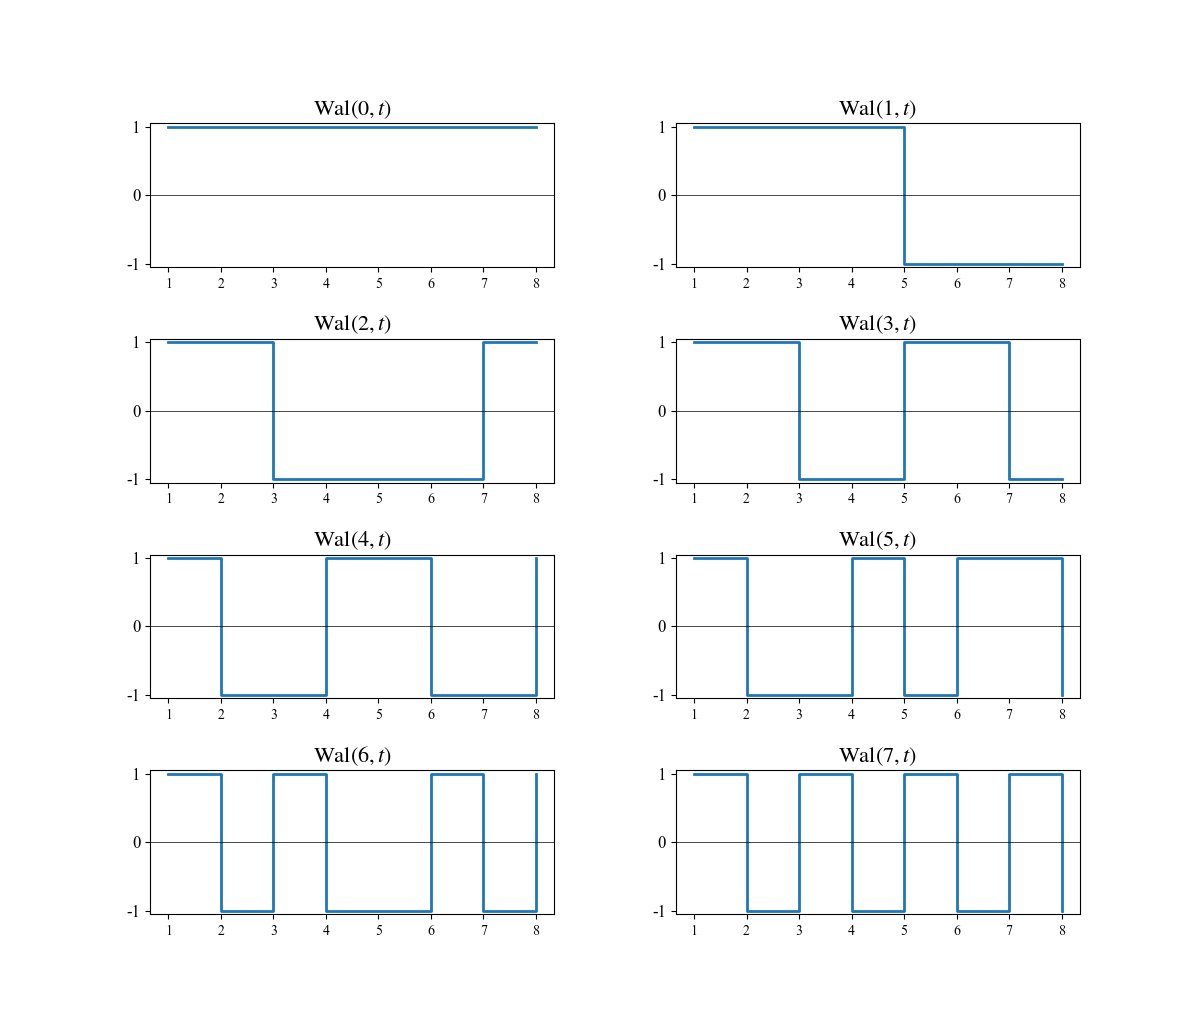
\includegraphics[scale=.5]{Figure_1.png}};
  \end{tikzpicture}
  \]
\end{problem}
\begin{problem}
  For any Hadamard matrix
\[
H_{2^n}=\mqty[H_{2^{n-1}} & H_{2^{n-1}} \\ H_{2^{n-1}} & -H_{2^{n-1}} ].
\]
If we split a $2^n \times 1$ vector into two vectors $x^1_{2^{n-1}}, \ x^2_{2^{n-1}}$ it is easy to show that 
\[
H_{2^n}x = \mqty[H_{2^{n-1}} x^1_{2^{n-1}} + H_{2^{n-1}} x^2_{2^{n-1}} \\ H_{2^{n-1}} x^1_{2^{n-1}} - H_{2^{n-1}} x^2_{2^{n-1}} ].
\]
In turn, for $H_{2^{n-1}} x_1 $ we can repeat the same procedure. We do this until we reach the simple evaluation for $H_2$. As shown 
in the algorithm below, for each of the $n/2$ times we repeat this procedure, we have two recursive calls, so a total of $n$ recursive calls. 
\begin{algorithm}[H]
\caption{Recursive Hadamard Transform}
\begin{algorithmic}[1]
\Require $x \in \mathbb{R}^{2^n}$, integer $n \ge 1$
\Ensure $y = H_{2^n} x$  
\Function{Hadamard}{$x, n$}
\If{$n = 1$}
\State \Return $\begin{bmatrix} x_1 + x_2 & x_1 - x_2 \end{bmatrix}$
\EndIf
\State Split $x$ into $x^{1}, x^{2} \in \mathbb{R}^{2^{n-1}}$
\State $y^{1} \gets \Call{Hadamard}{x^{1}, n-1}$
\State $y^{2} \gets \Call{Hadamard}{x^{2}, n-1}$
\State \Return $\begin{bmatrix}
y^{1} + y^{2} &
y^{1} - y^{2}
\end{bmatrix}$
\EndFunction
\end{algorithmic}
\end{algorithm}
\end{problem}

\section*{Chapter 5}
\stepcounter{section}
\begin{problem}
  Pick two vectors $v \in V$ and $w \in W$; then $v+w \in V \cup W$. There are three cases: first, $v+w \in (V \cup W) \setminus W$ which contradicts the 
  fact that $V$ is a subspace unless $W \subseteq V$. Second, $v+w \in (V \cup W) \setminus V$ which contradicts the fact that $W$ is a subspace unless 
  $V \subseteq W$. Finally $v+w \in V \cap W$ which again contradicts the subspace properties of $V, \ W$ unless $V = W$. 
  We conclude that we either have $V \subseteq W$ or $W \subseteq V$.
\end{problem}
\begin{problem}
  First pick $x$ such that $f(x)=0$. If $x \in \im f$ then $x=f(y)$ for some $y \in E$. From the definition of $f$, $f(x)=f \circ f(y)=f(y)$ so $y \in \ker f$.
  Therefore $f(y)=0$ which means that only if $x=0$ then $x \in \ker f, \ \im f$. Hence $\ker f \cap \im f = \qty{0}$ and $E$ is the direct sum of these two 
  subspaces. 
\end{problem}
\begin{problem}
\subno{1.} From the definition of $\ker a$, $(u_1,\ldots,u_p)\in \ker a$ if 
\[
u_1 + \cdots+ u_i + \cdots + u_p = 0.
\]
This is equivalent to $u_i = -\sum_{j \neq i} u_j$ for all $i=1,\ldots,p$. This can only hold if  
\[
  u_i \in U_i \cap \sum_{j \neq i} U_j, \quad i=1,\ldots,p.
\]
Hence we obtain sets $Z_1,\ldots, Z_p$.

If we require that $U_i \cap \sum_{j \neq i} U_j=\qty{0}$ it does not follow that $Z_i=\qty{0}$. For the other subspaces we could have 
$U_j \cap \sum_{k \neq j} U_k \neq \qty{0}$ and this would produce nonzero elements in $Z_i$. If we require that $U_i \cap \sum_{j \neq i} U_j=\qty{0}$ for all $i=1,\ldots,p$ 
then $Z_i=\qty{0}$ for all $i=1,\ldots,p$ and $\ker a=\qty{0}$.
\subno{2.} If the condition given holds then $\ker a=\qty{0}$ and $a$ is injective. When map $a$ is injective then it is a linear isomorphism between
$U_1 \times \cdots \times U_p$ and $U_1 \oplus \cdots \oplus U_p$. Hence $U_1+\cdots+U_p$ is a direct sum. Conversely, if $U_1+\cdots+U_p$ is a direct sum 
then $a$ is an injective linear map and $\ker a=\qty{0}$. From the definition of $\ker a$ this can hold only if $U_i \cap \sum_{j \neq i} U_j=\qty{0}$ for all $i=1,\ldots,p$.
This completes the proof.
\end{problem}
\begin{problem}
\subno{1.} From the definition, for some vector $x \in E$
\[
\id_E x = x = f_1 x + \cdots + f_p x.
\] 
Therefore $x \in \sum_i \im f_i$ and since $\im \id_E = E$ we must also have $E = \sum_i \im f_i$. If we assume that $f_i \circ f_j=0$ then 
$\im f_i \cap \im f_j = \qty{0}$ if $i \neq j$ and so $E = \im f_1 \oplus \cdots \oplus \im f_p$. Therefore $f_i$ partitions $E$ and so 
it must be a projection with the property $f_i \circ f_i = f_i$. Conversely, note that for any linear map $f$ the trace of 
its matrix representation is basis independent. We have already seen that given a basis transformation any matrix $F$ has the 
property
\[
F' = P F P^{-1}
\]
where $P$ is the change of basis matrix. From the cyclical property of the trace operator 
\[
\tr(F')=\tr(P F P^{-1})=\tr(P^{-1}PF)=\tr(F)
\]
and so the trace of a linear map is invariant. Since 
\[
\id_E = f_1 + \cdots + f_p 
\]
it follows that 
\[
\dim E =\tr(\id_E) = \tr(f_1) + \cdots + \tr(f_p).
\]
Now under some basis the matrix of a projection $f$ has the form $\mqty[I_r & O \\ O & O]$ where $r$ is the dimension of $\im f$.
$\tr f = \rank f$ and so we must have 
\[
\dim E = \rank f_1 + \cdots + \rank f_p.
\]
This only holds if $\im f_i \cap \im f_j = \qty{0}$ for any $i \neq j$. To see this note that  
\[
\dim \id_E = \rank f_1 + \rank (f_2+ \cdots f_p) - \dim (\im f_1 \cap \im( f_2+ \cdots + f_p)).  
\]
If we write the same for $\rank (f_2+ \cdots f_p)$ until it is fully resolved we obtain 
\[
\dim \id_E = \rank f_1 + \cdots + \rank f_p + \underbrace{\hhd}_{\text{lots of intersections}}.
\]
Only if all intersections have $0$ as their common element does equality hold.

Define the projection operator $\pi_i: E \to U_i$. This, obviously, has the property $\pi_i \circ \pi_i = \pi_i$. Next, from the property given 
\begin{align*}
  (\pi_1 + \cdots + \pi_n )\circ (\pi_1 + \cdots + \pi_n ) & = \pi_n \circ \pi _n + \pi_n \circ (\pi_1 +\cdots + \pi_{n-1} ) + (\pi_1 +\cdots + \pi_{n-1} ) \circ \pi_n\\
  & \kern5ex  + (\pi_1 +\cdots + \pi_{n-1} ) \circ (\pi_1 +\cdots + \pi_{n-1} ) \\
& = \pi_n + (\pi_1 +\cdots + \pi_{n-1} ) \circ (\pi_1 +\cdots + \pi_{n-1} ). 
\end{align*}
Repeating the same procedure for all partial sums we obtain 
\begin{align*}
  (\pi_1 + \cdots + \pi_n )\circ (\pi_1 + \cdots + \pi_n ) & = \pi_1 + \cdots + \pi_n
\end{align*}
and so $\pi=\pi_1 + \cdots + \pi_n$ is a projection. 
If we replace $\id_E$ (which is a projection) 
with $\pi$ and $E$ with $U_1+\cdots+U_p$ in the first part of this question we 
obtain the same results. Hence we conclude that $\pi_i \circ \pi_j=0$ for $i \neq j$ and so
$U_1 + \cdots + U_p$ is a direct sum. Conversely, if $U_1 + \cdots + U_p$ is a direct sum then $\pi_i \circ \pi_j=0$ for $i \neq j$
and the property given holds. 
\end{problem}
\begin{problem}
\subno{1.} An involution is invertible since if $f(x)=0$ we also have $f(f(x))=x$. Since $f$ is a linear map $x=0$ 
and so $\ker f=\qty{0}$. Furthermore, $f \circ f = \id \Rightarrow f^{-1} = f$. 
\subno{2.} $f$ has the property  
\[
\begin{aligned}
f\qty(\frac{u+f(u)}{2}) & =\frac{f(u)+f(f(u))}{2}=u, \quad u \in E_1 \\
f\qty(\frac{u+f(u)}{2}) & =\frac{f(u)+f(f(u))}{2}=0, \quad u \in E_{-1} 
\end{aligned}
\] 
and 
\[
\begin{aligned}
f\qty(\frac{u-f(u)}{2}) & =\frac{f(u)-f(f(u))}{2}=0, \quad u \in E_1 \\
f\qty(\frac{u-f(u)}{2}) & =\frac{f(u)-f(f(u))}{2}=-u, \quad u \in E_{-1}   
\end{aligned}
\] 
Therefore $\pi_1 = f \circ \frac12 (f + \id)$ is a projection $E \to E_1$ while $\pi_{-1} = f \circ \frac12 (f - \id)$ is a projection $E \to E_{-1}$ 
($\ker \pi_1 = E_{-1}$ and $\ker \pi_{-1} = E_1$). Since for any $u \in E$
\[
u = \frac{u+f(u)}{2} + \frac{u-f(u)}{2}
\]
we must have  
\[
f(E)= E =\im  \pi_1 +  \im \pi_{-1} 
\]
since for $f$ to be invertible it must be bijective. Combining this with the kernels of $\pi_1, \ \pi_{-1}$ 
we conclude that $E = E_1 \oplus E_{-1}$. 
\subno{3.} Since $f$ is an involution, if $F$ is the matrix representation of $f$ in some basis, then $F^2=I_n$. Write $F$ in block form 
\[
F = \mqty[ A & B \\ C & D].
\]
Since $\pi_1 = f \circ \frac12 (f + \id)$, we have
\[
\mqty[ A & B \\ C & D] \frac12 \qty(\mqty[ A & B \\ C & D] + \mqty[ I_k & O \\ O & I_{n-k}])
=
\frac12 \qty(\mqty[ I_k & O \\ O & I_{n-k}] + \mqty[ A & B \\ C & D])
=
\mqty[I_k & O \\ O & O].
\]
The matrix on the right-hand side is the matrix representation of $\pi_1$ in the same basis. From the above equation we have $A^2 + AB = A$ and $CA + CD = C$. Since $F^2=I_n$ 
it is easy to see that $B=C=O$, $A=I_k$ and $D=I_{n-k}$. We can check that 
\[
\mqty[ I_k & O \\ O & -I_{n-k}] \mqty[ I_k & O \\ O & -I_{n-k}] =\mqty[ I_k & O \\ O & I_{n-k}] 
\]
and 
\[
\frac12 \qty(\mqty[ I_k & O \\ O & I_{n-k}] - \mqty[ I_k & O \\ O & -I_{n-k}])
=
\mqty[O & O \\ O & I_{n-k}].
\]
the matrix for $\pi_{-1}$. It is easier to give a geometric interpretation of the action of $f$ if we consider matrix 
$F$ in $\R^2$. If under some basis $F$ is represented by $\smqty[1 & 0 \\ 0 & -1]$ then $f$ is a reflection across the $x$-axis. 
For vectors like $\vec{x}=\mqty(x & 0)$, $F \vec{x}=\vec{x}$ while for vectors like $\vec{y}=\mqty(0 & y)$, $F \vec{y}=-\vec{y}$.
Any other vector $\mqty(x & y)$ is also reflected across the $x$-axis.
If we extend the same idea to $\R^n$ we can see that $f$ produces the reflection of any vector across the subspace $E_1$.
\end{problem}
\begin{problem}
 An upper Hessenberg matrix looks something like this 
 \[ H=
 \begin{tikzpicture}[baseline={([yshift=-2.5ex]current bounding box.center)}]
  \matrix (m) [matrix of math nodes, row sep=0ex, column sep=0ex, nodes in empty cells, nodes={shape=rectangle,minimum height=3ex, minimum width=3ex,anchor=center},] {
           & \scriptstyle k=1 & \scriptstyle k=2 & \scriptstyle k=3 & \hd & \scriptstyle k=n \\
  \scriptstyle j=1  &    0 & * & * & \hd & * \\
  \scriptstyle j=2  &    0 & 0 & * & \hd & * \\ 
  \scriptstyle j=3  &    0 & 0 & 0 & \hd & * \\
   \vd  &    \vd & \vd & \vd & \rdd & \vd \\
  \scriptstyle j=n  &    0 & 0 & 0 & \hd & 0 \\
  };
  \node[fit= (m-2-2.north west) (m-6-6.south east), left delimiter={[}, right delimiter={]},inner sep=0ex] {};
 \end{tikzpicture},
 \] 
 while an unreduced upper Hessenberg matrix looks like this
 \[ H_u =
  \begin{tikzpicture}[baseline={([yshift=-1.5ex]current bounding box.center)}]
    \matrix (m) [matrix of math nodes, row sep=0ex, column sep=0ex, nodes in empty cells, nodes={shape=rectangle,minimum height=3ex, minimum width=3ex,anchor=center},] {
           & \scriptstyle k=1 & \scriptstyle k=2 & \scriptstyle k=3 & \hd & \scriptstyle k=n-1 & \scriptstyle k=n \\
      \scriptstyle j=1  & 0 & * & * & \hd   & *  & * \\
      \scriptstyle j=2  & * & 0 & * & \hd   & *  & * \\ 
      \scriptstyle j=3  & 0 & * & 0 & \hd   & *  & * \\
       \vd  & \vd & \vd & \vd   & \rdd  & \vd & \vd \\
      \scriptstyle j=n-1  & 0 & 0 & 0 & \hd & 0  & * \\
      \scriptstyle j=n  & 0 & 0 & 0 & \hd   & *  &  0 \\
    };
    \node[fit= (m-2-2.north west) (m-7-7.south east), left delimiter={[}, right delimiter={]},inner sep=0ex] {};
  \end{tikzpicture}.
 \]
 Consider a vector $x$ such that $Hx=0$. We obtain the following system of equations
\[
\begin{aligned} 
0 \cdot x_1 + h_{12}x_2 + h_{13}x_3 + \cdots + h_{1n-2}x_{n-3} + h_{1n-1}x_{n-1} + h_{1n}x_n & = 0 \\
h_{21} \cdot x_1 + 0 \cdot x_2 +h_{23} x_3   + \cdots + h_{2n-2}x_{n-2} + h_{2n-1}x_{n-1} + h_{2n}x_n & = 0 \\
 \vdots \kern30ex & \\        
0 \cdot x_1 + 0 \cdot x_2 + 0 \cdot x_3 + \cdots + h_{n-1,n-2} \cdot x_{n-2} + 0 \cdot x_{n-1} + h_{n-1,n}x_n & = 0 \\
0 \cdot x_1 + 0 \cdot x_2 + 0 \cdot x_3 + \cdots + 0 \cdot x_{n-2} + h_{n,n-1}x_{n-1} + 0 \cdot x_n & = 0
\end{aligned}
\]
From the last equation we have $x_{n-1}=0$. 
From the second to last equation we have 
$$x_{n-2}=-\frac{h_{n-1,n}}{h_{n-1,n-2}}x_n.$$
From the third to last equation we have
$$x_{n-3}=-\frac{h_{n-2,n}}{h_{n-2,n-3}}x_n.
$$
etc. Continuing in this way we can express all $x_i$ as a function of $x_n$. Hence the null space of $H$ is one-dimensional 
and so $\dim(\ker(H))=1$.
\end{problem}
\begin{problem} 
  \subno{1.} If $Ax=0$ then $A^\T Ax =0$. Now suppose that for some vector $y$, $Ay \neq 0$ is in the nullspace of $A^\T$. 
  Then we can write  
  \[
  y^\T A^\T A y =0 \Rightarrow \norm{A y}^2=0.
  \]
  This is only possible if $Ay=0$ which contradicts the assumption. Hence $\ker(A) = \ker(A^\T A)$. Since by the Rank-Nullity Theorem
  \[
   k = \rank(A^\T A) + \dim\ker(A^\T A)  
  \]
  and 
  \[
   k = \rank(A) + \dim\ker( A)  
  \]
  use of $\ker(A^\T A)=\ker(A)$ completes the proof. Exactly the same argument can be used to show that $\rank(A A^\T)=\rank(A)$.
\subno{2.} Since the columns of $A$ are linearly independent vectors the only vector $x$ for which $Ax=0$ is the zero vector.
  Hence $\ker(A)=\qty{0}$ and so $\ker(A^\T A)=\qty{0}$. From the Rank-Nullity Theorem we have $\rank(A^\T A)=k$. It is invertible 
  since it is surjective (its columns span a $k$ dimensional space) and injective.
  For $P$, 
  \[
  P^2 = A(A^\T A)^{-1} A^T A(A^\T A)^{-1} A^\T  =
  A(A^\T A)^{-1} (A^\T A)(A^\T A)^{-1} A^\T= A(A^\T A)^{-1} A^\T = P 
  \]
  and, using $(ABC)^\T=C^\T B^\T A^\T$
  \[
  P^\T = A (A^\T A)^{-\T} A^\T = A (A^\T A)^{-1} A^\T = P.
  \]
  When $k=1$, $A$ is a column vector and 
  \[
  P = \norm{A}^{-2}AA^\T
  \]
  is a rank-1 projection matrix that maps any vector onto the line spanned by $A$.
\subno{3.} We note again that since 
\[
A = \mqty[ a_1 & \cdots & a_k]
\]  
then 
\[
A x = x_1 a_1 + \cdots + x_k a_k.
\]
and so $\im A = \sspan \qty(a_1, \ldots, a_k)$.
Now 
$$
P x = A(A^\T A)^{-1} A^\T x = A((A^\T A)^{-1} A^\T x) 
$$
and so $\im P \subseteq \im A$. Next if $x=Ay$ then 
\[
P Ay = A(A^\T A)^{-1} A^\T A y = Ay 
\] 
and since $P$ is a projection, $\im A \subseteq \im P$. Hence $\im P = \im A$. For the nullspace of $P$ 
it is clear that if $A^\T x =0$ then $P x =0$. The nullspace of $A$ is $\qty{0}$ and so any vector that 
$(A^\T A)^{-1}$ maps to zero will be part of the nullspace of $P$. Since $A^\T A$ is invertible the only vector 
with this property is the zero vector. Hence $\ker P = \ker A^\T$. We note that a vector $x$ with the property 
$A^\T x=0$ is orthogonal to all columns of $A$ and so $\ker A^\T = (\im A)^\perp$. Since $\im P = \im A$, $\ker P = (\im P)^\perp$ 
and so $\R^n = \ker P \oplus \im P$.
\end{problem}  
\begin{problem}
\subno{1.}
\[
\begin{tikzpicture}
  \node at (0,0) {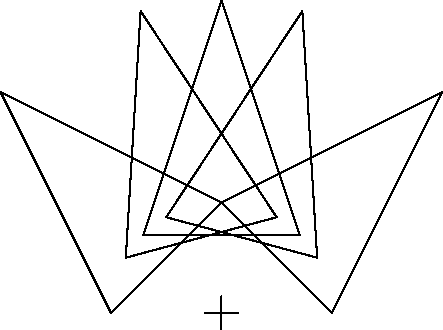
\includegraphics{rotations.pdf}};
\end{tikzpicture}
\]  
\subno{2.}
\[
\qty{
\begin{aligned}
  x\cos\theta  - y \sin\theta  & = x' \\
  x\sin\theta  + y \cos\theta  & = y' \\
\end{aligned}
}
\Leftrightarrow
\qty{ 
\begin{aligned}
  x' \cos\theta + y' \sin\theta & = x \\
  -x' \sin\theta + y' \cos\theta & = y\\
\end{aligned}
}
\]
Therefore 
\[
R_\theta^{-1}=
\mqty[\cos\theta & - \sin\theta \\ \sin\theta & \cos\theta]^{-1}
=
\mqty[\cos\theta & \sin\theta \\ -\sin\theta & \cos\theta]=
\mqty[\cos(-\theta) & - \sin(-\theta) \\ \sin(-\theta) & \cos(-\theta)]=R_{-\theta}.
\]
\subno{3.}
\begin{align*}
  R_\theta R_\phi & =
  \mqty[\cos\theta & - \sin\theta \\ \sin\theta & \cos\theta]
  \mqty[\cos\phi & - \sin\phi \\ \sin\phi & \cos\phi] \\ 
  &= \mqty[
    \cos\theta \cos\phi - \sin\theta \sin\phi & -\cos\theta \sin\phi - \sin\theta \cos\phi \\
    \sin\theta \cos\phi + \cos\theta \sin\phi & -\sin\theta \sin\phi + \cos\theta \cos\phi
  ]  \\
  & = \mqty[
    \cos(\theta+\phi) & -\sin(\theta+\phi) \\
    \sin(\theta+\phi) & \cos(\theta+\phi)
  ] = R_{\theta+\phi} = R_{\phi+\theta} = R_\phi R_\theta.
\end{align*}

Denote the set of plane rotation matrices by $\cR$. This set equipped with the binary operation of matrix multiplication 
is a commutative group if it satisfies the following properties:
\begin{enumerate}[1.]
  \item Commutative law: $R_\theta  R_\phi = R_{\phi}  R_\theta $ as shown above. 
  \item Associative law: 
  $R_\theta (R_\phi  R_\psi) = (R_\theta  R_\phi) R_\psi$ since $\theta+(\phi+\psi)=(\theta+\phi)+\psi$. 
  \item For all $R_\theta \in \cR$, $R_0 R_\theta = R_\theta R_0 = R_\theta$ ($R_0$ is the identity element).
  \item For all $R_\theta \in \cR$, $R_{\theta}R_{-\theta}=R_{-\theta}R_{\theta}=R_0$ (existence of inverse). 
\end{enumerate} 
\end{problem}
\begin{problem}
\subno{1.} $c^\T=\mqty(c_1 & c_2)$ is a unique fixed point if 
\[
c = R_\theta c + a \Leftrightarrow (I-R_\theta) c = a .
\] 
$I-R_\theta$ is invertible since 
\[
\mqty[1 - \cos\theta & -\sin\theta \\ \sin\theta & 1 - \cos\theta] \mqty(x \\ y)=0 \Rightarrow \mqty(x \\ y) = \mqty(0 \\ 0) , 
\quad \theta \in (0,2\pi).
\]
This is easy to prove since the rows of $I-R_\theta$ are orthogonal vectors and, if a third vector $\mqty(x & y)$ is orthogonal 
to these two vectors, the vector space must have dimension 3 which does not hold. To find the inverse make the assumption that 
\[
(I-R_\theta) \lambda R_\phi = I
\]
where $\lambda$ is a scalar. Then we must have 
\[
\lambda (R_\phi - R_{\phi+\theta}) = I.
\]
Since 
\[
R_\psi + R_{-\psi} = 2\cos\psi I
\]
and 
\[
-R_\psi = R_{\pm\pi} R_\psi = R_{\pm\pi+\psi}
\]
we must have 
\[
\phi = -(-\pi+\phi+\theta) \Rightarrow \phi = \frac12 (\pi-\theta)
\]
and $\lambda=1/(2\cos\qty(\frac12(\pi-\theta)))=1/(2\sin\qty(\frac12\theta))$.
\subno{2.} It is clear that if 
\[
y=R_\theta x + a
\]
then 
\[
y-c=R_\theta x + a-c.
\]
Next
\[
a - c = (I-R_\theta)c - I c=-R_\theta c.
\]
Hence 
\[
y - c = R_\theta (x - c).
\]
\subno{3.}
\[
\begin{tikzpicture}
  \node at (0,0) {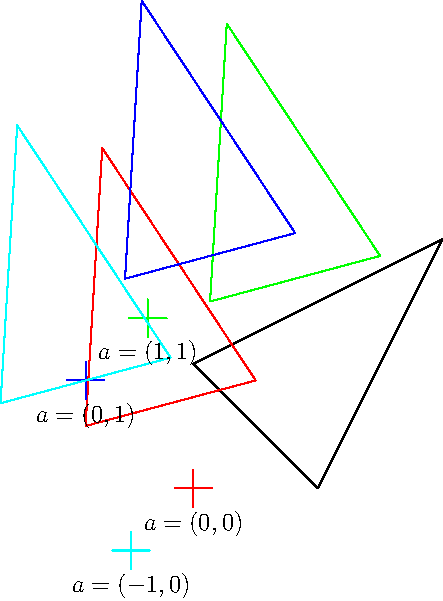
\includegraphics{affine.pdf}};
\end{tikzpicture}
\]  
If $\theta=2k\pi$ then $y=x+a$ so we have a translation. 
\subno{4.}
$R_{\theta,(a_1,a_2)}$ corresponds to the following transformations 
\[
 x \xrightarrow{T} x-c, \; x-c \xrightarrow{R_\theta} y-c , \; y-c \xrightarrow{T} y
\]
where T (resp. R) indicates a translation (resp. rotation). Given $c$ the reverse 
procedure is 
\[
y \xrightarrow{T} y-c, \; y-c \xrightarrow{R_{-\theta}} x-c , \; x-c \xrightarrow{T} x. 
\]
This suggests that the inverse is of the form $R_{-\theta,(a_1,a_2)}$ since both transformations 
use $c$. However given that in the reverse procedure the rotation is by $-\theta$, $(a_1,a_2)$
cannot produce the same $c$. So instead the inverse must be of the form $R_{-\theta,(b_1,b_2)}$.
Since both must produce the same $c$,
\[
\frac{1}{2\sin\frac{\theta}{2}} R_{\frac{\pi}{2}-\frac{\theta}{2}} a
=
-\frac{1}{2\sin\frac{\theta}{2}} R_{\frac{\pi}{2}+\frac{\theta}{2}} b , 
\]
or 
\[
R_{\frac{\pi}{2}-\frac{\theta}{2}} a=-R_{\frac{\pi}{2}+\frac{\theta}{2}} b.
\]
Use $R_{-\pi}=-1$ to get 
\[
R_{\frac{\pi}{2}-\frac{\theta}{2}} a=R_{-\frac{\pi}{2}+\frac{\theta}{2}} b.
\]
Therefore 
\[
b = R_{\frac{\pi}{2}-\frac{\theta}{2}}^2 a =R_{\pi-\theta} a.
\]
\subno{5.}
\[
R_{\alpha,a}x= R_\alpha x + a 
\]
and 
\[
R_{\beta,b}x= R_\beta x + b .
\]
Therefore 
\[
R_{\beta,b} \circ R_{\alpha,a} x = R_\beta R_\alpha x + R_\beta a + b
\]
and so 
\[
R_{\beta,b} \circ R_{\alpha,a} = R_{\alpha+\beta,t}
\]
where $t=R_\beta a + b$.

In general 
\[
R_{\beta,b} \circ R_\alpha x = R_{\alpha+\beta}x + b 
\]
while 
\[
R_\alpha  \circ R_{\beta,b} x = R_{\alpha+\beta}x + R_\alpha b
\]
so the two compositions are different. 

A nonabelian group is a set equiped with a binary operation for 
which 
\begin{enumerate}[1.]
  \item The associative law holds. Use (5) to write 
  \[  
  R_{\alpha,a} \circ (R_{\beta,b} \circ R_{\gamma,c}) =
  R_{\alpha,a} \circ R_{\beta+\gamma,R_\beta c + b} = R_{\alpha+\beta+\gamma,R_{\alpha}(R_\beta c + b)+a}
  \]
  Also 
  \[  
  (R_{\alpha,a} \circ R_{\beta,b}) \circ R_{\gamma,c} =
  R_{\alpha+\beta,R_\alpha b+ a} \circ R_{\gamma,c} = R_{\alpha+\beta+\gamma,R_{\alpha+\beta}c+R_\alpha b+ a}.
  \]
  It is easy to check that the two expressions are equal.
  \item The identity element is $R_{0,0}$ which is an affine map. 
  \item In (4) we have shown the existence of an inverse for every affine map.
\end{enumerate}

To prove that $R_{\beta,b} \circ R_{\alpha,a}$ is not a translation
\[
R_{\beta,b} \circ R_{\alpha,a} = R_{\alpha+\beta,R_\beta a + b}.
\]
This is a translation only if $\alpha+\beta=2\pi k$ for all $k \in \Z$. If $a=0$ its center of rotation is 
\[
c = \frac{1}{2\sin \frac{\alpha+\beta}{2}} R_{\frac{\pi}{2}-\frac{\alpha+\beta}{2}} b.
\]
If $\alpha+\beta=2\pi k$ the translation vector is $R_\beta a + b$.
\end{problem}
\begin{problem}
\subno{1.} $0 \in U$ (since it is a subspace) and so $a \in \cal A$. Affine subspaces of dimension 0 are also called 
vectors. In $\R^2$, an affine subspace of dimension 1 is obtained by the parallel translation of a line by vector $a$ (the same is true 
for $\R^n$). In $\R^3$, an affine subspace of dimension 2 is obtained by the parallel translation of a plane with vector $a$. 

An affine combination of vectors $a+u_i \in \cal A$ is given by 
\[
\sum_i \lambda_i (a+u_i) = a + \sum_i \lambda_i u_i
\]
since $\sum_i \lambda_i =1$
and since $U$ is a subspace, $a+ \sum_i \lambda_i u_i \in \cal A$.
\subno{2.} If $b \in \cal A$ then $b=a+u'$ for some $u' \in U$. Since 
\[ 
a + u = a + u' + u - u' = b + u-u'
\]
and $u-u' \in U$ the desired result follows.
\subno{3.} Since $a \in \cal A$, the zero vector is a member of $U_a$ which is an important requirement for 
$U_a$ to be a subspace. Next note that 
\[
x - a +  y - a = (x + y - a) - a, \qquad x,y,a \in \cal A.
\]
$x+y-a$ is an affine combination and so it is a member of $\cal A$. From the definition of $U_a$,  
$x - a +  y - a \in U_a$ and so this is closed under vector addition. Regarding scalar multiplication 
\[
\lambda (x-a) = (\lambda x - \lambda a + a) - a.
\]
$\lambda x - \lambda a + a$ is another affine combination of members of $\cal A$ and so it is also a member. 
Therefore $\lambda (x-a) \in \cal A$. Finally use the property $x \in {\cal A} \Leftrightarrow x-a \in U_a$
to conclude that ${\cal A}=a + U_a$.

If $a,b \in \cal A$ then assume that it is possible to have $u \in U_a$ with $u \not\in U_b$. Since 
$u=x-a=x+b-a-b$ and $x,a,b \in \cal A$, $x+b-a$ is an affine combination and so it is also a member of 
$\cal A$. Hence $x-a \in U_b$ and we have a contradiction. So $U_a=U_b$; it is also true that $U_a=U$ since 
if $u \in U_a, \ x, \ z \in \cal A$ 
\[
u = z - a = z - a + x - x = y - x
\]
with $y \in \cal A$ since $z-a+x$ is an affine combination. 
\subno{4.} If two affine subspaces $\cal A,\, \cal B$ have the same direction then 
${\cal A}=a + U$ and ${\cal B}= b + U$ for some $a \in \cal A$ and $b \in \cal B$.  
If ${\cal A} \neq {\cal B}$, then assume that, for some $u,u' \in U$, $a+u=b+u'$. For any element 
$v + a \in \cal A$ we can also write it as $v + u' - u + b$. Since $v,u,u' \in U$, $v+u'-u \in U$ and so 
$v + a \in \cal B$. Therefore ${\cal A}={\cal B}$ and we have reached a contradiction. We conclude that 
${\cal A} \cap {\cal B} = \varnothing$ if ${\cal A} \neq {\cal B}$ and they are parallel.
\end{problem}
\begin{problem}
\subno{1.} The $m+1$ vectors are linearly independent if and only if
\[
\lambda_0 \hat{u}_0 + \lambda_1 \hat{u}_1 + \cdots + \lambda_m \hat{u}_m = 0 \Rightarrow \lambda_0=\lambda_1=\cdots=\lambda_m=0.
\]    
Write each vector $\hat{u}_i$ as $(u_1,1)$; the equation above is now  
\[
\lambda_0 ({u}_0,1) + \lambda_1 ({u}_1,1) + \cdots + \lambda_m ({u}_m,1) = (0,0).
\]
From the $n+1$ component we must have
\[
\lambda_0 + \lambda_1 + \cdots + \lambda_m = 0 \Rightarrow \lambda_0 = -\lambda_1 - \cdots - \lambda_m.
\]
Then we can rewrite the original condition as 
\[
\lambda_1 ({u}_1-u_{0},0) + \cdots + \lambda_m ({u}_m-u_0,0) = (0,0).
\]
If $u_1-u_0,\ldots,u_m-u_0$ are independent then the first $n$ components are zero only if 
$\lambda_1=\cdots=\lambda_m=0$. So we obtain the required result.
\subno{2.} This is a simple reworking using (1). Instead of going from 
\[
\lambda_0 + \lambda_1 + \cdots + \lambda_m = 0
\]
to
\[
\lambda_0 = -\lambda_1 - \cdots - \lambda_m
\]
go from 
\[
\lambda_0 + \cdots + \lambda_i + \cdots + \lambda_m = 0
\]
to 
\[
\lambda_i = - \lambda_0 - \cdots - \lambda_{i-1} - \lambda_{i+1} - \cdots - \lambda_m.
\]
\subno{3.} From the $n+1$ affinely independent vectors we obtain $n$ independent vectors 
$u_1-u_0,\ldots,u_n-u_0$ which form a basis of $\R^n$. Therefore for any $v \in \R^n$
\[
v = v_1 (u_1-u_0)+ \cdots + v_n (u_n-u_0), \quad v_1,\ldots,v_n \in \R.
\]
Since $u_0 \in \R^n$ we can write 
\[
v + u_0 = (1-v_1 - \cdots - v_n) u_0 + v_1 u_1 + \cdots + u_n. 
\]
Therefore $v'=v+u_0$ is a linear combination of $u_0,u_1,\ldots,u_n$ with the sum of the 
coefficients equal to one. Since for any $i$, $\qty{u_j-u_i}_{j \neq i}$ also forms a basis of $\R^n$
we obtain the barycentric expansion of any vector. To prove that for any $v \in \R^n$ 
\[
v = u_0 + \lambda_1 e_1 + \cdots + \lambda_n e_n
\]
start with  
\[
v = \lambda_0 u_0 + \lambda_1 u_1 + \cdots + \lambda_n u_n
\]
and use $\lambda_0+\lambda_1+\cdots+\lambda_n=1$, $e_i=u_i-u_0$ to complete the proof. To prove the converse is 
a straightforward conversion of 
\[
v = u_0 + x_1 e_1 + \cdots + x_n e_n
\]
to 
\[
v =(1-(x_1+\cdots+x_n)) u_0 + x_1 u_1 + \cdots + x_n u_n
\]
using $e_i=u_i-u_0$.
\subno{4.} To specify any linear map from $\R^n \to \R^m$ we must specify how each of the
$n$ basis vectors of $\R^n$ maps to a vector in $\R^m$. Since $u_0,\ldots,u_n$ is an affine 
frame of $\R^n$, $u_1-u_0,\ldots,u_n-u_0$ is a basis of $\R^n$. For a linear 
map $\vec{f}$, a set of equations 
\[
\vec{f}(u_i-u_0) = w_i \in \R^m, \quad i=1,\ldots,n
\]
provides a unique specification (Proposition 2.14). Since $\vec{f}$ is a linear map we can rewrite the last equation as 
\[
\vec{f}(u_i)-\vec{f}(u_0)=w_i.
\]
If we define $w_i = v_i - v_0$ then 
\[
\vec{f}(u_i)-\vec{f}(u_0)=v_i-v_0.
\]
Adding  $\vec{f}(u_0)-v_0=b$ we obtain a unique definition for vector $b$. Then the affine 
map $f(u)=\vec{f}(u)+b$ satisfies all the conditions given.
\subno{5.} Any affine map $f$ can be written as $f(u)=\vec{f}(u)+c$ where $\vec{f}$ is a linear map and $c$ is a vector.
Since $a_0,\ldots,a_n$ is an affine frame, $a_1-a_0,\ldots,a_n-a_0$ are basis vectors of $\R^n$. Therefore we can 
produce the standard matrix for $\vec{f}$ as follows 
\[
F=
  \begin{tikzpicture}[baseline={([yshift=-3.ex]current bounding box.center)}]
    \matrix (m) [matrix of math nodes, row sep=0ex, column sep=0ex, nodes in empty cells, nodes={shape=rectangle,minimum height=3ex, minimum width=3ex,anchor=center},] {
        \scriptstyle\vec{f}(a_1-a_0) & \scriptstyle\vec{f}(a_2-a_0) & \hd     & \scriptstyle\vec{f}(a_n-a_0) \\[2ex]
        r_1              &        r_2       & \hd     &     r_n          \\
    };
    \node[fit= (m-2-1.north west) (m-2-4.south east), left delimiter={[}, right delimiter={]},inner sep=2ex] {};
  \end{tikzpicture}  
\]
($r_1,\ldots,r_n \in \R^n$ with $r_i=\vec{f}(a_i-a_0)$; $F$ is a $n \times n$ matrix)

If a translation was another linear map then we could produce a matrix representation for it and combine the two. 
However, a translation is not a linear map (for example, it does not preserve the zero vector). We must find another 
way to represent a translation so that we can derive a matrix for an affine map. 

Any vector $v \in \R^n$ has a barycentric expansion
\[
v = v_1 (a_0-a_n) + \cdots + v_n (a_{n-1}-a_n) + a_n,\quad \sum_{i=1}^n v_i=1.
\]
where $a_0,a_1,\ldots,a_{n-1},a_n \in \R^n$ and $a_0-a_n,a_1-a_n,\ldots,a_{n-1}-a_n$ are a basis of $\R^n$.
Lets pretend that $v$ is really a $\R^{n+1}$ vector with the $n+1$ component always equal to 1. The `basis'
for this representation is $a_0-a_n,\ldots,a_{n-1}-a_n,a_n$. If we want to map $v$ to $v+c$ then, since $v+c$ also 
has a unit $n+1$ component, the transformation matrix has the following form: 
\[
  \begin{tikzpicture}[baseline={([yshift=-5.ex]current bounding box.center)}]
    \matrix (m) [matrix of math nodes, row sep=2ex, column sep=2ex, nodes in empty cells, nodes={shape=rectangle,minimum height=5ex, minimum width=7ex,anchor=center},] {
                \\[2ex]
        v_1+c_1       \\
        v_2+c_2       \\
        \vd      \\
        v_n+c_n       \\
        1     \\
    };
    \node[fit= (m-2-1.north west) (m-6-1.south east), left delimiter={(}, right delimiter={)},inner sep=0ex] {};
  \end{tikzpicture}  
=
  \begin{tikzpicture}[baseline={([yshift=-1.5ex]current bounding box.center)}]
    \matrix (m) [matrix of math nodes, row sep=2ex, column sep=2ex, nodes in empty cells, nodes={shape=rectangle,minimum height=5ex, minimum width=3ex,anchor=center},] {
             &    &   &     &   & \scriptstyle\text{$c$ vector}           \\[2ex]
        1    & 0  & 0 & \hd & 0 & c_1        \\
        0    & 1  & 0 & \hd & 0 & c_2        \\
        \vd  & \vd&\vd&\rdd &\vd & \vd        \\
        0    & 0  & 0 & \hd & 1 & c_n        \\
        0    & 0  & 0 & \hd & 0 & 1        \\
    };
    \node[fit= (m-2-1.north west) (m-6-6.south east), left delimiter={[}, right delimiter={]},inner sep=1.5ex] {};
    \node[fit= (m-2-1.north west) (m-5-5.south east), left delimiter={[}, right delimiter={]},inner sep=0ex] {};
    \node[fit= (m-2-6.north west) (m-6-6.south east), left delimiter={[}, right delimiter={]},inner sep=0ex] {};
    \node[fit= (m-6-1.north west) (m-6-5.south east), left delimiter={[}, right delimiter={]},inner sep=0ex] {};
    \node[fit= (m-2-1.north west) (m-2-5.north east), above delimiter={\{},inner sep=1ex] (im) {};
    \node[fit= (m-6-1.south west) (m-6-5.south east), below delimiter={\}},inner sep=1ex] (zil) {};
    \node at ($(im)+(0,6.5ex)$) {\fontsize{7pt}{8pt}\selectfont $n \times n$ identity matrix};
    \node at ($(zil)-(0,6.5ex)$) {\fontsize{7pt}{8pt}\selectfont $1 \times n$ zero vector};
    \draw[-{Stealth[]}] ($(m-1-6.south)+(0,1ex)$)--(m-2-6.north);
  \end{tikzpicture}  
  \begin{tikzpicture}[baseline={([yshift=-5.ex]current bounding box.center)}]
    \matrix (m) [matrix of math nodes, row sep=2ex, column sep=2ex, nodes in empty cells, nodes={shape=rectangle,minimum height=5ex, minimum width=5ex,anchor=center},] {
                \\[2ex]
        v_1       \\
        v_2       \\
        \vd      \\
        v_n       \\
        1     \\
    };
    \node[fit= (m-2-1.north west) (m-6-1.south east), left delimiter={(}, right delimiter={)},inner sep=0ex] {};
  \end{tikzpicture}  
\]
This form is consistent with the fact that a pure translation is an affine map 
\[
t(u)= \id(u)+ c .
\]
$\id$ is a linear map whose matrix representation is the identity matrix.
For 
\[
f(u) = \vec{f}(u) + c
\]
if we replace the $n \times n$ identity matrix with $F$, the matrix representation for $\vec{f}$, we obtain the matrix for 
the affine map which has the same form as shown in the problem.

If $\hat{a}_i$ is the column vector with the components of $a$ using $a_1-a_0,a_2-a_0,\ldots,a_n-a_0,a_0$ as a basis 
then its affine transformation is given by 
\[
      A \hat{a}_i = \hat{b}_i. 
\]  
If we form a $(n+1)\times(n+1)$ matrix 
\[
\mqty[\hat{a}_0 & \hat{a}_1 & \cdots & \hat{a}_n]
\]
then 
\[
A\mqty[\hat{a}_0 & \hat{a}_1 & \cdots & \hat{a}_n]
=\mqty[A\hat{a}_0 & A\hat{a}_1 & \cdots & A\hat{a}_n]
=\mqty[\hat{b}_0 & \hat{b}_1 & \cdots & \hat{b}_n]
\]
and 
\[
A = \mqty[\hat{b}_0 & \hat{b}_1 & \cdots & \hat{b}_n] 
\mqty[\hat{a}_0 & \hat{a}_1 & \cdots & \hat{a}_n]^{-1}.
\]

Vector $a_0,\ldots,a_n \in \R^n$ can be all converted to $\R^{n+1}$ in the affine frame by augmenting them 
with the compulsory unit $n+1$-component. Hence 
\[
\mqty[\hat{a}_0 & \hat{a}_1 & \cdots & \hat{a}_n] 
=
\mqty[
  \mqty[e_0 \\ 1] & \mqty[e_1 \\ 1] & \cdots & \mqty[e_n \\ 1] & \mqty[0 \\ 1] 
]
\]
which is the matrix shown in the problem. Note that the affine basis 
$$a_0-a_n,a_1-a_n,\ldots,a_{n-1}-a_n,a_n$$ 
corresponds to the first $n$ rows of the matrix. The inverse matrix follows from writing the matrix
in block form:
\[
\mqty[\hat{a}_0 & \hat{a}_1 & \cdots & \hat{a}_n]  = \mqty[\vb*{I}_n & \vb{0} \\ \vb{1}^\T & 1]
\]
where we have used bold letters for vectors and matrices. Lets guess that 
\[
\mqty[\vb*{I}_n & \vb{0} \\ \vb{1}^\T & 1]\mqty[\vb*{I}_n & \vb{0} \\ \vb{1}^\T & 1]^{-1}
=
\mqty[\vb*{I}_n & \vb{0} \\ \vb{1}^\T & 1]\mqty[\vb*{I}_n & \vb{0} \\ \vb*{x}^\T & 1]
=
\mqty[\vb*{I}_n & \vb{0} \\ \vb{1}^\T+\vb*{x}^\T & 1].
\]
Since the last matrix should be the identity matrix set $\vb*{x}=-\vb{1}$ to complete the proof. 
\subno{6.} For any affine combination in $f({\cal A})$ 
\begin{align*}
\sum_i \lambda_i f(a_i) & = \sum_i \lambda_i (\vec{f}(a_i) + c) =\vec{f}\qty(\sum_i\lambda_i a_i) + c \\
& = f\qty(\sum_i \lambda_i a_i) \in f({\cal A})    
\end{align*}
hence $f({\cal A})$ is closed under affine combinations and so is an affine subspace of $\R^n$.

Consider $n$ points $b_1,\ldots,b_n \in \cal B$. These map to 
\[
f^{-1}(b_1),\ldots,f^{-1}(b_n) \in \cal B
\]
vectors in $\R^n$. Take an affine combination of these points 
\[
\lambda_1 f^{-1}(b_1)+\cdots+\lambda_n f^{-1}(b_n).
\]
Since $f$ is an affine map 
\[
f\qty(\lambda_1 f^{-1}(b_1)+\cdots+\lambda_n f^{-1}(b_n))=
\lambda_1f(f^{-1}(b_1))+\cdots+\lambda_n f(f^{-1}(b_n))=\lambda_1 b_1 + \cdots + \lambda_n b_n \in \cal B
\]
and so 
\[
\lambda_1 f^{-1}(b_1)+\cdots+\lambda_n f^{-1}(b_n) \in f^{-1}({\cal B}).
\]
Hence $f^{-1}({\cal B})$ is an affine subspace of $\R^n$.

\end{problem}
\bibliographystyle{plainnat} 
\bibliography{LinOptRefs} 
\end{document}